%!TEX TS-program = xelatex 
%!TEX encoding = UTF-8 Unicode
%
%  my_title
%
%  Created by David Perez on march 2010.
%  Copyright (c) David Perez 2010. All rights reserved.
%

% -*- Mode:TeX -*-



%% The documentclass options along with the pagestyle can be used to generate
%% a technical report, a draft copy, or a regular thesis.  You may need to
%% re-specify the pagestyle after you \include  cover.tex.  For more
%% information, see the first few lines of mitthesis.cls. 

%\documentclass[12pt,vi,twoside]{mitthesis}
%%
%%  If you want your thesis copyright to you instead of MIT, use the
%%  ``vi'' option, as above.
%%
%\documentclass[12pt,twoside,leftblank]{mitthesis}
%%
%% If you want blank pages before new chapters to be labelled ``This
%% Page Intentionally Left Blank'', use the ``leftblank'' option, as
%% above. 

%For the final thesis
\documentclass[12pt,vi]{mitthesis}
\pagestyle{plain} 
 
%for technical report
%\documentclass[12pt,vi,twoside]{mitthesis}
%\pagestyle{plain}

%for draft
%\documentclass[11pt,singlespace,draft]{mitthesis}
%\pagestyle{drafthead}


%%package for TODO lists, comments, annotations on pdf, with colors
\usepackage[disable, spanish, colorinlistoftodos]{todonotes}
%%el comando de abajo hace el trabajo automaticamente identificando si es un
%%draft
%\usepackage[obeyDraft]{todonotes}
%%los posibles COLORES usados para \todo[color=green!40]{test12} son:
%%green, red, blue!20!white (para mezclar dos colores)
%%la UBICACION del comentario, en el borde o entre parrafos:
%%\todo[noline]{A note with no line ...} noline o line o inline
%%\missingfigure[figwidth=6cm]{Testing a long text string}


\usepackage{lgrind}

%% in case I include .eps versions of all figures for those w/o pdftex
\usepackage{ifpdf}
\ifpdf
\usepackage[pdftex]{graphicx}
\else
\usepackage{graphicx}
\fi

\usepackage{amsmath,amssymb,amsfonts} % easily align arrays of equations
\usepackage{hyperref} % hyperlinks
\usepackage{subfig} % multi-part figures
\usepackage{pdfpages} % makes it easy to insert all those nsigmapi fits


% Feynman diagrams
\usepackage{feynmp}
\DeclareGraphicsRule{*}{mps}{*}{}


%%%%%%%%%%%%%%%%%%%%begin code formatting%%%%%%%%%%%%%%%%%%%%%%%%%%%%%%%%%
%paquete para agregar codigo fuente
%\usepackage{listings}
\usepackage{listings}
\usepackage{courier}
\lstset{
         basicstyle=\footnotesize\ttfamily, % Standardschrift
         %numbers=left,               % Ort der Zeilennummern
         numberstyle=\tiny,          % Stil der Zeilennummern
         %stepnumber=2,               % Abstand zwischen den Zeilennummern
         numbersep=5pt,              % Abstand der Nummern zum Text
         tabsize=2,                  % Groesse von Tabs
         extendedchars=true,         %
         breaklines=true,            % Zeilen werden Umgebrochen
         keywordstyle=\color{red},
                frame=b,         
 %        keywordstyle=[1]\textbf,    % Stil der Keywords
 %        keywordstyle=[2]\textbf,    %
 %        keywordstyle=[3]\textbf,    %
 %        keywordstyle=[4]\textbf,   \sqrt{\sqrt{}} %
         stringstyle=\color{white}\ttfamily, % Farbe der String
         showspaces=false,           % Leerzeichen anzeigen ?
         showtabs=false,             % Tabs anzeigen ?
         xleftmargin=17pt,
         framexleftmargin=17pt,
         framexrightmargin=5pt,
         framexbottommargin=4pt,
         %backgroundcolor=\color{lightgray},
         showstringspaces=false      % Leerzeichen in Strings anzeigen ?        
 }
 \lstloadlanguages{% Check Dokumentation for further languages ...
         %[Visual]Basic
         %Pascal
         %C
         %C++
         %XML
         %HTML
         Java
}
    %\DeclareCaptionFont{blue}{\color{blue}} 

  %\captionsetup[lstlisting]{singlelinecheck=false, labelfont={blue}, textfont={blue}}
\usepackage{caption}
\DeclareCaptionFont{white}{\color{white}}
\DeclareCaptionFormat{listing}{\colorbox[cmyk]{0.43, 0.35, 0.35,0.01}{\parbox{\textwidth}{\hspace{15pt}#1#2#3}}}
\captionsetup[lstlisting]{format=listing,labelfont=white,textfont=white, singlelinecheck=false, margin=0pt, font={bf,footnotesize}}

%%%%%%%%%%%%%%%%%%%%end code formatting%%%%%%%%%%%%%%%%%%%%%%%%%%%%%%%%%%%%%%%%


\begin{document}

% -*-latex-*-
% $Log: cover.tex,v $
% Revision 1.8  2008/05/13 15:02:15  jdreed
% Degree month is June, not May.  Added note about prevdegrees.
% Arthur Smith's title updated
%
% Revision 1.7  2001/02/08 18:53:16  boojum
% changed some \newpages to \cleardoublepages
%
% Revision 1.6  1999/10/21 14:49:31  boojum
% changed comment referring to documentstyle
%
% Revision 1.5  1999/10/21 14:39:04  boojum
% *** empty log message ***
%
% Revision 1.4  1997/04/18  17:54:10  othomas
% added page numbers on abstract and cover, and made 1 abstract
% page the default rather than 2.  (anne hunter tells me this
% is the new institute standard.)
%
% Revision 1.4  1997/04/18  17:54:10  othomas
% added page numbers on abstract and cover, and made 1 abstract
% page the default rather than 2.  (anne hunter tells me this
% is the new institute standard.)
%
% Revision 1.3  93/05/17  17:06:29  starflt
% Added acknowledgements section (suggested by tompalka)
% 
% Revision 1.2  92/04/22  13:13:13  epeisach
% Fixes for 1991 course 6 requirements
% Phrase "and to grant others the right to do so" has been added to 
% permission clause
% Second copy of abstract is not counted as separate pages so numbering works
% out
% 
% Revision 1.1  92/04/22  13:08:20  epeisach

% NOTE:
% These templates make an effort to conform to the MIT Thesis specifications,
% however the specifications can change.  We recommend that you verify the
% layout of your title page with your thesis advisor and/or the MIT 
% Libraries before printing your final copy.
\title{An Optimizing Compiler for Low-Level Floating Point Operations}

\author{Lucien William Van Elsen}
% If you wish to list your previous degrees on the cover page, use the 
% previous degrees command:
%       \prevdegrees{A.A., Harvard University (1985)}
% You can use the \\ command to list multiple previous degrees
%       \prevdegrees{B.S., University of California (1978) \\
%                    S.M., Massachusetts Institute of Technology (1981)}
\department{Department of Electrical Engineering and Computer Science}

% If the thesis is for two degrees simultaneously, list them both
% separated by \and like this:
% \degree{Doctor of Philosophy \and Master of Science}
\degree{Bachelor of Science in Computer Science and Engineering}

% As of the 2007-08 academic year, valid degree months are September, 
% February, or June.  The default is June.
\degreemonth{June}
\degreeyear{1990}
\thesisdate{May 18, 1990}

%% By default, the thesis will be copyrighted to MIT.  If you need to copyright
%% the thesis to yourself, just specify the `vi' documentclass option.  If for
%% some reason you want to exactly specify the copyright notice text, you can
%% use the \copyrightnoticetext command.  
%\copyrightnoticetext{\copyright IBM, 1990.  Do not open till Xmas.}

% If there is more than one supervisor, use the \supervisor command
% once for each.
\supervisor{William J. Dally}{Associate Professor}

% This is the department committee chairman, not the thesis committee
% chairman.  You should replace this with your Department's Committee
% Chairman.
\chairman{Arthur C. Smith}{Chairman, Department Committee on Graduate Theses}

% Make the titlepage based on the above information.  If you need
% something special and can't use the standard form, you can specify
% the exact text of the titlepage yourself.  Put it in a titlepage
% environment and leave blank lines where you want vertical space.
% The spaces will be adjusted to fill the entire page.  The dotted
% lines for the signatures are made with the \signature command.
\maketitle

% The abstractpage environment sets up everything on the page except
% the text itself.  The title and other header material are put at the
% top of the page, and the supervisors are listed at the bottom.  A
% new page is begun both before and after.  Of course, an abstract may
% be more than one page itself.  If you need more control over the
% format of the page, you can use the abstract environment, which puts
% the word "Abstract" at the beginning and single spaces its text.

%% You can either \input (*not* \include) your abstract file, or you can put
%% the text of the abstract directly between the \begin{abstractpage} and
%% \end{abstractpage} commands.

% First copy: start a new page, and save the page number.
\cleardoublepage
% Uncomment the next line if you do NOT want a page number on your
% abstract and acknowledgments pages.
% \pagestyle{empty}
\setcounter{savepage}{\thepage}
\begin{abstractpage}
% $Log: abstract.tex,v $
% Revision 1.1  93/05/14  14:56:25  starflt
% Initial revision
% 
% Revision 1.1  90/05/04  10:41:01  lwvanels
% Initial revision
% 
%
%% The text of your abstract and nothing else (other than comments) goes here.
%% It will be single-spaced and the rest of the text that is supposed to go on
%% the abstract page will be generated by the abstractpage environment.  This
%% file should be \input (not \include 'd) from cover.tex.
In this thesis, I designed and implemented a compiler which performs
optimizations that reduce the number of low-level floating point operations
necessary for a specific task; this involves the optimization of chains of
floating point operations as well as the implementation of a ``fixed'' point
data type that allows some floating point operations to simulated with integer
arithmetic.  The source language of the compiler is a subset of C, and the
destination language is assembly language for a micro-floating point CPU.  An
instruction-level simulator of the CPU was written to allow testing of the
code.  A series of test pieces of codes was compiled, both with and without
optimization, to determine how effective these optimizations were.

\end{abstractpage}

% Additional copy: start a new page, and reset the page number.  This way,
% the second copy of the abstract is not counted as separate pages.
% Uncomment the next 6 lines if you need two copies of the abstract
% page.
% \setcounter{page}{\thesavepage}
% \begin{abstractpage}
% % $Log: abstract.tex,v $
% Revision 1.1  93/05/14  14:56:25  starflt
% Initial revision
% 
% Revision 1.1  90/05/04  10:41:01  lwvanels
% Initial revision
% 
%
%% The text of your abstract and nothing else (other than comments) goes here.
%% It will be single-spaced and the rest of the text that is supposed to go on
%% the abstract page will be generated by the abstractpage environment.  This
%% file should be \input (not \include 'd) from cover.tex.
In this thesis, I designed and implemented a compiler which performs
optimizations that reduce the number of low-level floating point operations
necessary for a specific task; this involves the optimization of chains of
floating point operations as well as the implementation of a ``fixed'' point
data type that allows some floating point operations to simulated with integer
arithmetic.  The source language of the compiler is a subset of C, and the
destination language is assembly language for a micro-floating point CPU.  An
instruction-level simulator of the CPU was written to allow testing of the
code.  A series of test pieces of codes was compiled, both with and without
optimization, to determine how effective these optimizations were.

% \end{abstractpage}

\cleardoublepage

\section*{Acknowledgments}

This is the acknowledgements section.  You should replace this with your
own acknowledgements.

%%%%%%%%%%%%%%%%%%%%%%%%%%%%%%%%%%%%%%%%%%%%%%%%%%%%%%%%%%%%%%%%%%%%%%
% -*-latex-*-


\pagestyle{plain}
  % -*- Mode:TeX -*-
%% This file simply contains the commands that actually generate the table of
%% contents and lists of figures and tables.  You can omit any or all of
%% these files by simply taking out the appropriate command.  For more
%% information on these files, see appendix C.3.3 of the LaTeX manual. 


\tableofcontents
\newpage
\printglossaries
%\printglossary[title={Acronyms}]
\newpage
\listoffigures
\newpage
\listoftables


\begin{fmffile}{feynman-diagrams}




%\\.
%\\. 
%\\.
%\\.
%\todo[inline]{Agregar la secci\'on del cover}
%	Debo agregar una hoja donde indique que estos cap\'itulos son
%	el marco teorico de la investigaci\'on, dicho comando para
%	agregar la palabra parte A por ejemplo, sin numeraci\'on de 
%	paginas en esta, voy a encontrar en el formato de tesis 
%	de la universidad de washintong basado en la del MIT, 
%	dicho template esta en mis archivos de Google Docs



%\chapter*{Annotations}

Auxiliary chapter (not is part of this document content).
En esta parte explico sobre la plataforma latex que utilizo, sobre la
sistematizaci\'on que utilizo para redactar este documento, por ejemplo, que
significan los comentarios que hago con el comando TODO, etc.

\section{Convenci\'on de colores para los comentarios hechos en este documento}
	Un comentario de color 
	\emph{NARANJADO}
	\todo{Ejemplo}   
	indica las cosas que me faltan hacer.\\

	Un comentario de color 
	\emph{VERDE CLARO}
	\todo[color=green!40]{green!40}
	indica en que parte de la norma IEC 61850 se est\'a utilizando la teor\'ia
	comentada. Indica la relaci\'on del contenido bibliogr\'afico de conceptos con
	la norma. 
	Un ejemplo de uso de este tipo de comentarios en mi trabajo:
	En redes, cuando hablo de un concepto, por ejemplo, \emph{network
	reliability}, eso se habla en la norma, en la parte IEC 61850-xx, entonces yo
	indico en el comentario de que ese concepto se menciona en la tesis. 
	Esto es \'util para mi pues me sirve para justificar por que inclu\'i la 
	descripci\'on de alg\'un concepto en el trabajo, principalmente en el marco
	te\'orico, que utilizar\'e para describir todos los conocimientos necesarios
	para abordar la norma (por ejemplo: Redes, Programaci\'on orientada a
	objetos, UML).\\
	
	Los colores en \emph{LILA}
	\todo[inline, color=blue!50!red!50]{color=blue!50!red!50}
	indican peque\~nas variaciones de palabras que podr\'ia hacer pero no son de
	alta prioridad ni obligatorias de corregir (a mi punto de vista), pero
	la modificaci\'on de las partes comentadas mejorar\'ia la redacci\'on del
	texto, o bien explican por que hice esas mejoras o ubique, redacte, 
	o modifique de esa 	manera un determinado parrafo.
	

\section{Im\'agenes por agregar al trabajo}
	Por convenci\'on, utilizar\'e la siguiente imagen
	\missingfigure[color=green!40]{prueba del comando de falta de figura}
	para indicar de que est\'a faltando incluir la imagen en este lugar. Durante
	el proceso de redacci\'on se ir\'a agregando el contenido faltante




%%Agrega la lista de cosas (comentarios) que hay que hacer
\listoftodos



\chapter{Work Research Overview}

%\include{chapters/sample}
\section{Introduction}
For comming\ldots
%\section{Introduction}

Energy worldwide is at least a seven trillion dollar
a year business and expanding. Energy profoundly affects 
our economy, society, and environment \cite{Dukert:2009ab}, 
then, they are a continously researching about new technologies 
and standards in the electrical power systems, in areas such as 
information automation, related cyber security and data 
transfer performance through Smart Grids.

La energ\'ia en todo el mundo mueve por lo menos 7 billones de 
d\'olares anuales, y es un negocio en expansi\'on. Por ello, la 
energ\'ia afecta profundamente nuestra econom\'ia, sociedad y 
entorno \cite{Dukert2009}, debido a esto, existe una constante 
investigaci\'on, y han surgido nuevas tecnolog\'ias y est\'andares 
en los sistemas de potencia, en \'areas como la automatizaci\'on 
y tratamiento de la informaci\'on, por dar unos ejemplos, con el
objetivo de mejorar el performance y la seguridad en el sistema 
de potencia, a trav\'es de redes inteligentes (Smart Grids).

In the lasts years,  the power systems automation over the world
uses microprocessors embedded devices 
\cite{Santoso:2000, Schwarz:2000mc} called
Intelligent Electronic Devices (IEDs) that suport 
network communication technologies with
the aim of to send or receive information from or to many sources
to monitoring, control and supervise the generation, transmission 
and distribution of the energy. 

En los \'ultimos a\~nos, la automatizaci\'on de sistemas de potencia 
en todo el mundo utiliza ampliamente dispositivos basados en uno o 
varios microprocesadores \cite{Santoso:2000, Schwarz:2000mc} integrados 
llamados Intelligent Electronic Devices (IEDs)  que utilizan 
tecnolog\'ias de redes de comunicaci\'on con el objetivo de enviar 
o recibir informaci\'on de o para varias fuentes con el objetivo 
de monitorear, controlar, y supervisar la generaci\'on, transmisi\'on 
y distribuci\'on de la energ\'ia
   \cite{McDonald:2007, IEEE:1997dic, Schwarz:2008wi}.

The information interchagebility between IEDs from diferent
vendors was coming complex, expensive, and sometimes 
impossible, then the industry 

\ldots\ldots\ldots

to adopt the IEC 61850 standard to achieve the interoperability, 
realiability and more quality for the information interchange 
of the Energy Management System (EMS).

\ldots\ldots\ldots aca debo colocar las siglas de EMS, ver como
arreglar este tema para que quede todo bien el tema de las siglas
  

El intercambio de informaci\'on entre IEDs de diferentes fabricantes 
se ha vuelto muy complejo, costoso, y a veces imposible, es por ello 
que la industria se ha puesto de acuerdo para adoptar el est\'andar 
IEC 61850 y as\'i conseguir interoperabilidad, confiabilidad y mayor 
calidad en el intercambio de informaci\'on dentro del Sistema de 
Gerenciamiento de Energ\'ia (EMS-Energy Management System). 

The IEC 61850 standard ``Comunication Networks and Systems in Substations" 
provide a support for sustainable interoperability between IEDs: 
information model, information interchange methods, communications 
protocols mappings and a Substation Configuration Language (SCL) 
for electrical energy systems (Generation, Transmission and Distribution) 
for hight, might and low voltage \cite{Schwarz2008}. 

La norma IEC 61850 ``Comunication Networks and Systems in Substations" 
provee un perfecto soporte para una interoperabilidad sustentable entre 
IEDs: modelado de la informaci\'on, m\'etodos para intercambio de la 
informaci\'on, mapeo a protocolos de comunicaci\'on, y un lenguaje de 
configuraci\'on de subestaciones (SCL) para sistemas el\'ectricos de 
energ\'ia (Generaci\'on, Transmisi\'on y Distribuci\'on para alta, 
media y baja tensi\'on) \cite{Schwarz2008}. 

Initially, the standard IEC 61850 focuses on substations, 
and now it are extended to 

\ldots\ldots\ldots satisfacer no se decir..

the totality of the 

La norma IEC 61850, en la actualidad, no se enfoca \'unicamente a 
subestaciones, tambi\'en es aplicable y extensible para satisfacer 
las necesidades de casi la totalidad de la cadena de suministro de 
energ\'ia, entre los cuales destacamos la protecci\'on de l\'ineas de 
transmisi\'on, plantas de energ\'ia e\'olica, distribuci\'on de 
energ\'ia y centrales hidroel\'ectricas, sistemas fotovoltaicos y 
coches el\'ectricos \cite{Schwarz2005, DER2009, German2009}. 

El modelado jer\'arquico de la informaci\'on a trav\'es de nodos 
l\'ogicos es una cuesti\'on clave. La agrupaci\'on correcta de los 
nodos l\'ogicos representan funciones o equipos utilizados en los 
sistemas de potencia. Cada nodo l\'ogico provee una lista de informaci\'on 
bien designada y organizada. Los objetos y servicios definidos en la parte 
IEC 61850-7-2 de la norma permiten el intercambio de esta 
informaci\'on \cite{TC572004}.

En julio del 2007 las extensiones de los nodos l\'ogicos a centrales 
hidroel\'ectricas han sido aprobadas, publicadas y est\'an listas 
para su uso, en el apartado IEC 61850-7-4-10: 
\emph{Hydroelectric Power Plants - Communication for monitoring and control}; 
agregando 60 nodos l\'ogicos y 350 \emph{Data Objects} a la serie 
IEC 61850 \cite{IEC61850TC57, Schwarz2008b}.

Este trabajo consiste en la aplicaci\'on de la norma IEC 61850, 
en especial del modelado de nodos l\'ogicos definidos en la parte 
7-4-10 Hydro Power Plants y de los objetos y servicios de comunicaci\'on 
para la automatizaci\'on de una unidad generadora t\'ipica de Itaipu, 
y proponer al TC57 (International Electrotechnical Commission, Technical 
Committee 57) la complementaci\'on o extensi\'on de nodos l\'ogicos de 
la norma que actualmente son insuficientes para las unidades generadoras 
de Itaipu. Como estudio de caso, se modelar\'an los nodos l\'ogicos y 
servicios de comunicaci\'on necesarios para el regulador de velocidad de 
la unidad generadora. Este trabajo de investigaci\'on se basa en el \'item 
del documento ``Proposta de Temas para Monografias de 
Especializa\c c\~ao - Automa\c c\~ao, Controle e Supervis\~ao do 
Processo el\'etrico Baseado na Norma  IEC 61850 -  A-4 - Automa\c c\~ao 
de Unidades Geradoras - Modelagem Completa da Unidade Geradora" de la 
Itaipu Binacional, redactado por Marcos Fonseca Mendes, Antonio Sertich 
Koehler, Ladislao Aranda Arriola, funcionarios de la Itaipu Binacional. 

\section{Aim of this Research}
Blah blah blah

\section{Research Methodologies and Techniques}
	\todo[inline]{
		Falta traducir al ingl\'es toda esta secci\'on.
		Esta secci\'on la extraje de mi anteproyecto, que originalmente fue escrita
		en espa\~nol.
		}
	\subsection{Investigaci\'on bibliogr\'afica} 
		Incluye la investigaci\'on y estudio de la norma IEC 61850, en especial las
		definiciones de modelos de informaci\'on definidos en la parte IEC
		61850-7-4-10 \emph{Basic communication structure for substation and feeder
		equipment – Compatible logical node classes and data classes - Hydro Power
		Plants}, los servicios de intercambio de informaci\'on para diferentes
		funciones (por ejemplo, control, reporte, \emph{getters} y \emph{setters})
		definidos en el apartado IEC 61850-7-2 \emph{Basic communication structure
		for substation and feeder equipment – Abstract communication service
		interface (ACSI)}, la implementaci\'on de dichos servicios de comunicaci\'on
		a trav\'es de protocolos especificados en la parte IEC 61850-8-1
		\emph{Specific Communication Service Mapping (SCSM) – Mappings to MMS (ISO
		9506-1 and ISO 9506-2) and to ISO/IEC 8802-3} para las necesidades de la
		unidad generadora, y otros documentos, normas, y tecnolog\'ias relacionadas.
	\subsection{Investigaci\'on de campo}
		Incluye el levantamiento de informaciones del generador de Itaip\'u, la
		identificaci\'on de las funciones de automatizaci\'on inherentes regulador de
		velocidad de la unidad generadora y otras documentaciones y estad\'isticas
		relacionadas al caso en estudio. Tambi\'en incluye la simulaci\'on en una
		red IEC 61850 utilizando las herramientas de ingenier\'ia disponibles en el
		mercado para tal efecto.
	\subsection{Creaci\'on de los objetos}
		Dise\~no de los nodos l\'ogicos normalizados en la parte IEC 61850-7-4, e
		IEC 61850-7-4-10 mediante UML, implementaciones en XML, Java, C++, o
		mediante las herramientas de ingenier\'ia especializadas en la norma IEC
		61850 disponibles en el mercado.
	\subsection{Identificaci\'on de servicios de informaci\'on}
		Modelado completo de los servicios de comunicaci\'on necesarios para el
		regulador de velocidad de una unidad generadora t\'ipica de Itaipu
		utilizando la parte IEC 61850-7-2.
	\subsection{Propuesta de extensi\'on/complementaci\'on de los nodos l\'ogicos
		e ICDs} Por ejemplo, ZAXN, insuficiente para la alimentaci\'on AC y DC de los
		servicios auxiliares de Itaipu.
	\subsection{Estructuraci\'on de una metodolog\'ia de aplicaci\'on de la norma
		IEC 61850 en la automatizaci\'on de hidroel\'ectricas} Elecci\'on de las
		herramientas de ingenier\'ia disponibles en el mercado y que mejor se adapten
		a la automatizaci\'on de unidades generadoras aplicando la norma IEC 61850 y
		la creaci\'on de procedimientos padronizados utilizando dichas herramientas,
		para satisfacer los requerimientos de ingenier\'ia definidos en el apartado
		IEC 61850-4 subsecci\'on 3, y para identificar las funciones de
		automatizaci\'on que son necesarias para el modelado de los nodos l\'ogicos,
		pero no est\'an contempladas en la norma IEC 61850.

\section{Originality of this Research}
For comming\ldots
\section{Organization of this Research Document}
Blah blah blah 

\chapter{Introduction to the IEC 61850}
For comming\ldots 

\begin{figure}
  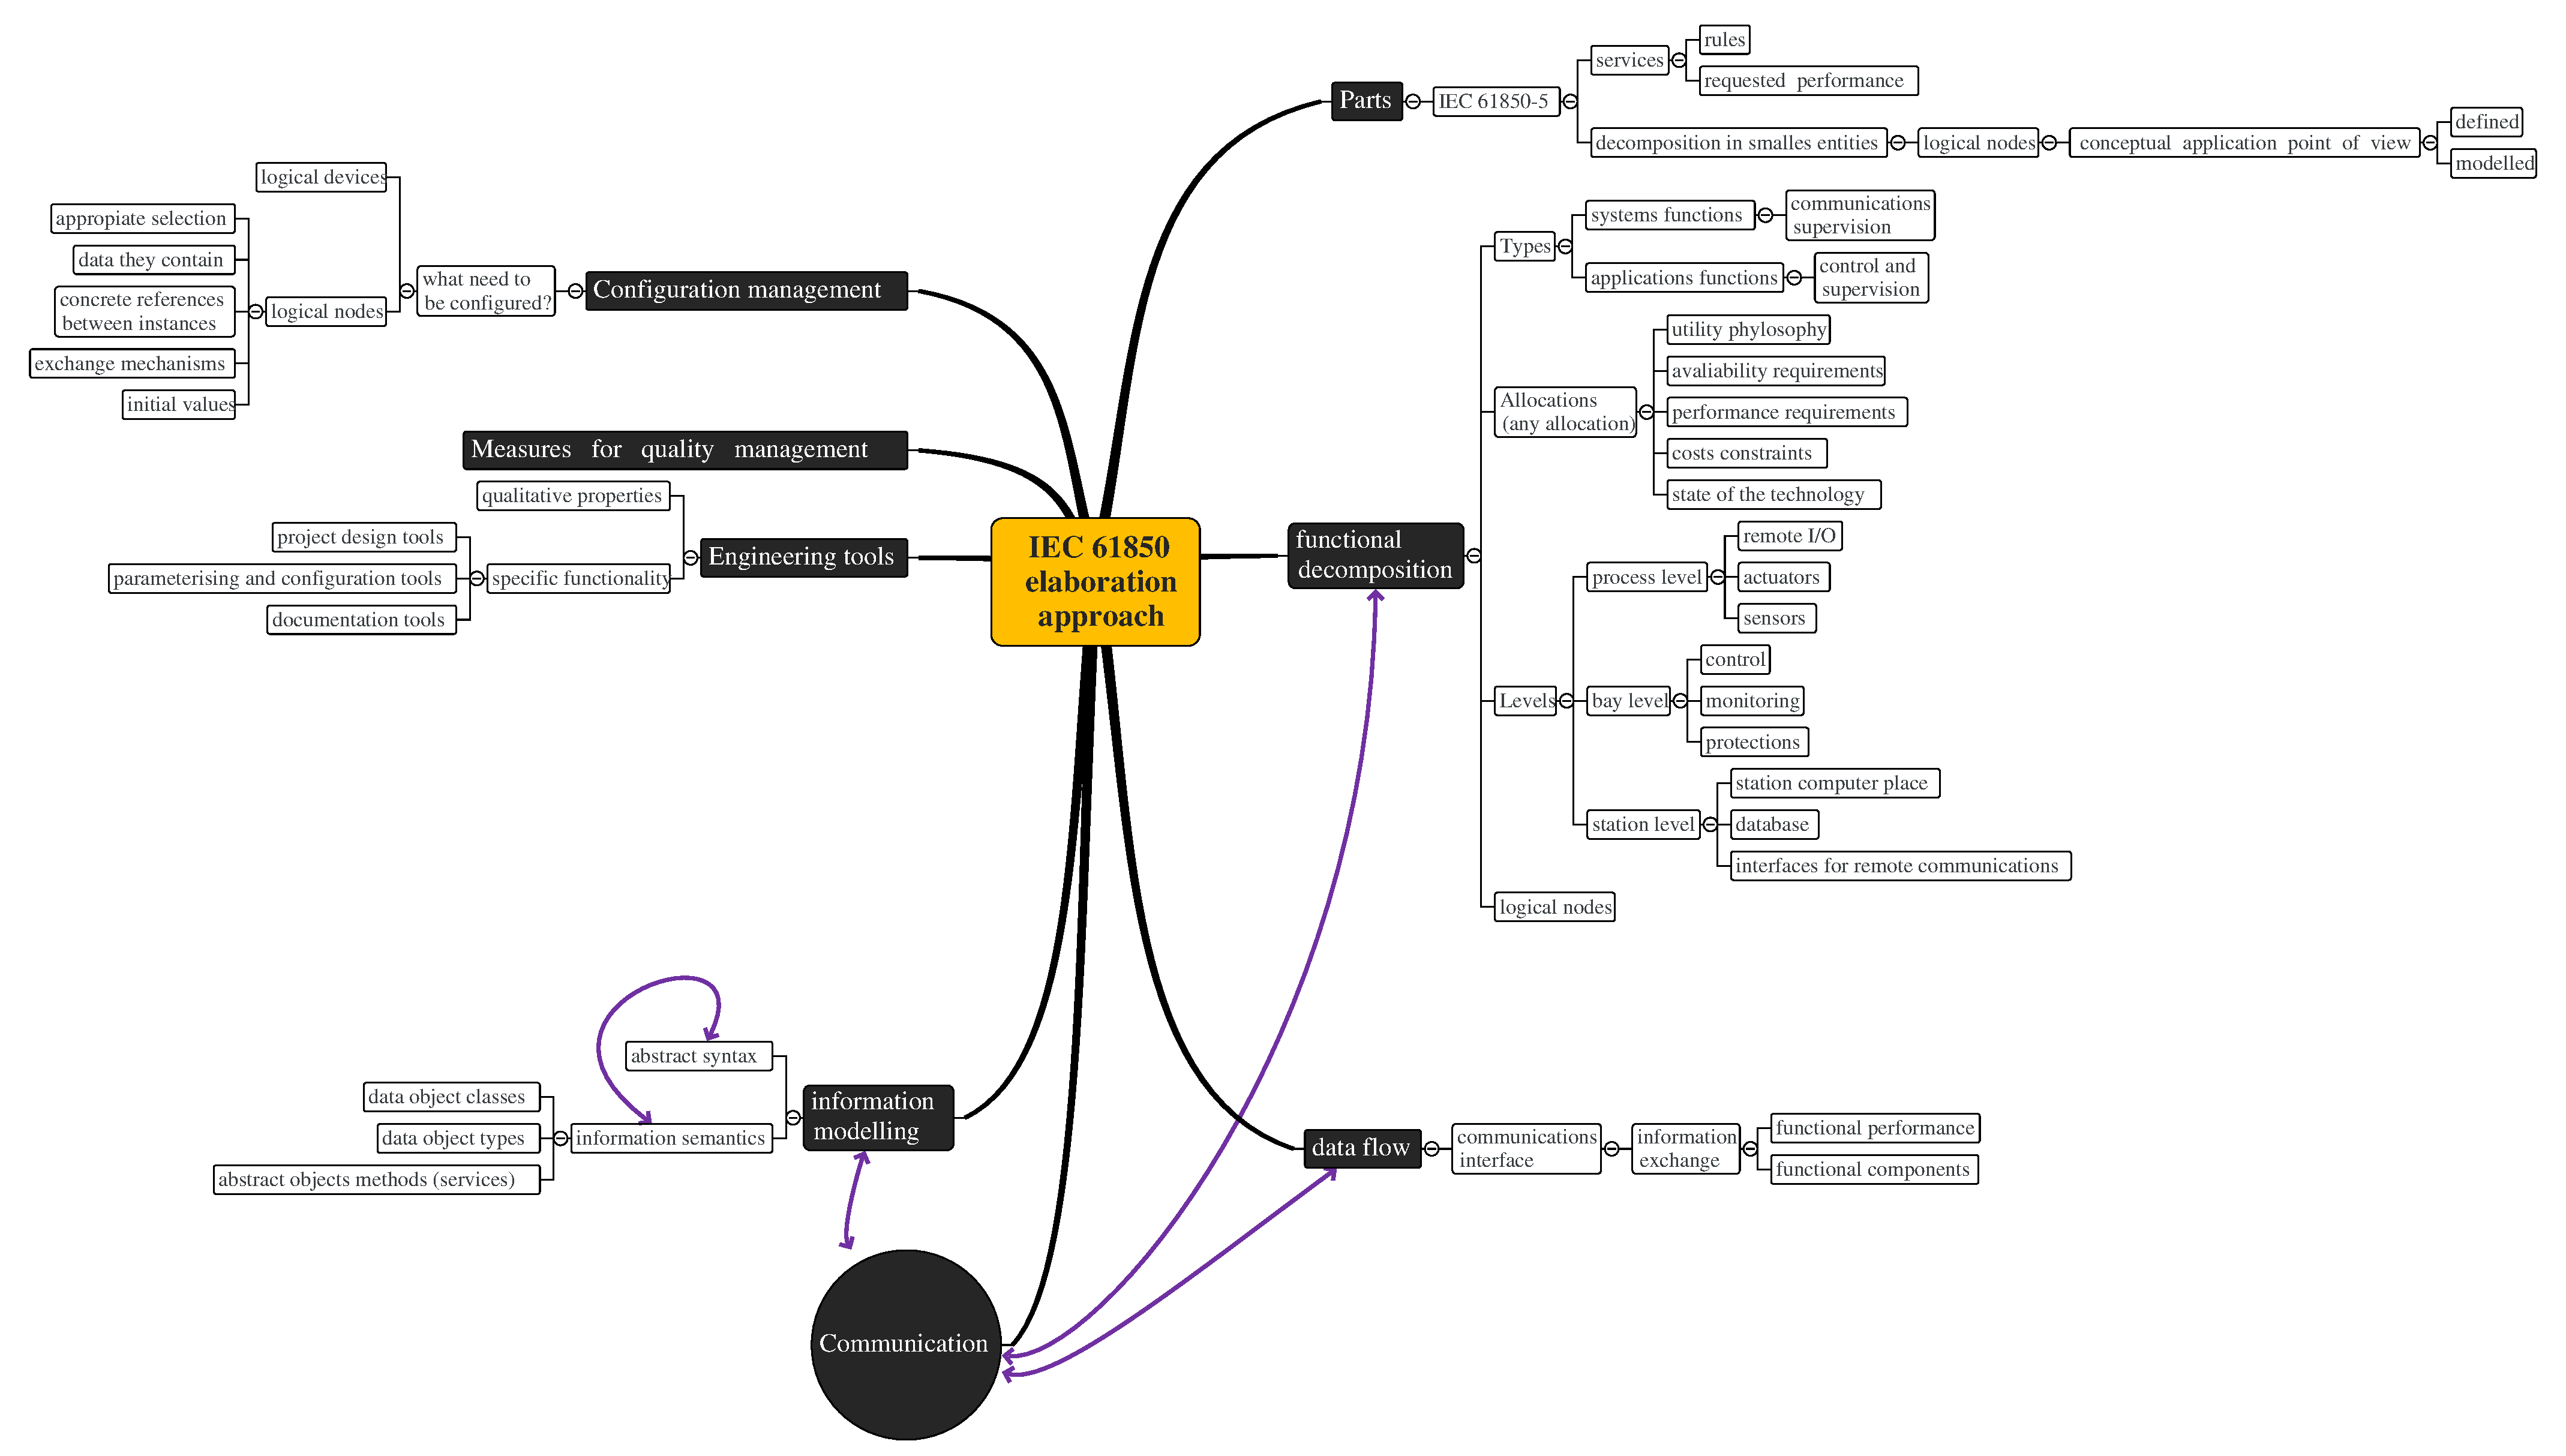
\includegraphics[width=1.0\textwidth]{appendices/IEC61850approach}
  \caption{Borrador - Esquema del futuro capitulo }
  \label{fig:lan-networks-topologies-fig3}
\end{figure}

\begin{figure}
  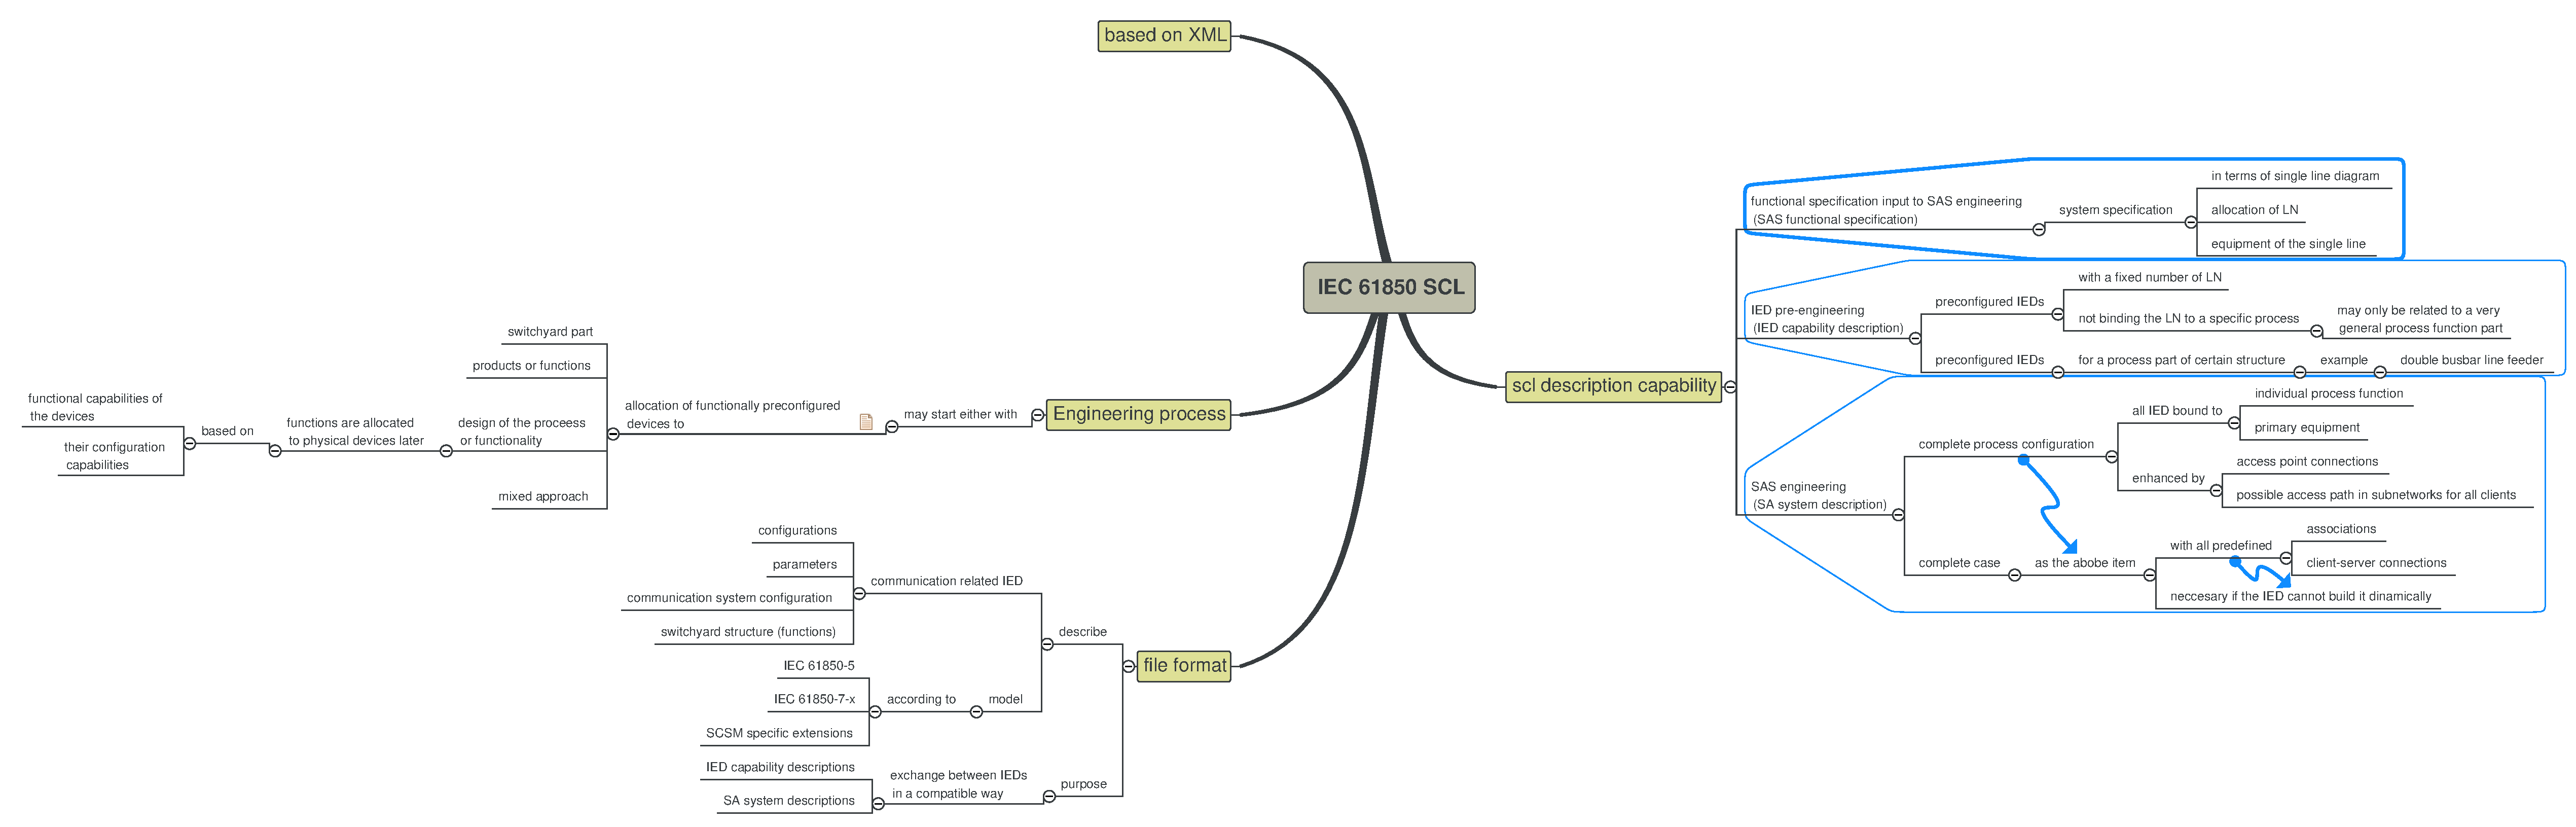
\includegraphics[width=1.0\textwidth]{appendices/IEC61850SCL}
  \caption{Borrador - Esquema del futuro capitulo }
  \label{fig:lan-networks-topologies-fig4}
\end{figure}



%%Este capítulo debe ser el primer tema técnico a tratar,
%%debido a que mi tema se trata al modelado de objetos 
%%y de servicios de comunicación (al final los servicios
%%de comunicación se modelan como objetos via xml)
%%y también la utilización de interfaces da una buena base
%%para entender las capas del modelo OSI: las interfaces
%%que posee cada capa para comunicarse con las otras
%%(servicios) son muy bien compreendidas una vez
%%tratada el tema de interfaces de OOP. Al final, 
%%este tema de interfaces es 
%%abstracción, tratada en ingeniería de software. Por 
%%ello, es un buen punto empezar desde aquí.

\chapter{Object-oriented programming}

\section{Introduction}

The IEC 61850 information model 
is classified as a  
\glsentrytext{O-O} system. Is necessary 
to have a clear understanding of \gls{O-O} technology
to dive into IEC 61850 object modelling. 
For this reason this chapter describes 
the \gls{O-O} technology
on which the IEC 61850 information model 
has been standarized\todo[inline]{No se si esta 
bien escrita la palabra standarized}. 

The chapter does not describe all the \gls{O-O} principles, 
just \todo{�trans:just focuses or focuses just?} focuses 
on the neccesary
background to understand the IEC 61850 
information model. 
The sections which follow will define the 
background which the IEC 61850 
object oriented information system 
was constructed, both formally 
and through examples.
\todo[inline]{debo agregar las abreviaciones de O-O
a mi glossaries package}
A detailed description of the \gls{O-O} fundamentals  
and reference materials are provided. To achieve a 
robust concepts comprehension a practical 
implementation with the%the Unified Modeling Language 
\gls{UML} 
\todo{agregar al glossaries} 
\cite{UML2:2009} 
and Java \cite{Java:specification} are provided. 
This chapter is very
practical in the sense that uses language programmings to model 
very carefully selected models  
used by the IEC 61850 standard, 
(but not explaining explicitly nothing 
about the standard yet!).
This chapter is destined 
for electrical engineers and professionals of 
related areas readers which the \gls{O-O} software construction 
is not part of the curriculum. For this reason, 
the practical examples uses electricity area 
elements. The readers with a strong knowledge 
of programming could skip this
chapter \todo[inline, color=blue!50!red!50]{
	deber\'ia agregar esta ultima frase?:
	\emph{The readers with a strong knowledge 
	of programming could skip this
	chapter}
}




\todo[inline]{En este cap�tulo voy a agregar 
los graficos a continuacion:

(los ejemplos que voy usando son con estas clases)}


\begin{figure}
  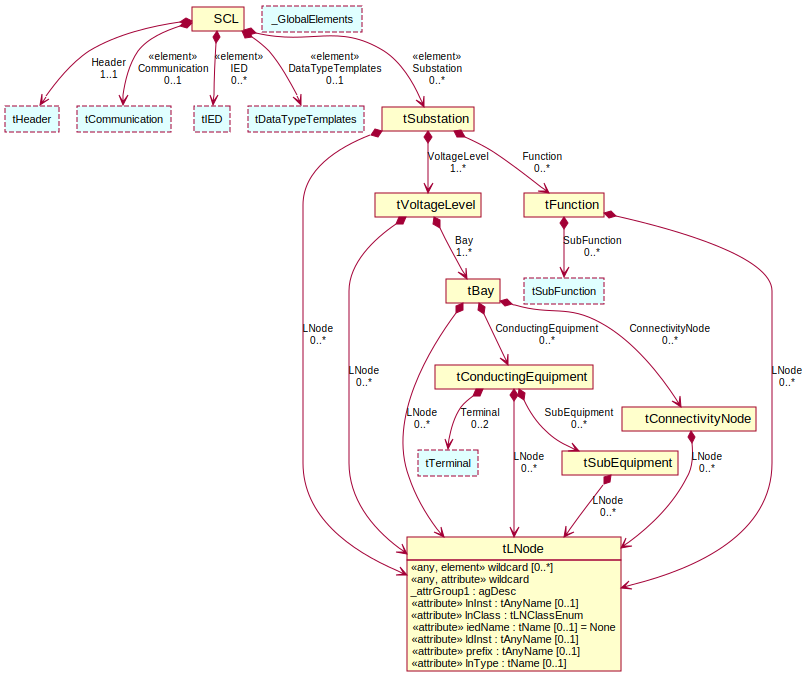
\includegraphics[width=1.0\textwidth]{chapters/ch-oop/figures/LogicalNodeAllocationStructure}
  \caption{Logical Node and their role at the substation level}
  \label{fig:LogicalNodeAllocationStructure}
\end{figure}

\begin{landscape}
	\begin{figure}	
	  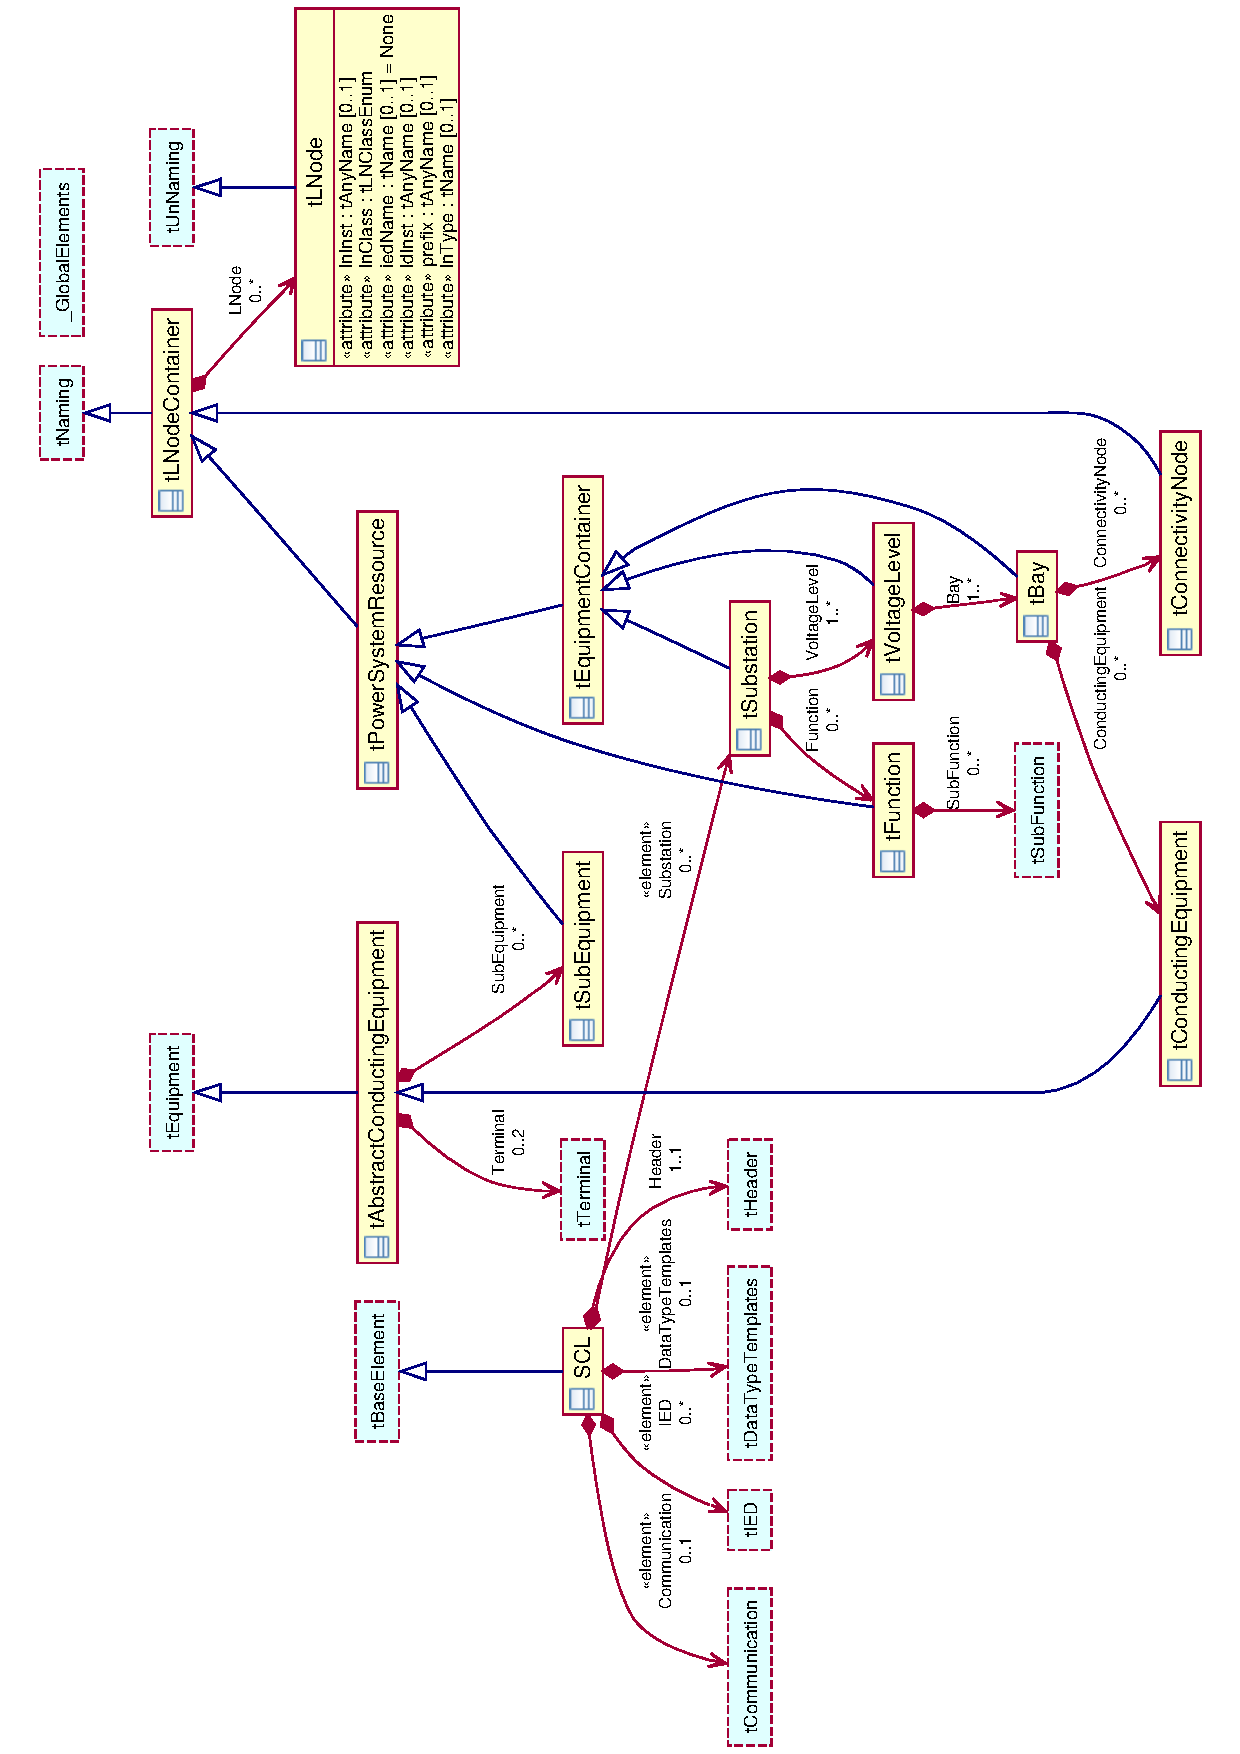
\includegraphics[angle=-90, width=1.0\linewidth]{chapters/ch-oop/figures/LogicalNodeAllocationStructure_with_heritance}
	  \caption{Logical Node and their role at the substation level, depicted with
	  the heritance details}
	  \label{fig:LogicalNodeAllocationStructure_with_heritance}
	\end{figure}
\end{landscape}
	
\section{Basics of object-oriented programming}

\subsection{Introduction to object-oriented programming}

%TODO: citar
%esta parte fue obtenida del libro de adobe, del cap 5. 
Object-oriented programming (OOP) is a way of organizing the code 
in a program by grouping it into objects-individual elements that include 
information (data values) and functionality. Using an 
object-oriented approach to organizing a program allows 
you to group particular pieces of information (for 
example, a automation function or a current value) together with 
common functionality or actions associated with that 
information (such as ``switchgear actuation'' or 
``voltage measurement''). These items are combined into a single 
item, an object (for example, an 
\todo[size=\tiny]{cambiar por un ejemplo el\'ectrico}
``Album'' or ``MusicTrack''). Being 
able to bundle these values and functions together provides several 
benefits, including only needing to keep track of a single 
variable rather than multiple ones, organizing related 
functionality together, and being able to structure 
programs in ways that more closely match the real world.  


\subsection{Common object-oriented programming tasks}

%Aca va la pagina 99 de actionscript programming.
In practice, 
%citar las prácticas comunes
\begin{itemize}
	\item Defining classes
	\item Creating properties, methods, and get and set accessors (accessor
	methods) 
	\item Controlling access to classes, properties, methods, and accessors
	\item Creating static properties and methods
	\item Creating enumeration-like structures
	\item Defining and using interfaces
	\item Working with inheritance, including overriding class elements 
\end{itemize}



\section{Classes}

A class is a static 
%off-line \todo{es realmente off-line?}
template from which objects are 
created. Classes are used 
to classify objects thanks 
that its defines 
common operations 
and a data structure, 
and the types of 
datas that the object can 
store.\\


%Codigo fuente
%C:\Documents and Settings\DELL\Mis
%documentos\tesismayo\tesismayo\thesis\chapters\ch-oop\source\java\src\HelloWorld.java
%\lstinputlisting[label=samplecode,caption=A sample]{sourceCode/HelloWorld.java}
%chapters\ch-oop\source\java\src\HelloWorld.java
\lstinputlisting[label=codeClass,
caption=Class in Java]{chapters/ch-oop/source/java/src/SERVER_v1.java}

%%TODO: cite adobe book

\subsection{Attributes}
\todo[inline]{completar esta parte}
	\lstinputlisting[label=codeAttributes,
	caption=Class with attributes in Java]
	{chapters/ch-oop/source/java/src/SERVER_v2.java}



\subsection{Methods}
Methods are functions that are part of a class 
definition. Once an instance of the class is created, 
a method is bound to that instance.\\
	\lstinputlisting[label=codeMethod,
	caption=Class with attributes and methods in Java]
	{chapters/ch-oop/source/java/src/SERVER_v3.java}



	\subsubsection{Get and set accessor methods}
	Get and set accessor functions, also called getters 
	and setters, allow you to adhere to the programming principles of 
	information hiding and encapsulation while providing an 
	easy-to-use programming interface for the classes that you 
	create. Get and set functions allow you to keep your class 
	properties private to the class, but allow users of your class 
	to access those properties as if they were accessing a 
	class variable instead of calling a class method. 
	The advantage of this approach is that you can avoid 
	having two public-facing functions for each property 
	that allows both read and write access. \\

		\lstinputlisting[label=codeMethod,
		caption=Class with attributes, methods, getters and setters in Java]
		{chapters/ch-oop/source/java/src/SERVER_v4.java}
	
	
	\subsubsection{Constructor methods}
	Constructor methods, sometimes simply called constructors, 
	are functions that share the same name as the class in 
	which they are defined. Any code that you include in 
	a constructor method is executed whenever an instance of the 
	class is created with the  new  keyword. \\

		\lstinputlisting[label=codeMethod,
		caption=Class with attributes, methods, 
		getters, setters and constructors in
		Java] {chapters/ch-oop/source/java/src/SERVER_v5.java}

	
\section{Intefaces}

%\input{chapters/ch-oop/blah blah blah}

\chapter{Computer Networks}

\section{Introduction}

The purpose of this chapter is to provide the necessary background 
 to understand the concepts related to computer networks, 
focusing to explain the main concepts applied to the IEC 61850. 

\section{Transmission technologies}

Types of transmission technology:
\begin{itemize}
  \item Broadcast links.
  \item Point-to-point links.
\end{itemize}

Broadcast networks have a single communication channel 
that is shared by all the machines on the network. 
Short messages, called packets in certain contexts, 
sent by any machine are received by all the others. An 
address field within the packet specifies the intended 
recipient. Upon receiving a packet, a machine checks the 
address field. If the packet is intended for the receiving 
machine, that machine processes the packet; if the 
packet is intended for some other machine, 
it is just ignored. Some broadcast systems also 
support transmission to a subset of the machines, 
something known as multicasting \cite{Tanembaum:2003cn}. 

In contrast, point-to-point networks, sometimes 
called unicasting, consist of
many connections between individual pairs of machines. To go 
from the source to the destination, a packet on this 
type of network may have to first visit one or more 
intermediate machines. Often multiple routes, of 
different lengths, are possible, so finding good 
ones is important in point-to-point 
networks \cite{Tanembaum:2003cn}.


\section{Adressing and routing}

The process of determining systematically how to forward 
messages toward the destination node based on its 
address is called routing. \cite{PetersonDavie:2003}

Adressing types: \\

	\subsection{Unicast}
	The source node wants to send a message to a single destination node.
	
	\subsection{Broadcast}
	The source node want to \emph{broadcast} a message to all the 
	nodes on the network.
	
	\subsection{Multicast}
	The source node send a message to some subset of the 
	other nodes, but not all of them.
	

	
	
	

\section{Local Area Networks}
Local area networks, generally called LANs, are privately-owned 
networks within a single building or campus of 
up to a few kilometers in size. LANs are 
distinguished from other kinds of networks by three  
characteristics:
  
\begin{itemize}
  \item their size, 
  \item their transmission technology, and
  \item their topology.  
\end{itemize}

LANs are restricted in size,  which means that the 
worst-case transmission time is bounded and known in 
advance. Knowing this bound makes it possible to use 
certain kinds of designs that would not otherwise 
be possible. It also simplifies network management. 
LANs may use a transmission technology consisting 
of a ¿¿¿¿¿¿¿cable??????? to which all the machines 
are attached. Traditional  LANs  run  at  
speeds  of  10  Mbps  to  100 
Mbps, have low delay (microseconds or nanoseconds), 
and make very few errors. Newer LANs operate at up to 
10 Gbps. 

Various topologies are possible for broadcast LANs. 
Figure \ref{fig:lan-networks-topologies-fig} shows 
two of them. In a 
bus (i.e., a linear cable) network, 
at any instant at most one machine is the master 
and is allowed to transmit. All other machines are 
required to refrain from sending. An arbitration 
mechanism is needed to resolve conflicts when two or more 
machines want to transmit simultaneously. The 
arbitration mechanism may be centralized or 
distributed. IEEE 802.3, popularly called Ethernet, 
for example, is a bus-based broadcast network with 
decentralized control, usually operating at 10 Mbps 
to 10 Gbps. Computers on an Ethernet can transmit 
whenever they want to; if two or more packets collide, 
each computer just waits a random time and tries again later. 


\begin{figure}
  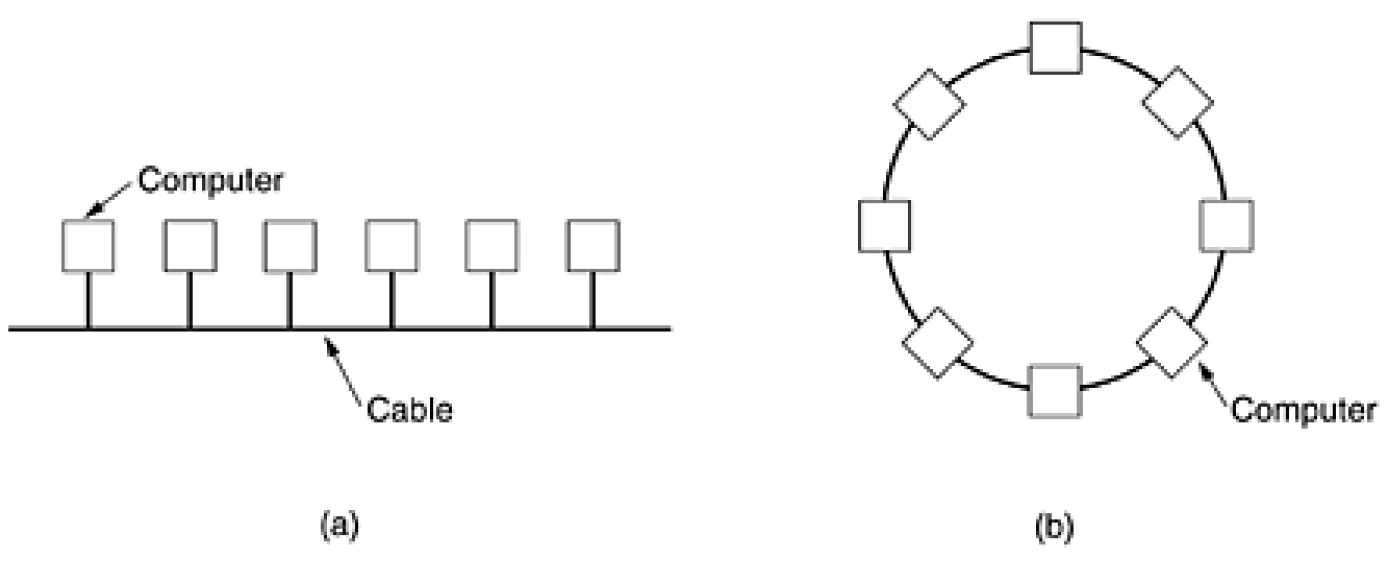
\includegraphics[width=1.0\textwidth]{chapters/ch-networks/figures/lan-networks-topologies}
  \caption{Two broadcast networks. (a) Bus. (b) Ring \cite{Tanembaum:2003cn}}
  \label{fig:lan-networks-topologies-fig}
\end{figure}

\section{Annotations}



\chapter{IEC 61850 Overview}

\section{Objects for distributed systems}

The effective distribution of Logical Nodes 
on diferents IEDs  
is a reality thanks to researches about 
the structure of distributed systems. More 
than 20 years ago emerged requirements 
for the object paradigm to suport the 
design and development of distributed systems.

Theses quotes were extracted from Jazayeri 
1988 research:

\emph{
``An object on one node can send a (multicast) message 
to several other objects \ldots''
} (MCAA) \todo{completar y ver si esta bien}

\emph{
`` \ldots The ability to group 
a set of objects and address them as one entity 
is important in many applications both from an 
efficiency point of view and from a program 
structuring point of view \ldots'' 
} (DO, DATA-SET, FCD, FCDA)\todo{completar y ver si esta bien}

\emph{
`` \ldots a final 
difference is that our objects are active and 
not reactive, in the sense that they can start 
up spontaneosly performing operations, not 
necessarily only in response to method invocations.
Such a facility is useful, for example, to allow objects 
to monitor the enviroment and change their behavior based 
on changes in the enviroment \ldots'' 
} (Some active objects 
are GOOSE, URCB and some passive object 
are \todo{completar y ver si esta bien})

\cite{Jazayeri:1988}.



\begin{figure}
  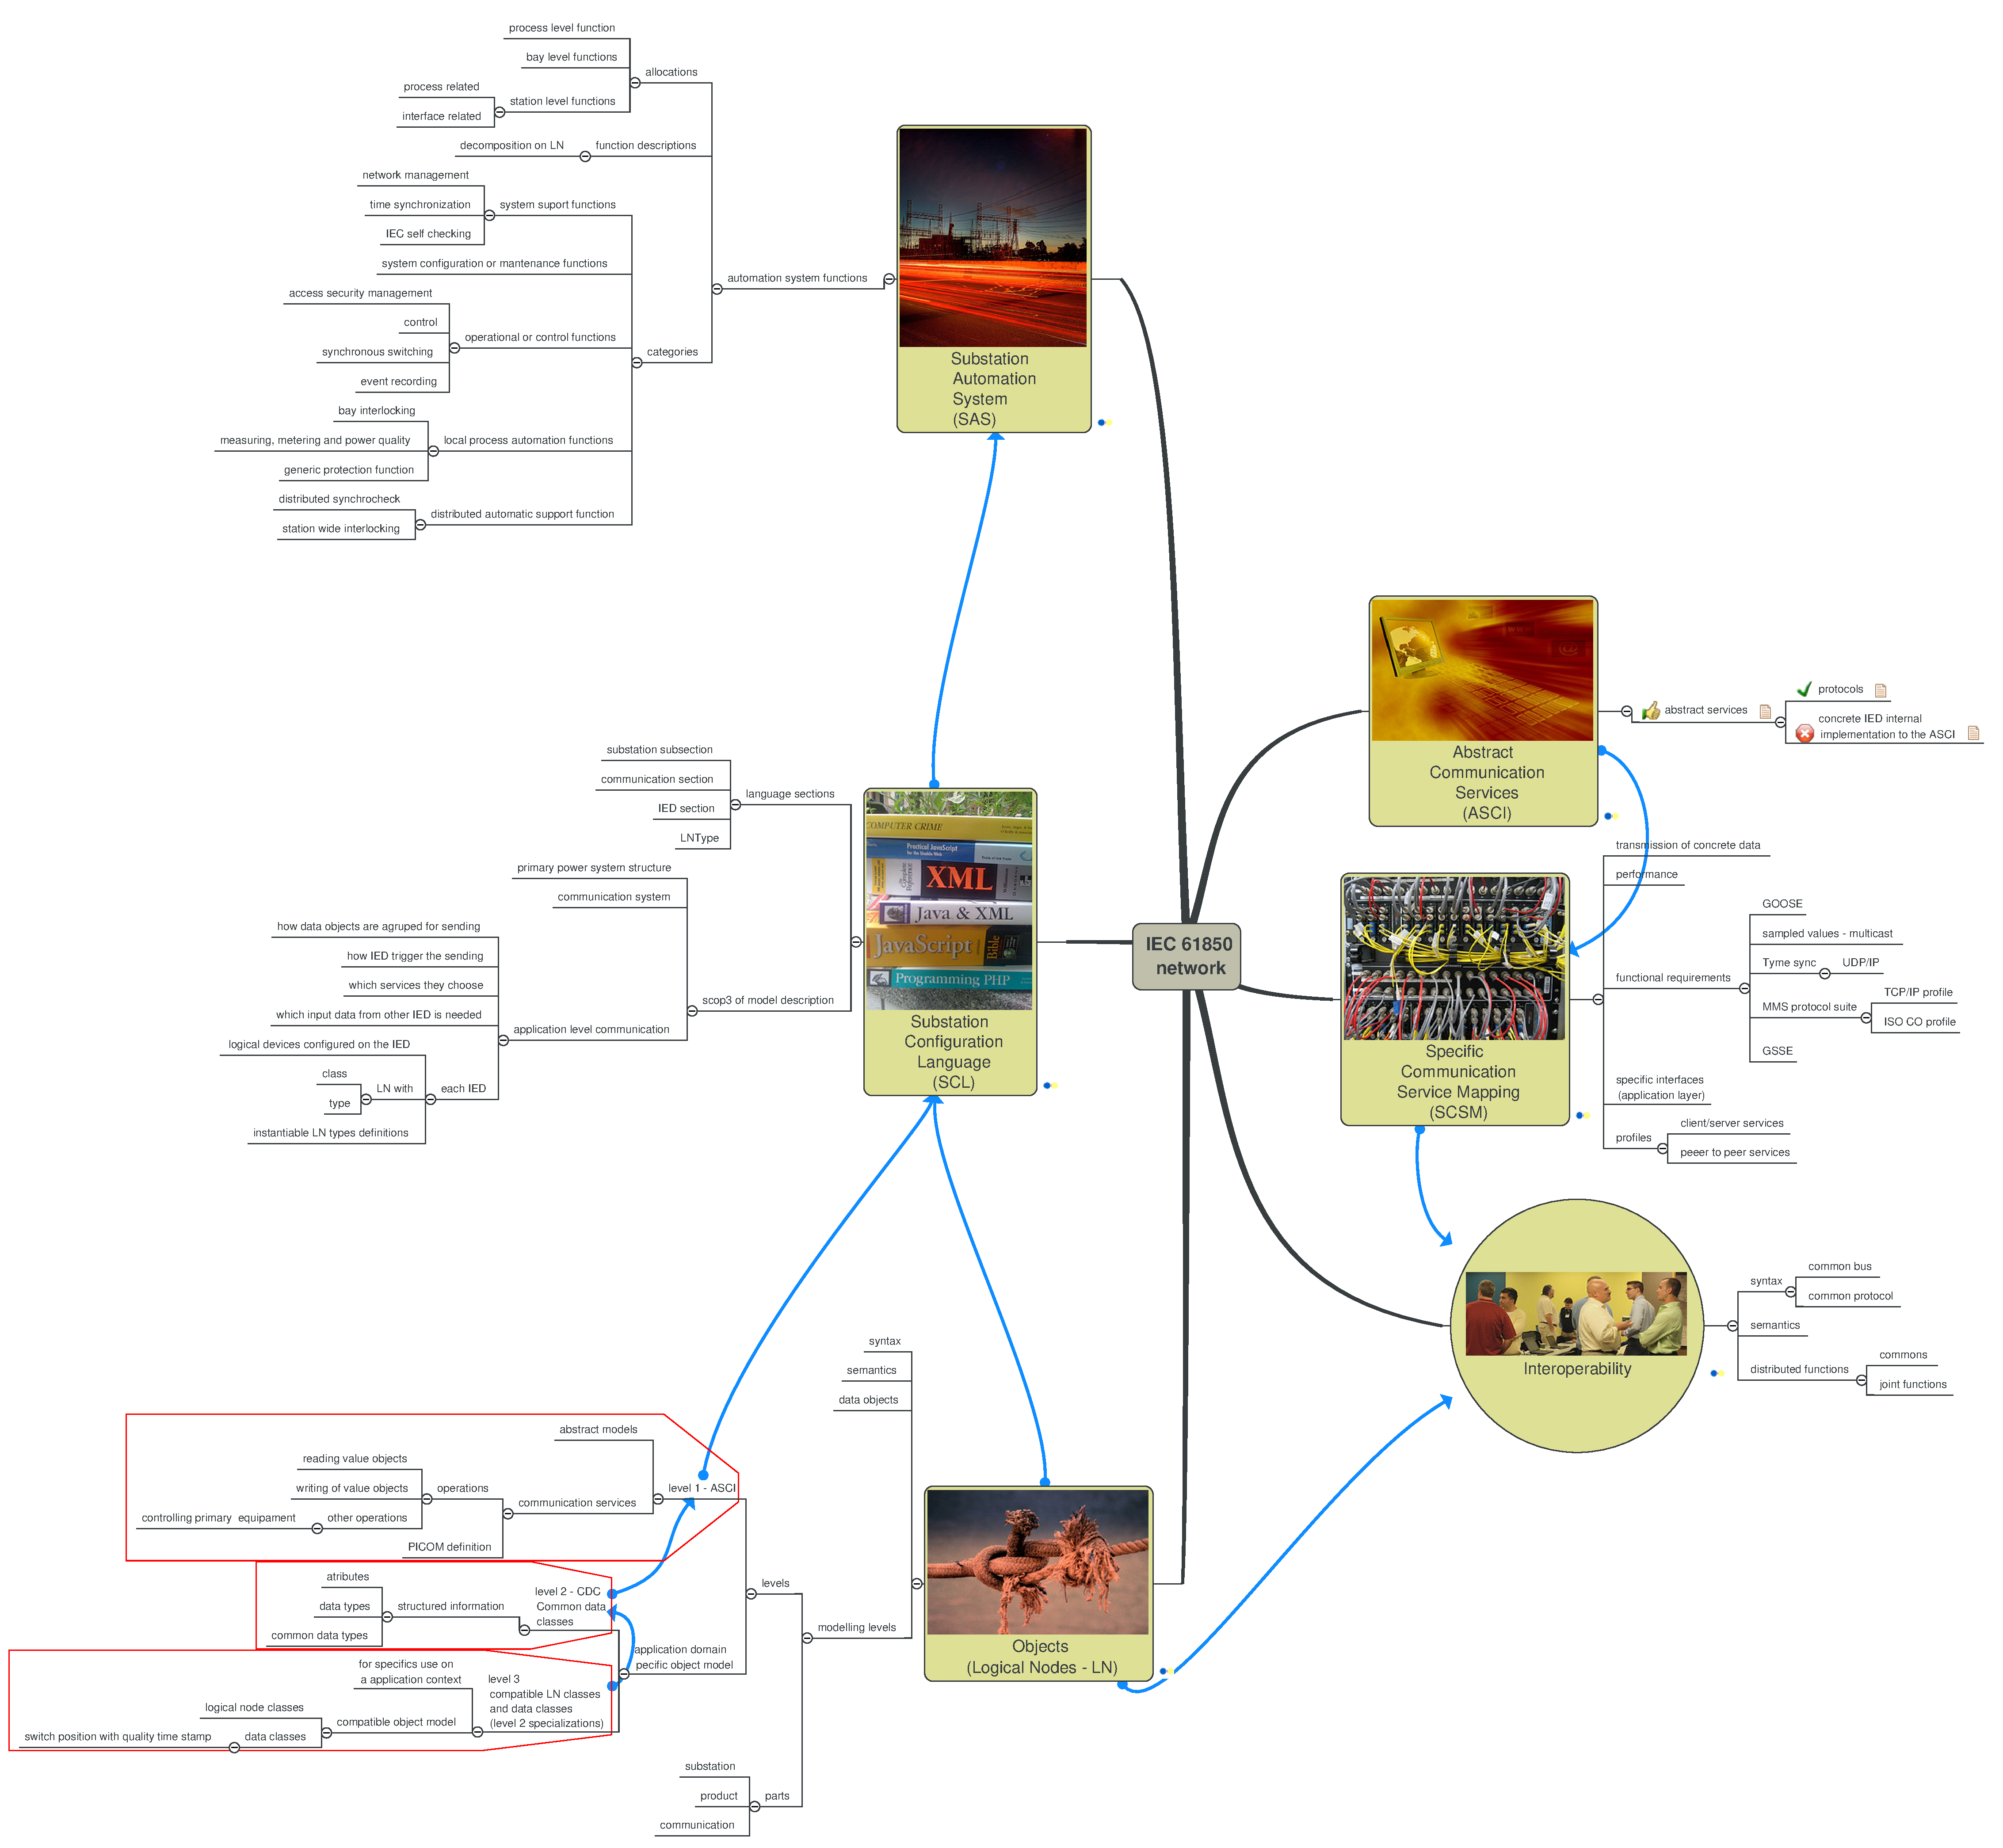
\includegraphics[width=1.0\textwidth]{appendices/IEC61850network}
  \caption{Borrador - Parte del esquema del futuro capitulo }
  \label{fig:lan-networks-topologies-fig1}
\end{figure}

\begin{landscape}
	\begin{figure}
	  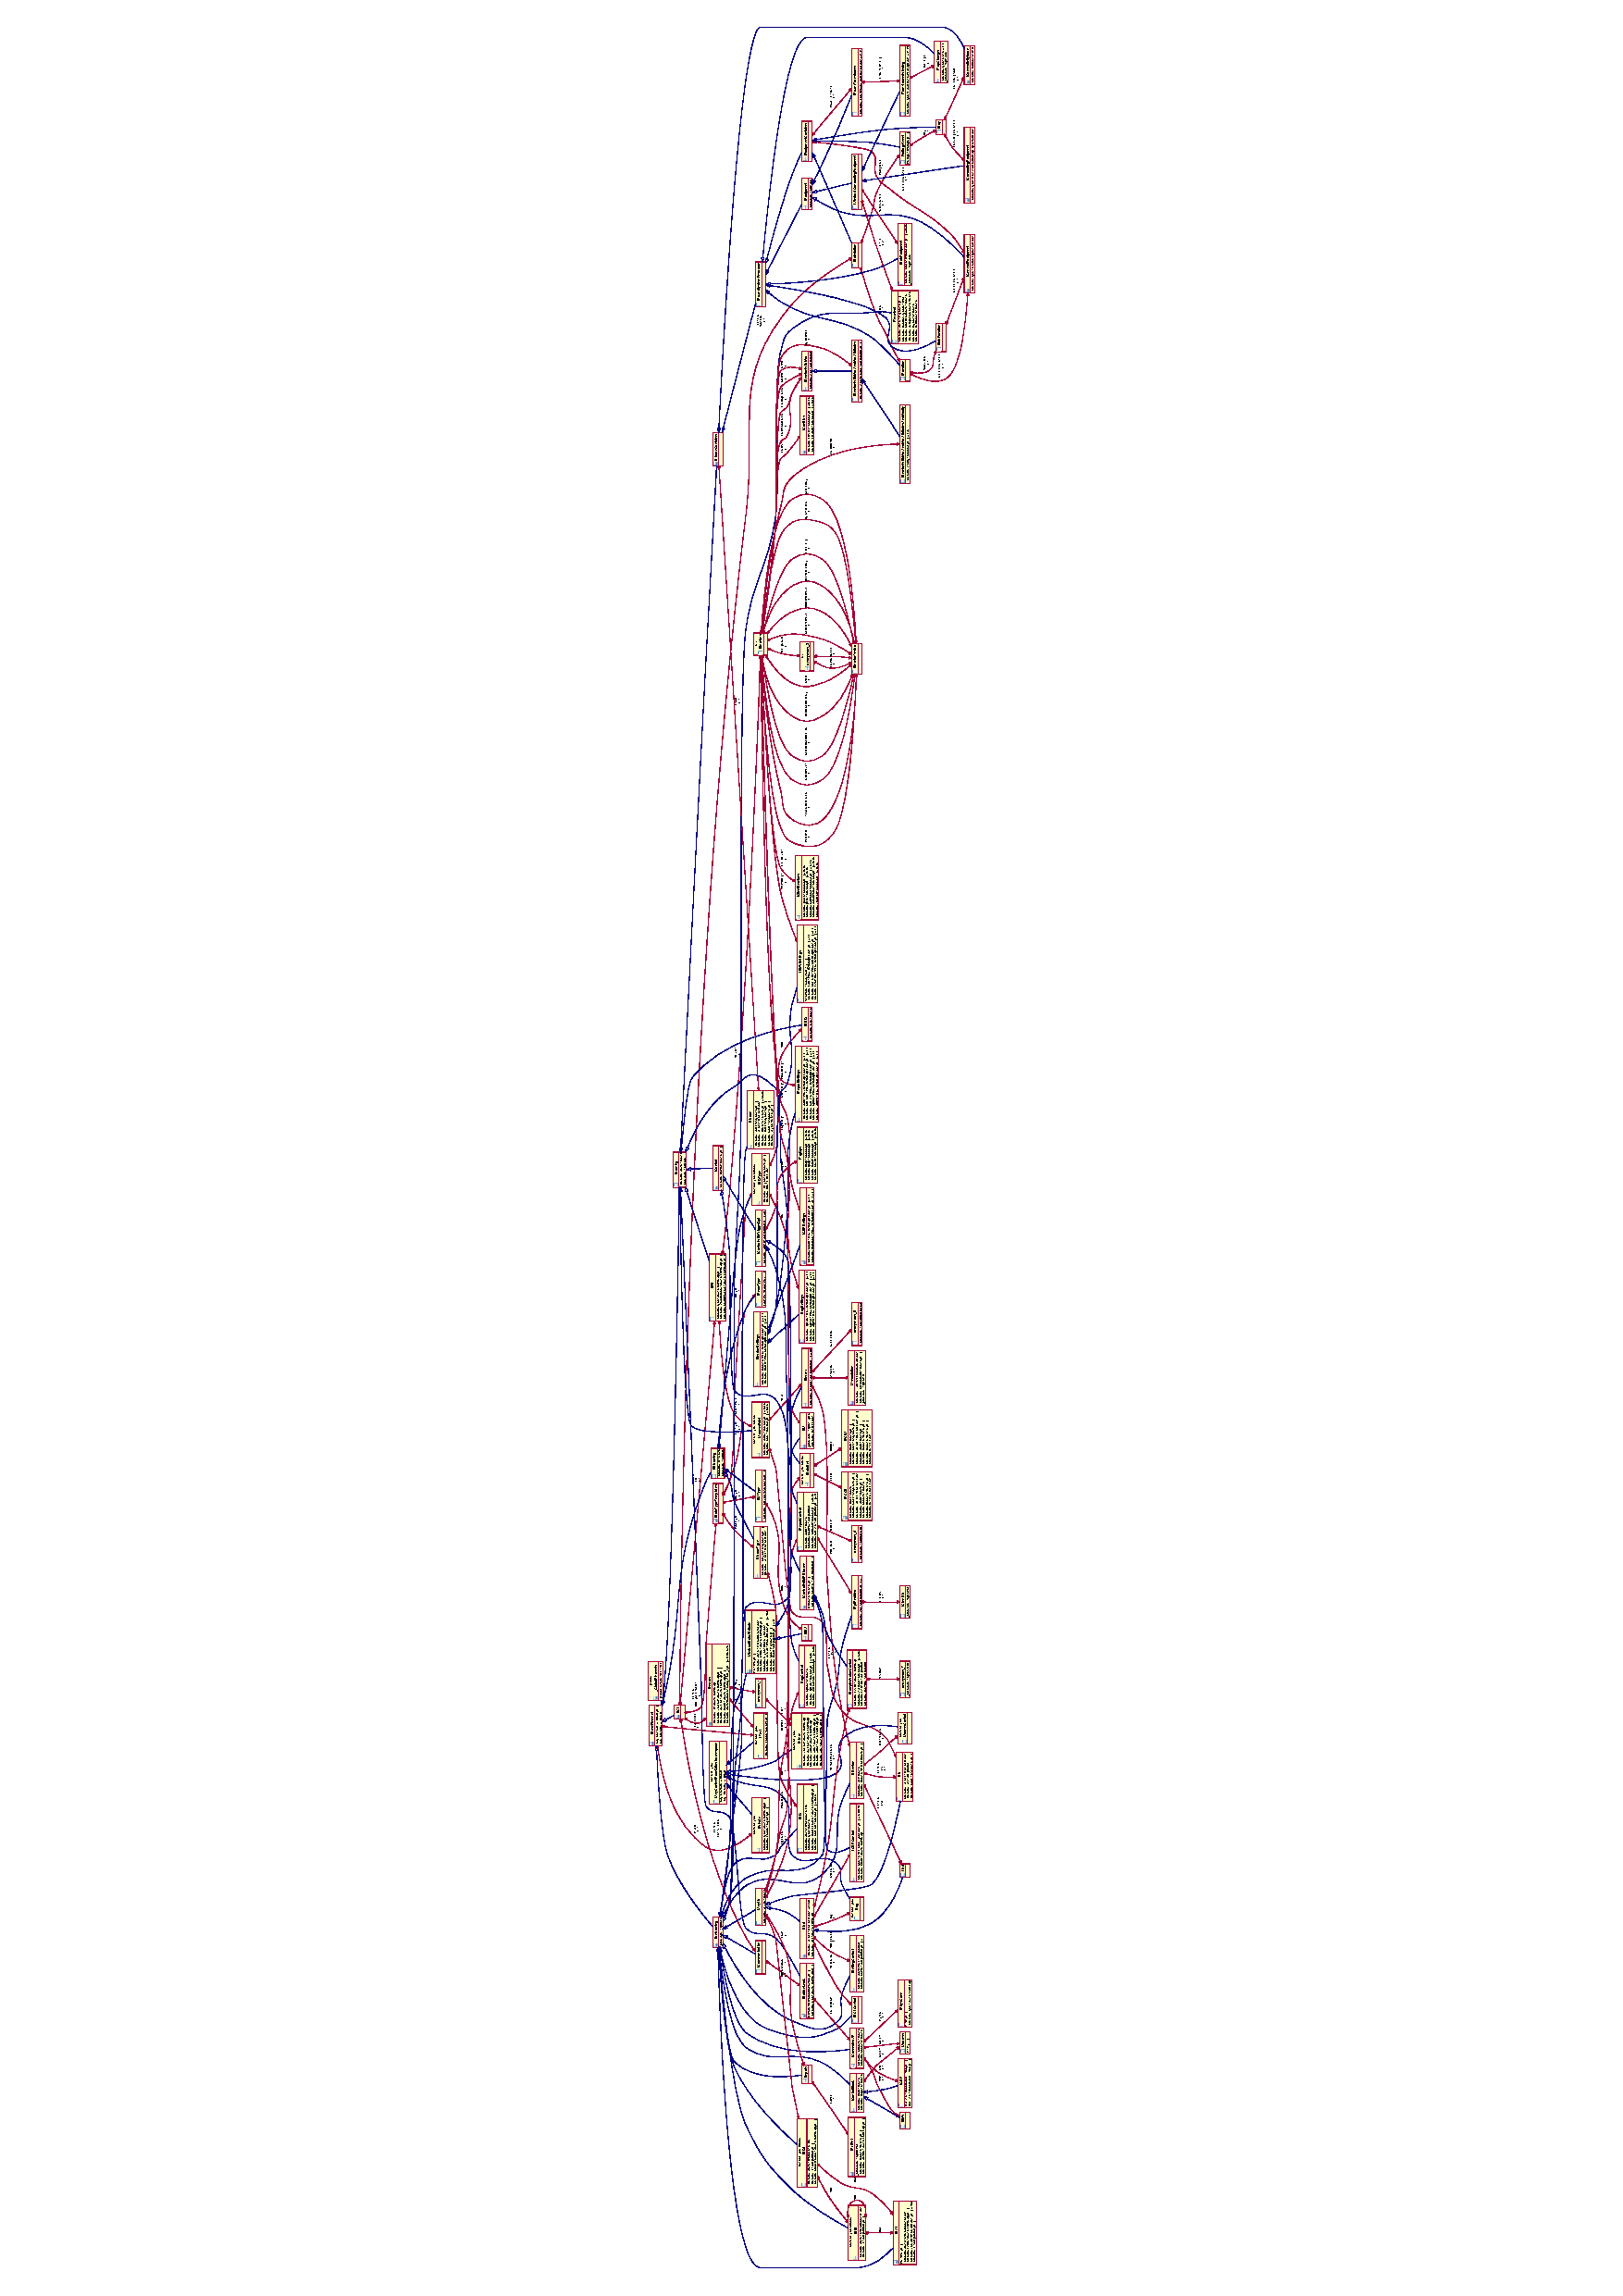
\includegraphics[angle=-90, width=1.0\linewidth]{appendices/JavaPrinting}
	  \caption{Borrador - Parte del esquema del futuro capitulo }
	  \label{fig:lan-networks-topologies-fig2}
	\end{figure}
\end{landscape}
 




%\chapter{Theoretical Foundations}

% measurement of spin observables is challenging but rewarding
%   examples?
% 

\section{The Simple Parton Model}

% predates QCD, invented to explain scaling of F_{1,2}
% Leader cites 69 Feynman PRL as inventor of parton model, but I skimmed the Letter and I don't see it.
% \cite{Panofsky:1968pb} -- confirmation of Bjorken scaling
% \cite{Bjorken:1968dy} -- Bjorken scaling

In the late nineteen-sixties high energy physicists at SLAC confirmed Bjorken's
hypothesis that the inelastic structure functions of the proton scaled; that is,
at high energies they did not depend on the $Q^2$ of the interaction. This
result stood in sharp contrast to the power-law behavior of the proton's elastic
form factors, and implied the existence of point-like constituents inside the
proton. These ``partons'' were conceived as effectively massless,
electromagnetically charged particles; in the deep-inelastic scattering
(DIS) regime, a virtual photon interacts with a parton, not the proton as a
whole.

Scaling is manifest when Bjorken's $F_1$ structure function is expressed in terms of the number densities $q(x)$ of quarks and $\bar q(x)$ of antiquarks as
%
\begin{equation}
  F_1(x, Q^2) = \frac{1}{2}\sum_{j}{e_j^2[q_j(x) + \bar{q}_j(x)]}
\end{equation}
%
where the sum is taken over quark flavors $j$ and $e_j$ is the electromagnetic charge of flavor $j$.  In longitudinally polarized DIS we define an analogous polarization density $\Delta  q(x) \equiv q_+(x) - q_-(x)$ as the difference in number density between quarks whose spins are aligned with the (longitudinal) spin of the proton and quarks whose spins are anti-aligned; the polarized analogue to $F_1$ is then
%
\begin{equation}
  g_1(x, Q^2) = \frac{1}{2}\sum_{j}{e_j^2[\Delta q_j(x) + \Delta \bar{q}_j(x)]}.
\end{equation}

In the na\"ive parton model we assume $SU(3)_F$ flavor symmetry and thus it is useful to rewrite the expression for $g_1$ in terms of quantities which have specific $SU(3)_F$ transformation properties:
%
\begin{equation}
  g_1(x) = \frac{1}{9}[\frac{3}{4}\Delta q_3(x) + \frac{1}{4}\Delta q_8(x) + \Delta \Sigma(x)]
  \label{eqn:g1}
\end{equation}
%
where
%
\begin{eqnarray}
  \Delta q_3(x) & = & (\Delta u + \Delta \bar{u})_x - (\Delta d + \Delta \bar{d})_x \nonumber \\
  \Delta q_8(x) & = & (\Delta u + \Delta \bar{u})_x + (\Delta d + \Delta \bar{d})_x - 2(\Delta s + \Delta \bar{s})_x \nonumber \\
  \Delta \Sigma(x) & = & (\Delta u + \Delta \bar{u})_x + (\Delta d + \Delta \bar{d})_x + (\Delta s + \Delta \bar{s})_x
  \label{eqn:su3_dis}
\end{eqnarray}
%
The first moments of these quantities are the hadronic matrix elements of an octet of quark $SU(3)_F$ axial-vector currents $J_{5\mu}^i$ and a flavor singlet singlet axial current $J_{5\mu}^0$.  In the limit of massless partons the non-singlet currents are scale-independent quantities, and are known from $\beta$-decay measurements \cite{}:
%
\begin{eqnarray}
  a_3 & = & \int_0^1 dx~\Delta q_3(x) = g_A = 1.2670 \pm 0.0035 \nonumber \\
  a_8 & = & \int_0^1 dx~\Delta q_8(x) = 0.585 \pm 0.025
  \label{eqn:beta-decay}
\end{eqnarray} % might be missing a 1/\sqrt{3} in a_8
%
A measurement of the first moment of $g_1^p$ could thus be interpreted as a measurement of the singlet current $a_0 = \int_0^1 dx~\Delta \Sigma (x)$, and in turn as a measurement of the quark spin contribution to the spin of the proton.  We rearrange \ref{eqn:su3_dis} to yield an expression for the singlet current in terms of $a_8$ and the polarized strange quark densities:
%
\begin{equation}
  \Delta \Sigma = a_8 + 3 \int_0^1 dx~(\Delta s + \Delta \bar s)
  \label{eqn:a_0_prediction}
\end{equation}
%
If one assumes that the sea quark distribution is either unpolarized or CP-symmetric and thus does not contribute to the spin of the proton, Equation \ref{eqn:a_0_prediction} becomes a \textit{prediction} for $\langle S_z \rangle$, as noted by Ellis and Jaffe \cite{Ellis:1973kp} in 1974.

% Should say something about the Sehgal result \cite{Sehgal:1974rz} that concludes the quark contribution to the spin of the proton is $\sim$ 0.3, in agreement with Ellis-Jaffe but using a slightly different derivation (Bjorken sum rule \cite{Bjorken:1966jh}, equivalent parton model result (cites several people), use SU(3) symmetry to obtain same result for $\Xi^- (dss) \rightarrow \Xi^0 (uss) + e + \bar \nu_e$, expresses $\frac{G_A}{G_V}$ ratios in terms of experimentally-measurable quantities $F$ and $D$ (calls that step the octet-model results), seems that $F+D = \frac{G_A}{G_V} \approx g_A = a_3$, F/D 

% In much of the literature I see $g_A$ instead of Griffiths' $\frac{G_A}{G_V}$.  I wonder if that is a definition, or if the literature just takes the Conserved Vector Current hypothesis $G_V = 1$ for granted? -- yes, it's the latter, see Stiegler 1995

% \begin{equation}
%   \Gamma_1^p \equiv \int_0^1 dx~g_1(x) = \frac{1}{9}[\frac{3}{4}a_3 + \frac{1}{4}a_8 + a_0]
% \end{equation}

% \begin{eqnarray*}
%   a_3 \equiv g_A & = & 1.2670 \pm 0.0035 \\
%   a_8 & = & 0.585 \pm 0.025
% \end{eqnarray*}

\section{First Experimental Tests}

In polarized deep inelastic scattering, a longitudinally polarized lepton beam
is scattered off of nucleon targets polarized parallel or perpendicular to the
beam axis. Asymmetries are formed by comparing event rates for scattering in
different spin configurations. For a spin $\frac{1}{2}$ target, the
asymmetries of interest are

% Stiegler does not include the 1/2 nor the differential in this equation
\begin{equation}
  A_{\parallel} = \frac{d\sigma^{\rightarrow \Leftarrow} - d\sigma^{\rightarrow \Rightarrow}}{2d\sigma_{unpol}}, ~~~~~~~
  A_{\perp} = \frac{d\sigma^{\rightarrow \Uparrow} - d\sigma^{\rightarrow \Downarrow}}{2d\sigma_{unpol}}
\end{equation}

Spin-dependent cross sections can be calculated by contracting the elastic
Compton amplitude $T_{\mu \nu}$ with the photon polarization vectors; in the
presence of parity conservation and time reversal, four of these are
independent \cite{}:
%
\begin{eqnarray}
  \sigma_{1/2} & = & F_1 + g_1 - \gamma^2 g_2, \nonumber \\
  \sigma_{3/2} & = & F_1 - g_1 + \gamma^2 g_2, \nonumber \\
  \sigma_L & = & -F_1 + F_2(1+\gamma^2)/(2x),  \nonumber \\
  \sigma_{TL} & = & \sqrt{2}\gamma (g_1+g_2).
\end{eqnarray}
%
Here $\gamma^2 = Q^2/v^2$. These four cross sections are commonly rearranged
into a pair of virtual photon asymmetries $A_1$ and $A_2$:
%
\begin{equation}
  A_1 = \frac{\sigma_{1/2} - \sigma_{3/2}}{\sigma_{1/2} + \sigma_{3/2}}, ~~~~ A_2 = \frac{\sigma_{TL}}{\sigma_T}
\end{equation}
%
The longitudinal and transverse DIS asymmetries can then be written in terms
of these virtual photon asymmetries. In the case of $A_{\parallel}$ we have
\begin{equation}
  A_{\parallel} = D(A_1 + \eta A_2),
\end{equation}
%
where the coefficients $D$ and $\eta$ can be approximated to first order in
$\gamma$ in terms of the usual DIS kinematic variables and $R =
\frac{\sigma_{L}}{\sigma_T}$:
% include coeffs for A_perp here too?
% Detailed derivation of these results can be found in \cite{Anselmino:1994gn}
\begin{equation}
  D \approx \frac{y(2-y)}{y^2 + 2(1-y)(1+R)}, ~~~~~~~~ \eta \approx \frac{2(1-y)}{y(2-y)} \frac{\sqrt{Q^2}}{E}.
\end{equation}
%
(Similar equations exist for $A_{\perp}$, such that a measurement of both
asymmetries allows an extraction of both $A_1$ and $A_2$). $D$ can be thought
of as a depolarization factor arising from the fact that the photon is not
fully aligned with the lepton beam, and $\eta$ is a kinematic factor that is
usually small. Finally, the polarized structure functions can be written in
terms of $A_{1,2}$:
\begin{equation}
  g_1 = \frac{F_2}{2x(1+R)}(A_1+\gamma A_2), ~~~~~ g_2 = \frac{F_2}{2x(1+R)}(A_2/\gamma - A_1).
\end{equation}
Thus, measurements of $A_{\parallel}$, $A_{\perp}$, $F_2$, and $R$ are
sufficient to extract the polarized structure functions of the nucleon.

% note that they just measured A_parallel and placed a limit on the A_2 contribution
The first DIS experiments to extract $g_1$ using this methodology were E80 and
E130, conducted in the late 1970s and early 1980s at SLAC. These experiments
scattered longitudinally polarized electron beams off of longitudinally
polarized proton targets and were able to measure $A_{\parallel}^p$ in the
range $0.1 < x < 0.7$. Using the positivity limit $A_2 < \sqrt{R}$ they
determined that $A_{\parallel}/D$ was a good approximation for $A_1$, and
after exploiting that assumption their results were consistent with
expectations from the parton model \cite{Alguard:1976bm, Baum:1983ha}.
% there are 2-3 more result papers cited in Baum:1983ha if I want them

In 1988, the European Muon Collaboration (EMC) published data on asymmetries
of longitudinally polarized muon beams scattering off of longitudinally
polarized proton targets. The EMC experiment boasted kinematic coverage down
to $x = 0.01$, an order of magnitude lower than the earlier SLAC experiments,
and the Collaboration extracted measurements of the proton's $g_1$ structure
function using the same assumption that $A_1 \approx A_{\parallel}/D$. The EMC
data on $A_1$ were consistent with the results from SLAC in their overlapping
kinematic regime, but at low $x$ the EMC results deviated significantly from
parton model predictions. As shown in Figure \ref{fig:emc-g1p}, the integral
value of $g_1^p$ obtained from the EMC extraction was incompatible with the
prediction from Ellis and Jaffe. Applying the Bjorken sum rule to obtain a
(significantly negative) value for the integral of $g_1^n$, EMC quoted the
following quark spin contribution to the spin of the proton
\cite{Ashman:1987hv}: % Ashman:1989ig might be the authoritative source
%
\begin{equation}
  \langle S_z \rangle_{u+d} = 0.068 \pm 0.047 \pm 0.103.
\end{equation}
%
This result sparked what was once termed a ``spin crisis'' in particle
physics. Sucessive polarized DIS experiments at CERN, SLAC, and DESY confirmed
and refined the EMC measurement of $g_1^p$ with improved precision over a
wider kinematic range \cite{Adams:1994zd}, and measured both $g_1^n$
\cite{Anthony:1993uf} and $g_1^d$ \cite{Adeva:1993km} which allowed a
verification of the critical Bjorken sum rule.

\begin{figure}
  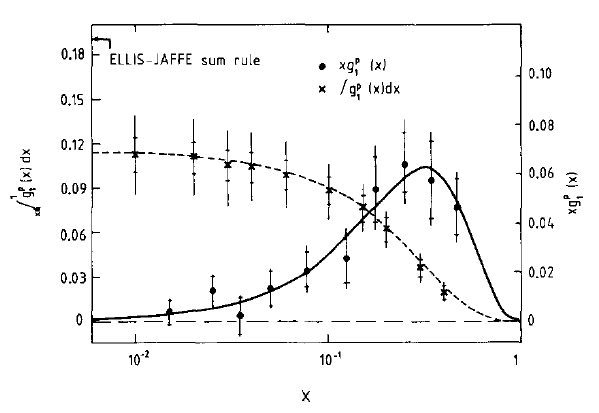
\includegraphics[width=1.0\textwidth]{figures/emc-g1p}
  \caption{EMC extraction of $g^1_p$ and its integral compared to the prediction from Ellis-Jaffe \cite{Ashman:1987hv}}
  \label{fig:emc-g1p}
\end{figure}

Even in that context, the EMC result was surprising. Applying the Bjorken sum
rule to obtain $\int g_1^n$ and again assuming an unpolarized sea, one can
solve for the individual quark spin contributions to the spin of the proton:

\begin{equation}
  \int_0^1 dx~g_1^p(x,Q^2) - g_1^n(x,Q^2) = \frac{g_A}{6}(1 + O(\alpha_s))
\end{equation}

% Rearranging \ref{eqn:g1} to solve for $\Delta \Sigma$ and plugging in values from \ref{eqn:beta-decay} and EMC one finds
% 
% \begin{equation}
%   \Delta \Sigma = 9\Gamma_1^p - \frac{3}{4}a_3 - \frac{1}{4}a_8 = 
% \end{equation}
% 
%   The data covered a sufficient range
% EMC measures first moment of g1, taking a3 and a8 from beta-decay measurements means that we can extract a0 from $\Gamma_1^p$ and it's $\sim$ 0.  But
% 
% \begin{equation}
%   a_0 = \Delta \Sigma = a_8 + 3(\Delta s + \Delta \bar{s})
% \end{equation}
% 
% from above, and if you ignore strange quark contributions (Ellis-Jaffe) you get $a_0 \sim 0.59$, obviously in stark contrast to EMC.  This is the original ``spin crisis''.  And of course $a_0 = 2<S_z^{quarks}>$.
% 
% Any need to mention ``Cloudy Bag'' model here?  I think not.
% 
% 
% \begin{equation}
%   y \equiv \frac{\nu}{E} = \frac{P \cdot q}{P \cdot k}
% \end{equation}
% 
% \begin{equation}
%   \gamma^2 = \frac{4M^2x^2}{Q^2}
% \end{equation}

\section{QCD and the improved Parton Model}

The simple parton model is a heuristic that predates the acceptance of quantum chromodynamics (QCD) as the theory of the strong interaction.  QCD introduces two important modifications to the parton model:
%
\begin{itemize}
  \item Parton density scaling is violated by a logarithmic $Q^2$ dependence.
  \item $g_1(x,Q^2)$ gains a contribution from the polarized gluon distribution in the nucleon.
\end{itemize}
%

Evolution of $g_1$: higher-order diagrams contain collinear divergences, infinities are handled by factorization which means a choice of factorization scale.  $\mu^2 = Q^2$ is the ``optimal'' choice, as a result parton densities become $Q^2$-dependent.  Dimensional regularization is ``crucial'' technique for handling collinear (and infrared?) divergences; there are ambiguities in the application of this technique for the polarized case, leading to competition between $\bar{MS}$, $AB$, and $JET$ factorization schemes ... After this, Leader jumps straight into writing down the evolution equations for the parton density functions.

\begin{equation}
  \alpha_s~ln \frac{Q^2}{m_q^2} = \alpha_s~ln \frac{Q^2}{\mu^2} + \alpha_s~ln \frac{\mu^2}{m_q^2}
\end{equation}

do i need the evolution equations and splitting functions?

gluon contribution to $g_1$:  gluonic version of Adler-Bell-Jackiw triangle diagram 

\begin{equation}
  a_0^{gluons}(Q^2) = -3 \frac{\alpha_s(Q^2)}{2\pi} \int_0^1 dx~\Delta g(x, Q^2)
\end{equation}

or you could write it as

\begin{equation}
  a_0 = \Delta \Sigma - 3 \frac{\alpha_s}{2\pi}\Delta G
\end{equation}

NB: gluon contribution to $a_0$ is zero in $\bar{MS}$ scheme.  Need to use AB or JET scheme to obtain this result.

NB: QCD is invariant under color gauge transformations, but the interpretation of individual Feynman diagrams is gauge-dependent.  The interpretation that ``looks like'' the parton model is obtained by using the light-cone gauge for the gluon vector potential.

More notes on this section from September 28:

QCD corrections to the photon-quark interaction introduce correction terms that are collinearly divergent.  These are renormalizable by factorizing into hard and soft parts.  The optimal choice of a factorization scale is $\mu^2 = Q^2$, but this means that the (soft) parton densities are now $Q^2$-dependent and perfect Bjorken scaling is broken.  However, the scaling is only logarithmic and is calculable via evolution equations.

Experiments measure $A \approx A_1 \propto g_1$.  I'm not sure how the EMC experiment establishes that relation between $A_1$ and $g_1$, though.

OK, so we have $Q^2$-dependent parton densities, and if we measure $g_1$ at multiple values of $Q^2$ for a given $x$ we can solve the evolution equation for $\Delta G$.  When we do this, are we still interpreting $g_1$ using the simple parton model formula, or do we need to include the anomalous gluon contribution too?

$g_1(x, Q^2)$ is certainly altered by the $Q^2$ evolution of the parton densities.  It becomes

\begin{equation}
  g_1(x, Q^2) = \frac{1}{2} \sum_{flavors} e_q^2 \left[\Delta q^2 + \Delta \bar{q}^2 + \frac{\alpha_s}{2 \pi} \left(ml\Delta C_q \otimes \Delta q + \Delta C_G \otimes \Delta G\right)\right]
\end{equation}

Depending on the factorization scheme, the first moments might not be altered by the evolution. In $\bar{MS}$ $a_3$ and $a_8$ are invariant, in $AB$ $\Delta \Sigma$ is invariant, and in $JET$ all three are.  But, just because they are independent of $Q^2$ does not mean they keep their old definitions in terms of the first moments of parton densities, does it?  I don't know.

The Adler, Bell, Jackiw triangle diagram introduces an anomalous gluonic contribution to $a_0$, and thus to the first moment of $g_1$.  This is completely separate from the $Q^2$ evolution of the parton densities.  It means that a small measured value of $a_0$ does not necessarily imply small quark polarization in the proton (this interpretation only valid in $AB$ and $JET$, because $\Delta \Sigma$ varies with $Q^2$ in $\bar{MS}$ and thus it is not appropriate to consider it as a spin).

So the question becomes, if I were to take the first moment of $g_1(x)$ as written above, would I get $\frac{1}{9}\left[\frac{3}{4}a_3+\frac{1}{4}a_8 + a_0\right]$, where $a_0$ now includes the anomalous gluonic term?  Can it be that simple?

$\Delta C_{q,G}$ are ``Wilson coefficients evaluated from the hard part calculated beyond the Born approximation'' (whatever that means).


\section{Access to $\Delta G$}

The polarized gluon density affects a affects a wide variety of observables and a rich experimental and computational program has developed over the past few decades to strictly constrain it. The first experimental constraints on $\Delta g$ were obtained through measurements of the variation with $Q^2$ at fixed $X$ of the $g_1$ structure functions, while more recent measurements in polarized DIS have focused on the photon-gluon fusion channel that is directly sensitive to polarized glue. Lattice QCD calculations ... . Finally, collisions of polarized proton beams ... .

\subsection{Scaling Violations in parton densities}

Much smaller $Q^2$ lever arm than in the unpolarized case.

\begin{figure}
  \centering
  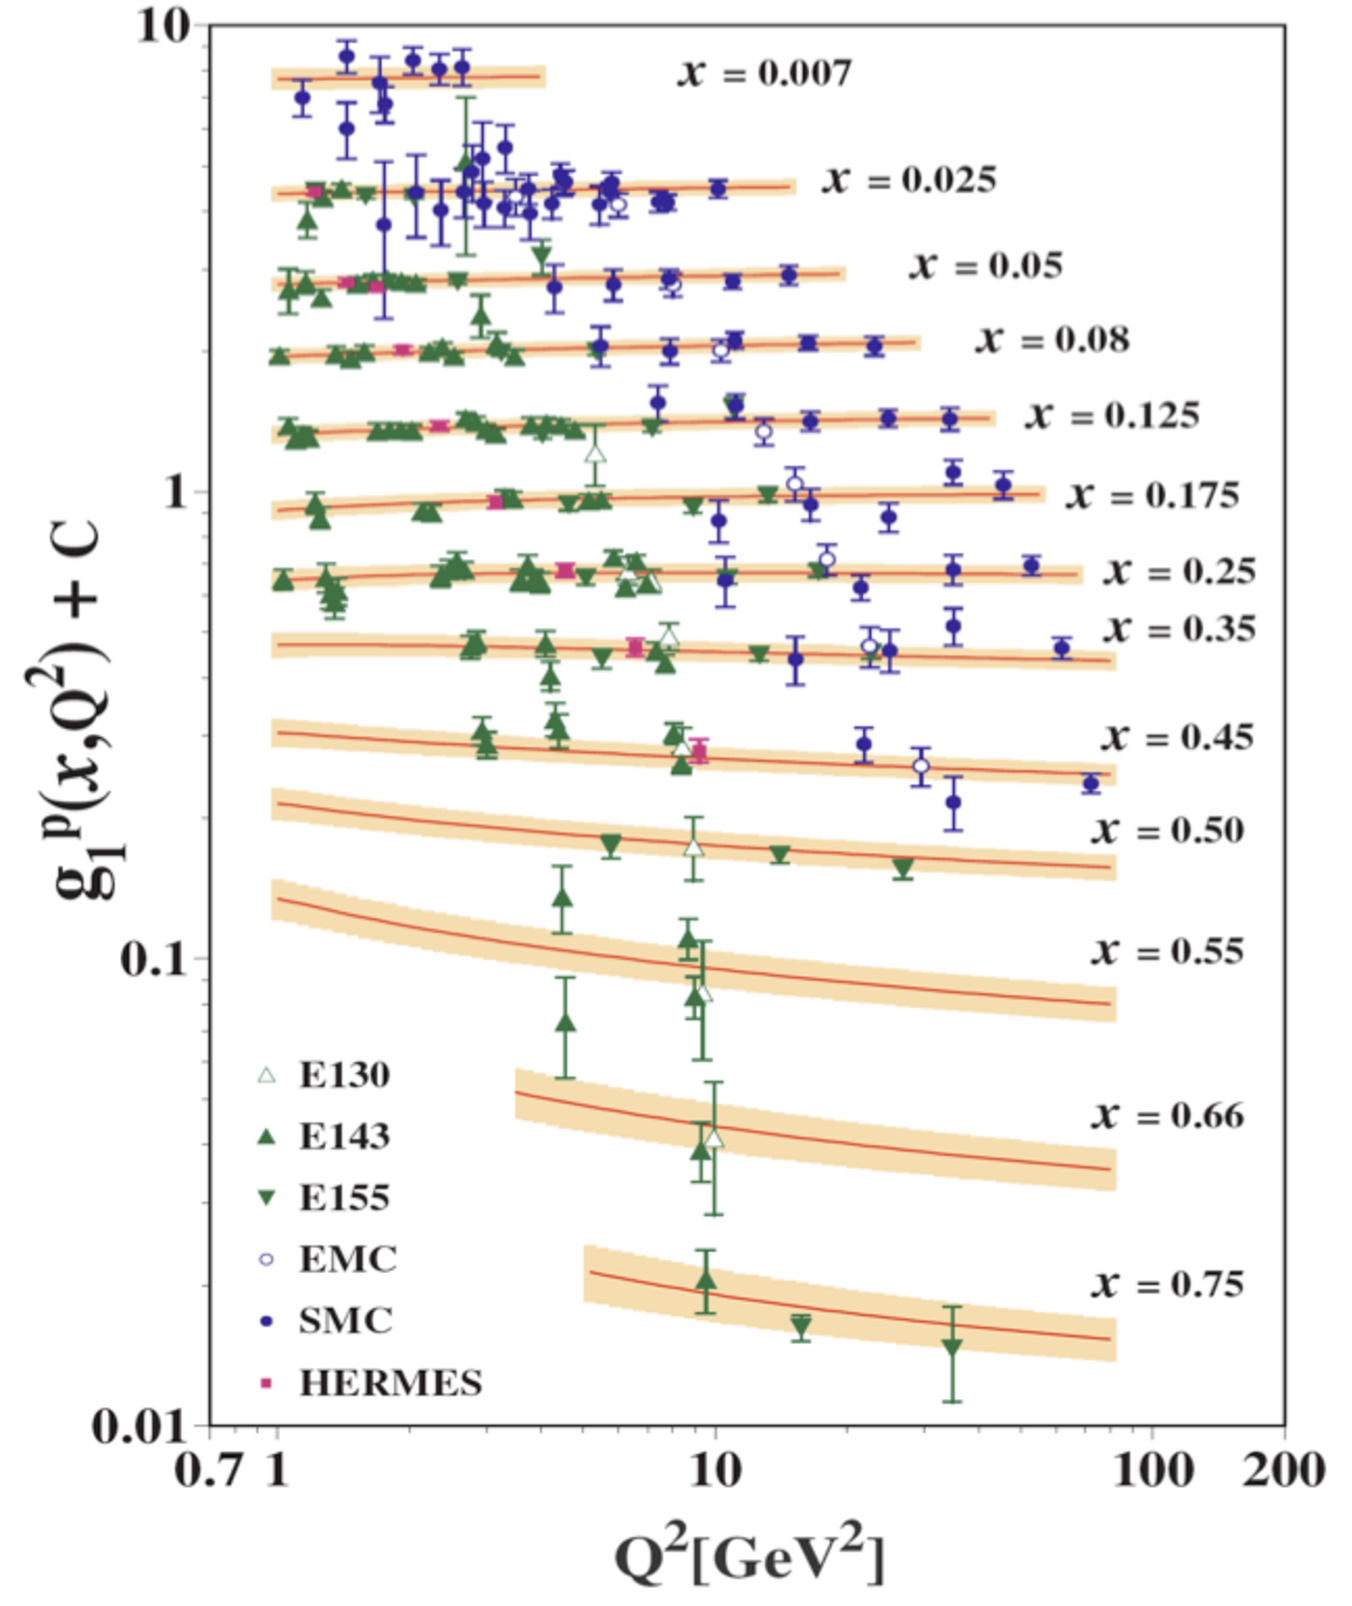
\includegraphics[width=0.7\textwidth]{figures/g1_x_q2}
  \caption{World data on the $g_1$ structure functions of the proton, plotted versus $Q^2$ for several values of $x$.  An analysis of the variation with $Q^2$ yields a parameterization of the polarization gluon distribution.} % http://www2.lns.mit.edu/eic/Bruell.pdf
  \label{fig:g1-versus-q2}
\end{figure}
% \begin{figure}
%   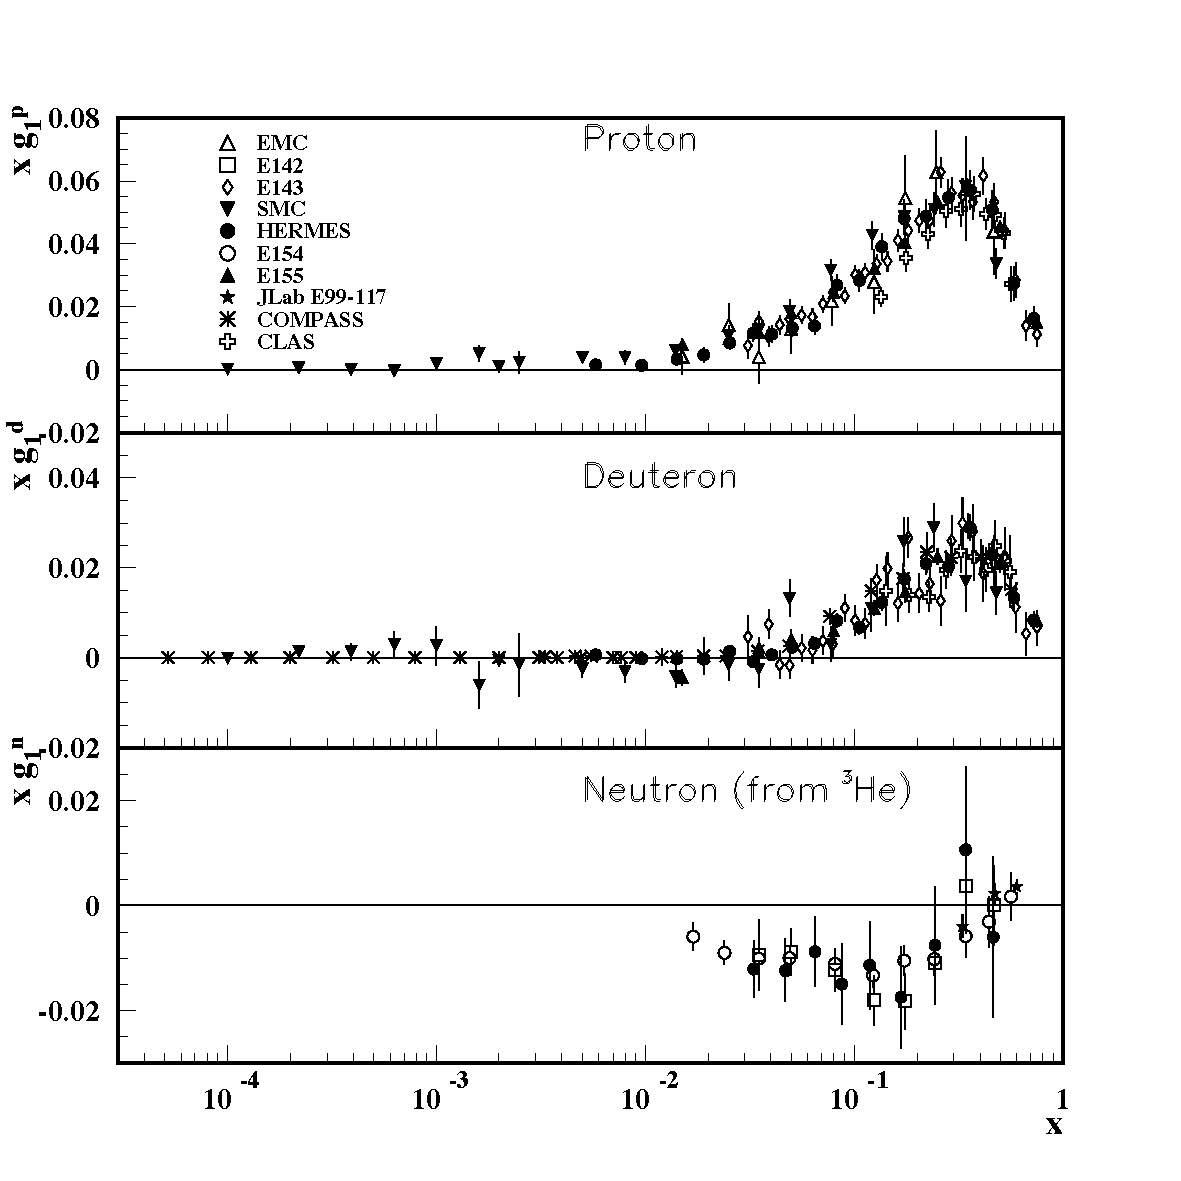
\includegraphics[width=1.0\textwidth]{figures/g1vsx}
%   \caption{World data on the $g_1$ structure functions of the proton, neutron, and deuteron \cite{Amsler:2008zzb}}
%   \label{fig:g1vsx}
% \end{figure}

% \begin{figure}
%   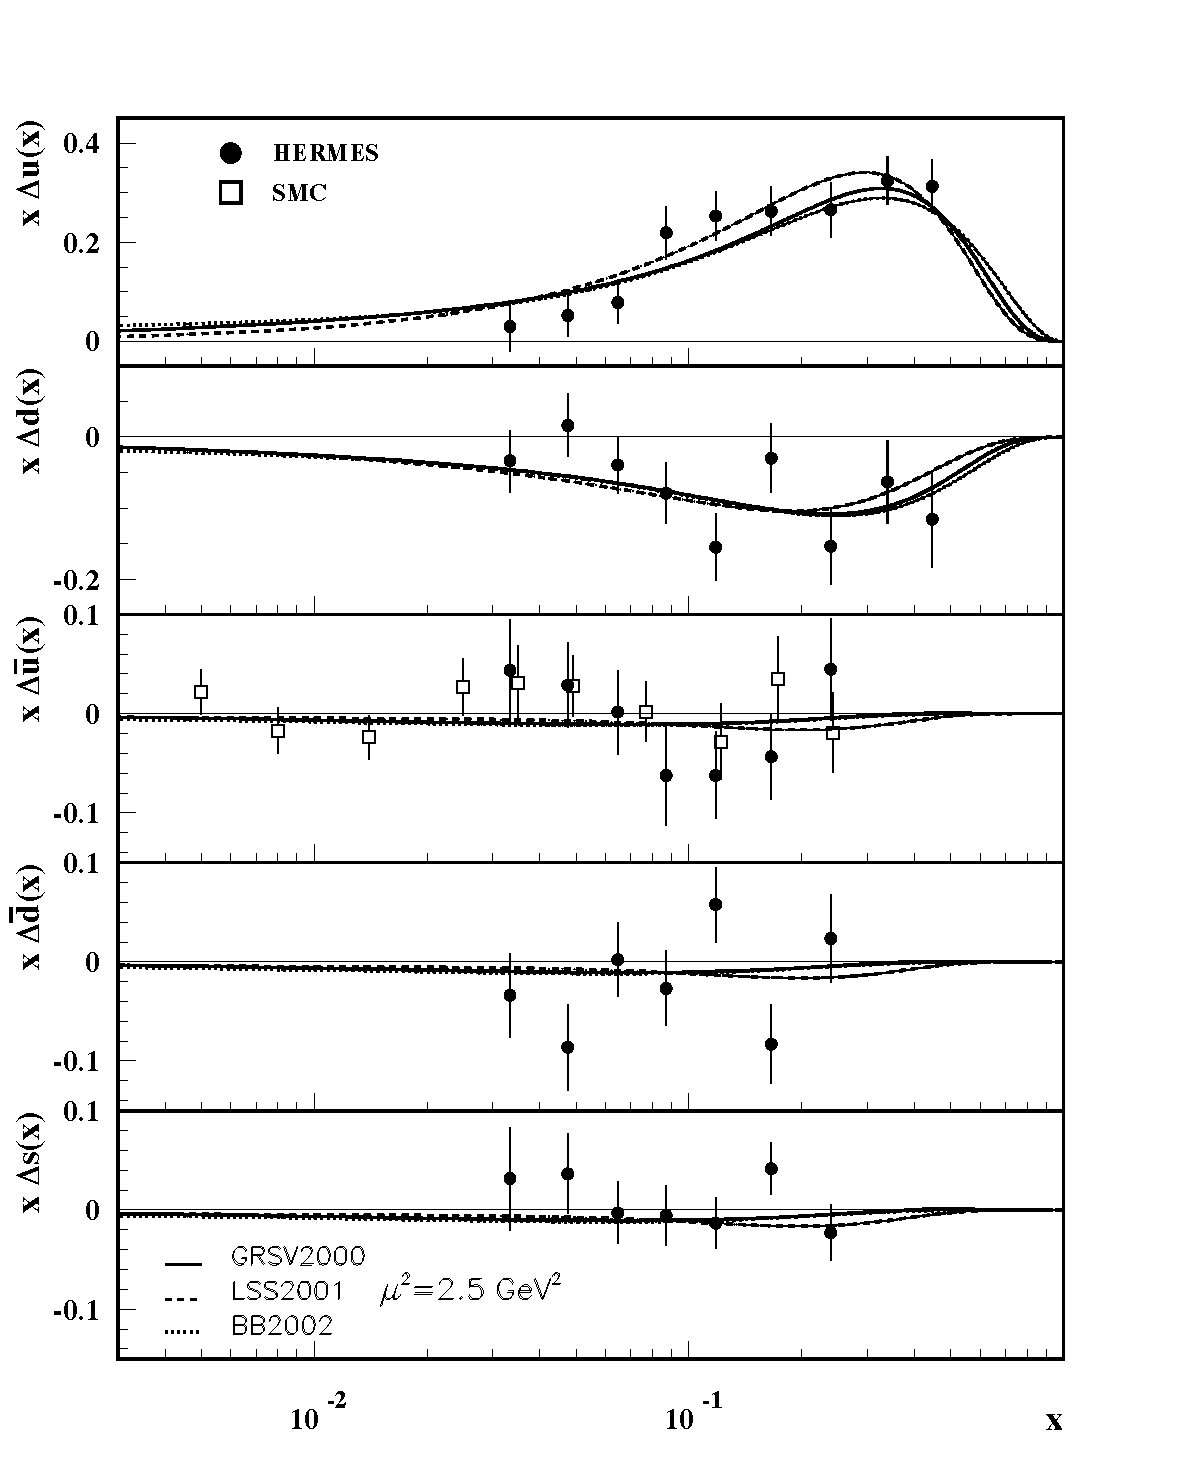
\includegraphics[width=1.0\textwidth]{figures/pol_pdf_5}
%   \caption{from the Particle Data Group \cite{Amsler:2008zzb}.  Data points are SIDIS measurements using positron (HERMES) and muon (SMC).  SMC results extracted assuming $\Delta \bar u(x) = \Delta \bar d(x)$}
%   \label{fig:pol_pdf_5}
% \end{figure}

% \begin{figure}
%   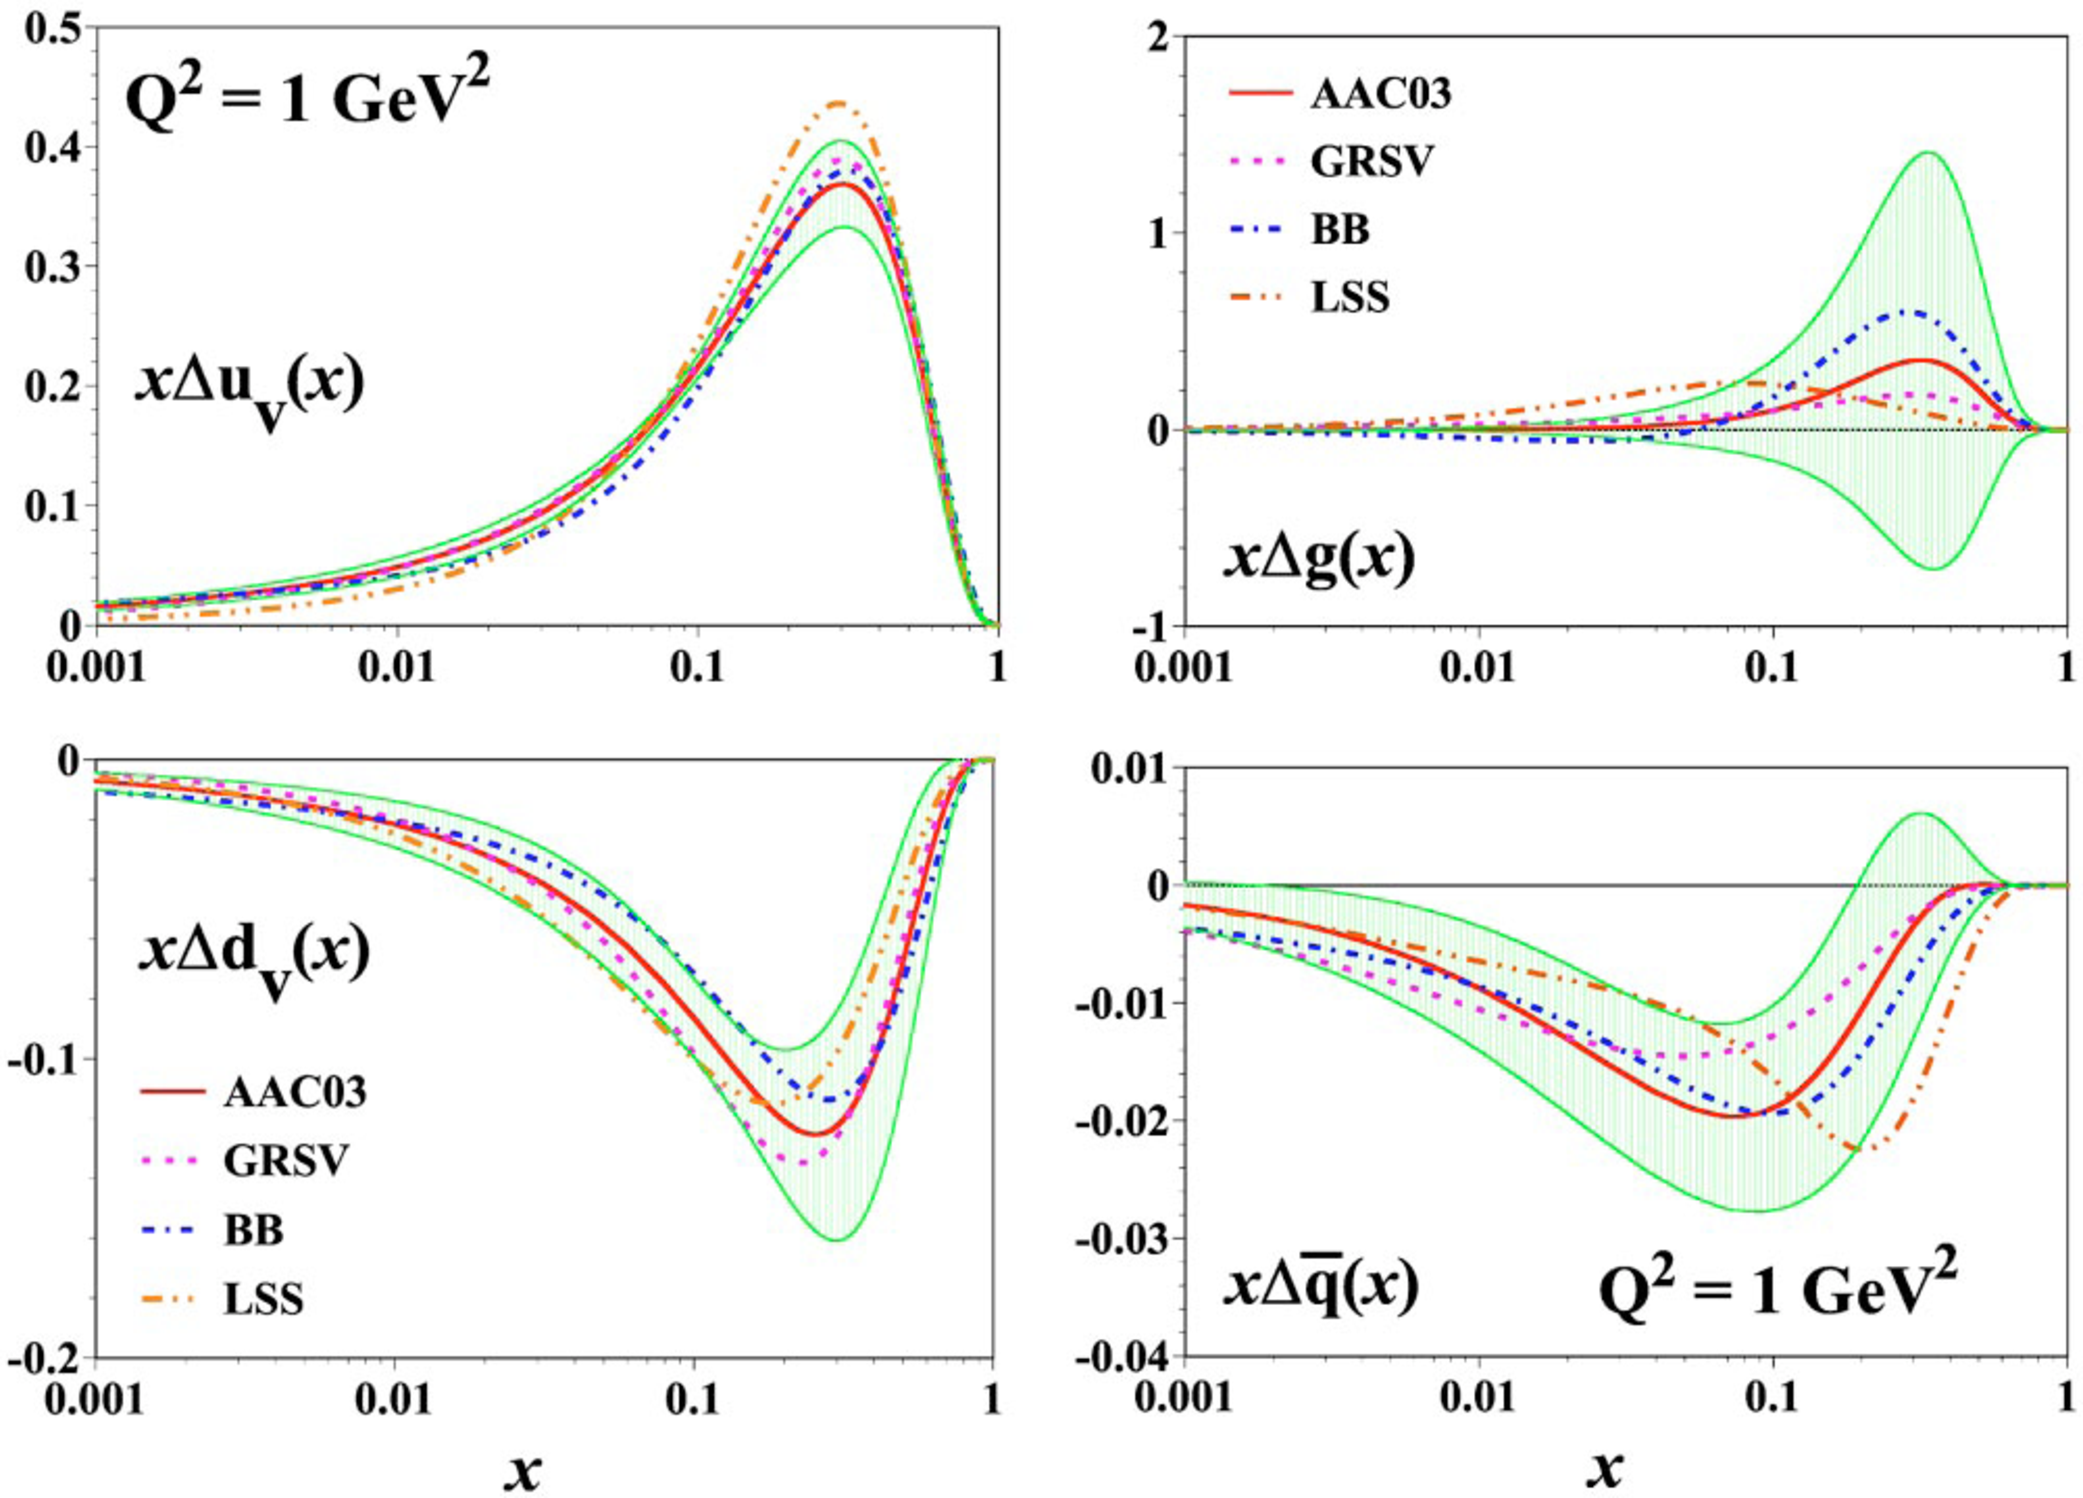
\includegraphics[width=1.0\textwidth]{figures/aac03}
%   \caption{\cite{Hirai:2003pm}  BB \cite{Bluemlein:2002be} uses ISET=3, LSS \cite{Leader:2001kh} uses $\bar{MS}$, GRSV \cite{Gluck:2000dy} uses STD.  But this is of course \textit{not} the most recent polarized PDF analysis using only DIS and SIDIS data.  My best guess at that is \cite{Leader:2006xc}}
% \end{figure}

\begin{figure}
  \centering
  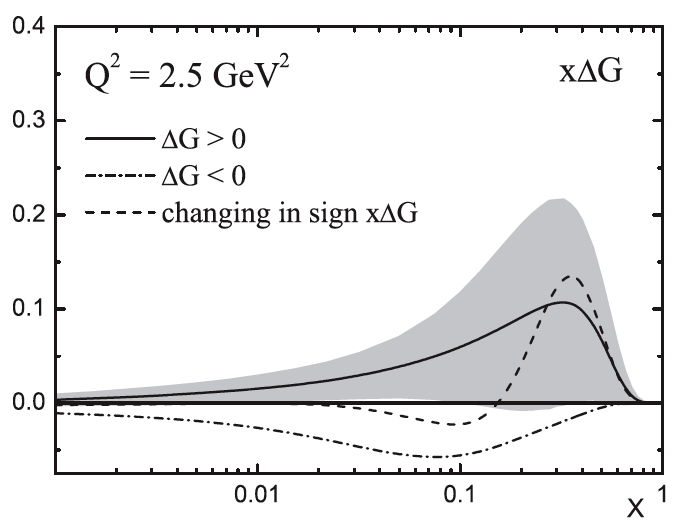
\includegraphics[width=0.6\textwidth]{figures/lss06_deltag}
  \caption{Extraction of the polarized gluon distribution from an analysis of scaling violations in DIS and SIDIS.  The gray band indicates statistical and systematic uncertainties summed in quadrature.  Analyses assuming positive, negative, and sign-changing gluon polarization all resulted in a comparable goodness-of-fit \cite{Leader:2006xc}}
\end{figure}

% Need to understand what constraints go into positive/negative/sign-changing $\Delta g(x)$ parameterizations.

\subsection{Photon-Gluon Fusion}

Given the relatively small lever arm in $Q^2$ currently available to constrain
$\Delta G$ via evolution of $g_1$, it is natural to pursue a more direct
approach involving observables that are directly linked to the gluon
polarization. In photon-gluon fusion (PGF), the lepton emits a real or virtual
photon that interacts with a gluon radiated from the nucleon to produce a
$q\bar{q}$ pair (see Figure \ref{fig:pgf}). PGF is a rare process compared to
scattering off of quarks in the nucleon, and as such analyses need a way to
enhance the signal to background ratio. The golden signature for PGF is charm
in the final state, since the nucleon itself has a negligible charm content.
Charm production has a small cross section, so analyses that look for
high-$p_T$ final states are also common.

Figure \ref{fig:pgf-deltag} summarizes results for the gluon polarization
extracted at leading order from analyses of photon-gluon fusion processes.
SMC, HERMES, and COMPASS have all released results based on the detection of
high-$p_T$ hadrons or jets, and COMPASS has released a single data point from
an analysis of charmed ($D^0$ and $D^*$) mesons. The data cover an $x$ range
of approximately $0.07 < \langle x \rangle < 0.2$ and restrict the magnitude
of the gluon polarization within that region. No NLO analysis of PGF data on
$\Delta G$ is currently available.

\begin{figure}
  \centering
  \begin{fmfgraph*}(200,150)
    \fmfleft{proton,gamma}
    \fmfright{proton',quark1,quark2}
    \fmf{fermion,width=2.5}{proton,v1}
    \fmf{fermion}{v1,proton'}
    \fmf{gluon}{v1,v2}
    \fmfblob{.15w}{v1}
    \fmf{fermion}{v2,quark1}
    \fmf{fermion}{v2,v3,quark2}
    \fmf{photon}{gamma,v3}

    % wow, it really feels like I should not have to do all of this
    \fmffixedx{0.}{v2,v3}
    \fmffixedy{0.}{v2,quark1}
    \fmffixedy{0.}{v3,quark2}
    \fmffixedy{0.}{v1,proton'}
    \fmffreeze
    \fmfshift{(0,-0.2h)}{v3}
    \fmfshift{(0.09w,-0.2h)}{quark2}
    \fmfshift{0,0.15h}{v1,proton'}
    
    % finally, add lines for outgoing quarks in struck proton
    \fmfi{plain}{vpath (__v1, __proton') shifted (thick*(-0.5,3.5))}
    \fmfi{plain}{vpath (__v1, __proton') shifted (thick*(-0.5,-3.5))}
  \end{fmfgraph*}
  \caption{Feynman diagram of photon-gluon fusion process}
  \label{fig:pgf}
\end{figure}

% this figure comes from DIS2008, but I don't see anything in SPIRES or the arXiv on it yet.  Kurek was the author
\begin{figure}
  \centering
  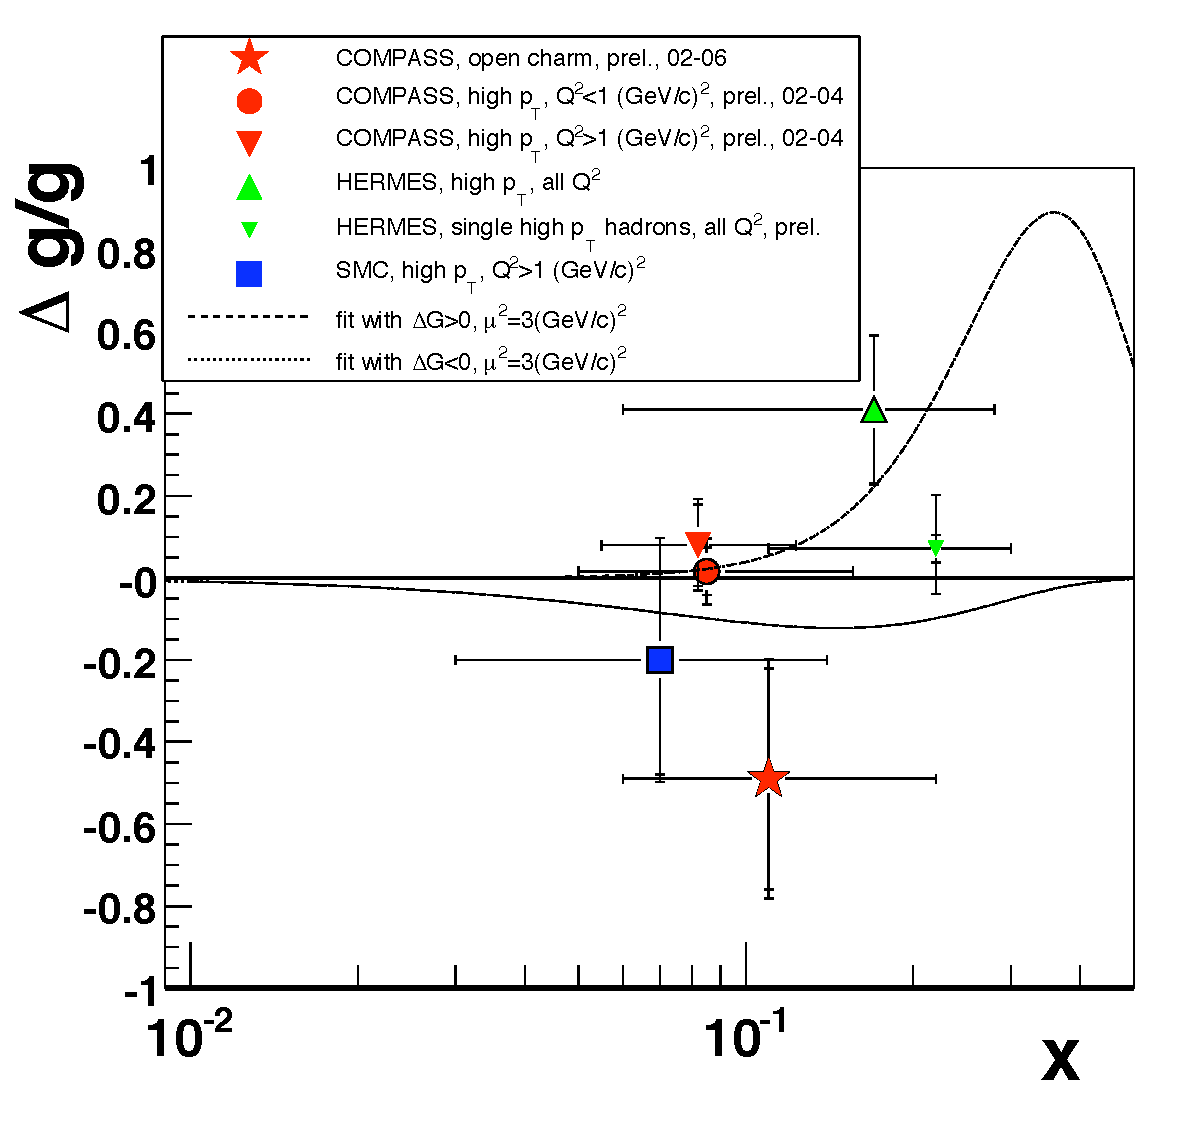
\includegraphics[width=0.7\textwidth]{figures/compass_deltag_with_prelim}
  \caption{Compilation of $\Delta g(x)/g(x)$ measurements from SMC, HERMES,
  and COMPASS plotted versus momentum fraction.}
  \label{fig:pgf-deltag}
\end{figure}

% ... this is wrong, the number is just for the COMPASS open charm measurement, the most recent LO global analysis from COMPASS yields $\Delta g(x)/g(x) = -0.49~\pm~0.27~(stat)~\pm~0.11~(syst)$ at a scale $\mu^2 \sim 13~(GeV/c)^2$ and at an average gluon momentum fraction $\langle x \rangle ~\sim 0.11$ \cite{Alekseev:2009ey}.

%% Direct \Delta G figure without preliminary results
% \begin{figure}
%   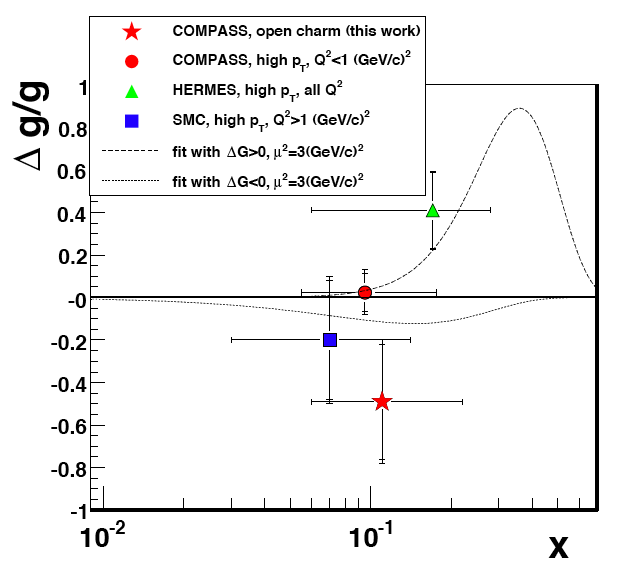
\includegraphics[width=1.0\textwidth]{figures/compass_deltag}
%   \caption{\cite{Alekseev:2009ey}}
% \end{figure}

\subsection{Lattice QCD}

Lattice QCD overestimates quark spin contribution relative to experiment
(68\%), and calculates orbital angular momentum contribution as $L_q = J_q -
\frac{1}{2}\Delta \Sigma$
\subsection{Polarized Proton Collisions}

% factorization
% universality of PDFs and FFs
% partonic cross sections calculable in perturbative QCD

The remainder of this work will focus on extracting information on $\Delta G$ from collisions of polarized proton beams, a task that is made possible by three key features of the QCD-improved parton model:

\begin{enumerate}
  \item Particle production cross sections can be factorized into a convolution of long-range parton distribution functions and fragmentation functions and a short-range partonic cross section;
  \item the parton distribution functions and fragmentation functions are universal; that is, they can be measured in one reaction and applied to any other; and
  \item partonic cross sections in the kinematic range of interest for $\Delta G$ studies are calculable using perturbative QCD.
\end{enumerate}

% The QCD-improved parton model allows us to write cross sections in factorized form as a convolution of parton distribution functions, fragmentation functions, and a parton-level cross section.
Ignoring polarization for the moment, we can express the cross section for inclusive pion production in this framework as a sum over parton flavors $i,j,k$
%
\begin{equation}
  \sigma^{pp \rightarrow \pi X} = \sum_{i,j,k} \int~dx_1 dx_2 dz~ q_i(x_1) \cdot q_j(x_2) \cdot \sigma^{ij \rightarrow k X}(x_1 p_1,x_2 p_2, p_{\pi}/z) \cdot D_k^\pi(z).
  \label{eqn:factorized}
\end{equation}
%
Here $p_1$ and $p_2$ are the momenta of the colliding proton beams and $p_{\pi}$ is the momentum of the outgoing pion, while $D_k^{\pi}(z)$ is the fragmentation function expressing the probability that a parton of flavor $k$ produces a pion carrying a fraction $z$ of the parton's momentum.\footnote{This interpretation of the fragmentation function is valid in the simple parton model, and in the QCD improved parton model if one is working in the light-cone gauge.} Equation \ref{eqn:factorized} is commonly written using the convolution notation
%
\begin{equation}
  \sigma^{pp \rightarrow \pi X} = \sum_{i,j,k} q_i \otimes q_j \otimes \sigma^{ij \rightarrow kX} \otimes D_k^\pi
\end{equation}.


\begin{equation}
  A_{LL} = \frac{\sum_{f_1,f_2,f}~\Delta f_1 \otimes \Delta f_2 \otimes \sigma^{f_1 f_2 \rightarrow f X'} \hat a_{LL}^{f_1 f_2 \rightarrow f X'} \otimes D_f}{\sum_{f_1,f_2,f}~f_1 \otimes f_2 \otimes \sigma^{f_1 f_2 \rightarrow f X'} \otimes D_f} 
\end{equation}

\begin{equation}
  \hat a_{LL}^{f_1 f_2 \rightarrow f X'} = \frac{\Delta \sigma^{f_1 f_2 \rightarrow f X'}}{\sigma^{f_1 f_2 \rightarrow f X'}}
\end{equation}

\begin{figure}\begin{center}
  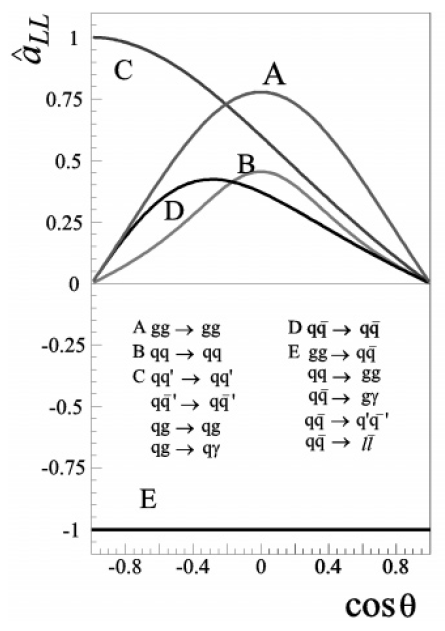
\includegraphics[width=0.5\textwidth]{figures/partonic_asymmetry}
  \caption{Lowest-order analyzing powers for various partonic subprocesses present in polarized proton collisions \cite{Bunce:2000uv}.}
\end{center}\end{figure}


%\chapter{Experimental Facilities}

\section{The Relativistic Heavy Ion Collider (RHIC)}

\begin{figure}
  \begin{center}
    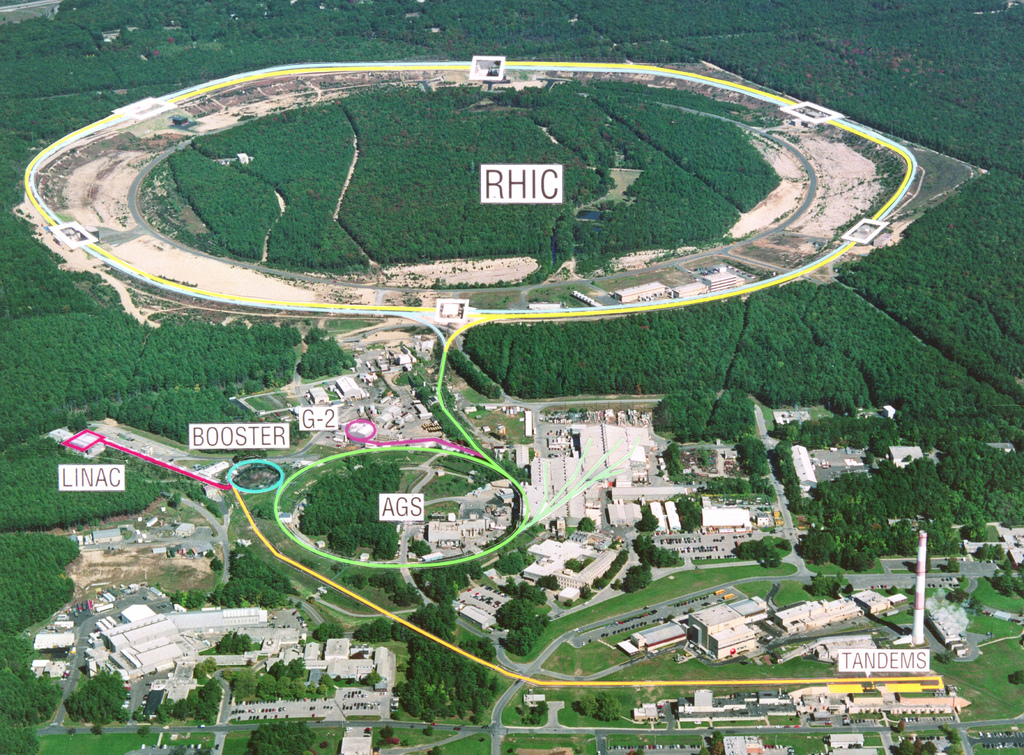
\includegraphics[width=0.8\textwidth]{figures/rhic-from-above}
  \end{center}
  \caption{The RHIC accelerator complex.  Polarized protons are generated in OPPIS (not shown) and pass through the Linac, Booster, and AGS on their way to RHIC.}
  \label{fig:rhic}
\end{figure}

The Relativistic Heavy Ion Collider (RHIC) is an intersecting storage ring located at Brookhaven National Laboratory in Upton, New York.  Unusually versatile for a collider, RHIC uses two independent superconducting rings to collide beams of ions with mass numbers separately ranging from one to 197.  Recent beam configurations include protons on protons, deuterons on gold, copper on copper, and gold on gold.  Figure \ref{fig:rhic} shows a schematic view of the RHIC accelerator complex.  The main RHIC ring has a 3.8 kilometer circumference and is comprised of six straight sections and six curved sections.  Collisions between the beams occur in the middle of each straight section; four experimental halls are situated at the two (BRAHMS), six (STAR), eight (PHENIX), and ten o'clock (PHOBOS) positions.

RHIC relies on a complex of smaller accelerators to prepare ion beams for injection into the main ring.  This work focuses on the systems used to polarize and accelerate beams of protons, thus avoiding further discussion of the Tandem Van de Graff generator used exclusively in heavy ion operations.  Polarized protons are produced using OPPIS \cite{Zelenski:2002gb, Zelenski:2008zza}, an optically-pumped polarized ion source which typically generates 0.5 mA, 400 $\mu$s pulses of ions, corresponding to $\mathrm{9x10^{11}}$ ions per pulse.  The pulsed nature of the beam is crucial to achieving the RHIC design luminosity of $\mathrm{2x10^{32}~cm^{-2}~s^{-1}}$. OPPIS polarizes protons by passing them through a rubidium vapor pumped with circularly polarized laser light in a strong magnetic field.  The $\mathrm{H^+}$ ions pick up a polarized rubidium electron through collisions in the vapor, and magnetic fields cause the electron polarization to be transferred to the nucleus.  Finally, the hydrogen atoms are ionized to $\mathrm{H^-}$ when they pass through a sodium vapor.

The pulses of 35 keV $\mathrm{H^-}$ ions produced by OPPIS are accelerated by the LINAC, Booster, and AGS on their way to RHIC.  The LINAC strips off the electrons and accelerates the protons to a kinetic energy of 200 MeV with an efficiency of approximately 50\%.  It injects the remaining $\sim \mathrm{4x10^{11}}$ ions into the Booster ring in a single bunch.  The Booster
accelerates the protons to 1.5 GeV and passes them on to the Alternating Gradient Synchrotron (AGS), which accelerates them to the RHIC injection energy of 25 GeV.  RHIC propels the $\sim \mathrm{2x10^{11}}$ protons remaining in each bunch to the desired collision energy, which can range from 30 GeV to 250 GeV.  This work analyzes data collected with a beam energy of 100 GeV.  More details of the RHIC accelerator complex are available in references \cite{Harrison:2003sb, Hahn:2003sc, Alekseev:2003sk}.

\subsection{Spin Dynamics and Siberian Snakes}

The evolution of the spin direction of a beam of polarized protons in external magnetic fields is governed by the Thomas-BMT equation \cite{Thomas:1927yu, Bargmann:1959gz},
%
\begin{equation}
  \frac{d\vec{P}}{dt} = -\left(\frac{e}{\gamma m}\right)[(G\gamma + 1) \vec{B}_{\perp} + (G + 1) \vec{B}_{\parallel}] \times \vec{P}.
\end{equation}
%
Comparing this equation with the Lorentz force equation governing the orbital motion,
%
\begin{equation}
  \frac{d\vec{v}}{dt} = -\left(\frac{e}{\gamma m}\right)[\vec{B}_{\perp}] \times \vec{v},
\end{equation}
%
one realizes that, in a pure vertical magnetic field, the spin rotates G$\gamma$ + 1 times faster than the orbital motion. This factor, referred to as the spin tune $\nu_{sp}$, gives the number of full spin precessions for every orbit.

An accelerating beam in a storage ring encounters depolarizing resonances whenever the spin tune is equal to an integer multiple of the frequency with which a spin-depolarizing magnetic field is encountered.  In the simplest case, a depolarizing field can be introduced by a magnet error or misalignment.  For these \textit{imperfection resonances}, the resonance condition is just $G\gamma = n$.  If $G\gamma$ is non-integral, the beam sees the depolarizing field at a different point in its precession on each revolution, and the effects tend to cancel out.  The focusing fields themselves can also be a source of depolarization; for these \textit{intrinsic resonances} the resonance condition is $G\gamma = kP \pm \nu_y$, where $k$ is an integer, $\nu_y$ is the vertical betatron tune, and $P$ is the superperiodicity.

The stable spin direction in an accelerating beam normally coincides with the vertical magnetic field (longitudinal polarization at the interaction points being achieved through the use of spin rotator magnets), but near a resonance it is perturbed away from the vertical by the resonance driving fields.  The polarization loss when a beam is accelerated through one of these resonances can be calculated analytically \cite{Froissart:1960zz}:
%
\begin{equation}
  \frac{P_f}{P_i} = 2 e^{-\pi |\epsilon|^2 / 2\alpha} -1.
\end{equation}
%
Here $\epsilon$ is the resonance strength and $\alpha$ is the change of the spin tune per radian of the orbit angle.  When the beam is slowly accelerated ($\alpha \ll |\epsilon|^2$) the stable spin direction changes adiabatically and the result is a spin flip.  In contrast, techniques such as a betatron tune jump effectively result in $|\epsilon|^2 \ll \alpha$ and thus preserve the polarization through the resonance.  At high energies, the number and strength of the resonances encountered make these traditional techniques impractical.  Instead, the RHIC rings employ ``Siberian Snake'' magnets \cite{Derbenev:1978hv} which generate a 180\degree spin rotation about a horizontal axis when the beam passes through them.  In effect, the Siberian Snakes ensure that the spin tune is an energy-independent half-integer, thus avoiding all imperfection resonances as well as intrinsic resonances with an appropriate choice of the betatron tune.  RHIC is designed to achieve 70\% polarization; the datasets analyzed in this work were taken with 45\% - 55\% polarized beams, as certain elements of the accelerator complex (notably, a Siberian Snake in the AGS) were still being commissioned.

\subsection{Polarimetry Systems}

RHIC polarimetry relies on the observation of small angle elastic scattering in the Coulomb-Nuclear Interference (CNI) region.  Two complementary varieties of target are used:  a thin carbon ribbon \cite{Jinnouchi:2004up} and a hydrogen gas jet (H-Jet) \cite{Zelenski:2005mz, Okada:2006dd}.  The carbon ribbon boasts a large scattering cross section which allows a statistically precise measurement of the beam polarization in a few seconds, but the theoretical prediction for the analyzing power of this measurement includes an unknown contribution from a hadronic spin flip amplitude.  In contrast, the hydrogen gas jet has a well-understood analyzing power but a much smaller scattering cross section.  The natural solution, then, is to calibrate the results of the p+C CNI polarimeters with a measurement from the H-jet polarimeter.

The p+C polarization measurements are performed using individual carbon ribbon targets in each beam that are a mere 150 $\mathrm{\mathring{A}}$ thick.  Scatterings occur at a momentum transfer of 0.002 - 0.010 $\mathrm{GeV}^2$, resulting in a small forward scattering angle for the proton and a recoil carbon nucleus with less than 1 MeV of kinetic energy.  Detection of the scattered proton is not possible without drastic changes to the beam profile at the polarimeter location, but the thinness of the target allows the recoil nucleus to escape the target and reach one of a set of silicon strip detectors arranged around it.  The use of a thin target also allows the measurement to be performed multiple times over the course of a beam store with acceptable losses in luminosity.

The theoretical uncertainty in the analyzing power of the p+C measurements is estimated to be less than 10\% \cite{Alekseev:2003sk}, but this uncertainty can be mitigated by calibrating the results from the p+C polarimeter against measurements performed using the hydrogen gas jet target.  The use of identical beam and target particles allows the polarization of the beam to be directly expressed in terms of the target polarization,
%
\begin{equation}
  P_{beam} = -P_{target}\frac{\epsilon_{beam}}{\epsilon_{target}},
\end{equation}
%
and since the target polarization is precisely measured using a Breit-Rabi polarimeter, this approach eliminates the uncertainties from the non-perturbative hadronic spin flip amplitude.  A single H-Jet polarimeter measures the polarization in both beams.  The polarimeter requires an integration time of twenty hours to achieve a 2\% statistical uncertainty for a single beam, but because the scattering cross section is so small this measurement can occur concurrently with experimental data taking.

\subsection{Cogging and Bunch Patterns}

The RHIC beams are configured into 120 RF buckets capable of storing bunches injected from the AGS.  In practice, not all of these 120 buckets are filled; a small number must be left empty as an ``abort gap'' to allow a controlled dumping of the beam when the luminosity has dropped below a useful level for physics data-taking.  The two beams are cogged so that bunches from each beam can pass through one another at the RHIC interaction points.  During a given RHIC store a given bunch from the ``Yellow'' beam always collides with the same bunch from the ``Blue'' beam.  The polarization of each bunch is independently controlled at injection time, and the mapping of polarization states to bunch numbers can vary from fill to fill, enabling a powerful control on spin-dependent systematic uncertainties at the experiments.

\section{The Solenoidal Tracker at RHIC (STAR)}

STAR \cite{Ackermann:2002ad} is a general-purpose collider detector with several subsystems capable of investigating a wide range of phenomena from multiple collision types.  A schematic of the detector is shown in Figure \ref{fig:star-schematic}.  STAR acquires data in \textit{runs}, typically of 30 to 45 minutes duration, in which several hundred thousand events will be recorded.  If a problem is discovered with a run during acquisition, reconstruction, or analysis, that run can be cleanly discarded without the loss of a large number of good events.  Four STAR subsystems are of particular interest in this work: the Beam-Beam Counters (BBCs), Barrel Electromagnetic Calorimeter (BEMC), Endcap Electromagnetic Calorimeter (EEMC), and STAR's flagship subsystem, the Time Projection Chamber (TPC).  The BBCs and BEMC identify interesting events online and trigger the detector to read them out, while the BEMC, EEMC and TPC are used to reconstruct the final state of the event offline.  The BBCs also allow a bunch crossing-dependent measure of the beam luminosities, which is essential to normalize spin-dependent asymmetries.  These and other subsystems are described in greater detail in \cite{RHIC-Special-Issue}.

\begin{figure}
  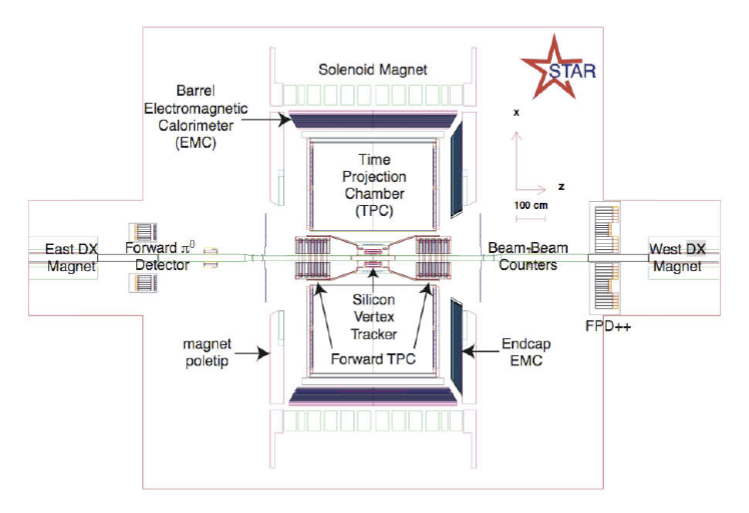
\includegraphics[width=1.0\textwidth]{figures/star-schematic}
  \caption{Schematic overview of the STAR detector, identifying many of the detector subsystems and defining the STAR coordinate system.}
  \label{fig:star-schematic}
\end{figure}

\subsection{Trigger System}

STAR has a 3 level hardware trigger system (L0, L2, L3) \cite{Bieser:2002ah, Adler:2002ab} allowing for the selection of rare events from the large pool of minimum bias (MB) interactions.   While the TPC and other tracking detectors have long readout times compared to the interaction rate, the BBCs and the BEMC are fast detectors that sample each bunch crossing at the STAR IR, and can thus be used for efficient selection of high $p_T$ events.  A typical trigger mix consists of $\sim$10-20 separate triggers running in parallel.  Significant improvements to the STAR data acquisition system (DAQ) beyond design specifications have increased the rate of event recording to typical values of 30-50 Hz, with a dead-time fraction of $\sim$50\%.

The L0 trigger operates on coarse-granularity data from fast detectors and builds a decision tree capable of completing its analysis in time with the 119 nanosecond RHIC bunch crossing interval.  If the L0 trigger issues an accept the full trigger detector data is sent to L2 for further analysis.  In contrast to L0, the L2 trigger runs on commodity hardware and its algorithms can be written in C.  It applies preliminary calibrations and can do some primitive jet finding in the course of making its decision, but must issue that decision in no more than 5 milliseconds.  If the L2 trigger issues an accept, the slow detectors are read out and the full event is recorded to tape.  The L3 trigger \cite{Adler:2002ab} enables online TPC track finding using a farm of commodity servers.  It was at one time a necessary component of the trigger system, but upgrades to the data acquisition system have increased the throughput from STAR to the RHIC Computing Facility (RCF) to the point where the $\sim$50 Hz of events selected by the L0 and L2 trigger algorithms can be recorded to tape.  The L3 tracking output continues to serve as a useful qualitative monitoring tool in the STAR control room.

\subsection{Beam Beam Counters}

The BBCs \cite{Kiryluk:2005gg} are segmented scintillator annuli situated $\pm$ 3.5 meters along the beam line from the center of STAR.  They are sensitive to charged particles in the pseudorapidity range $3.3 < |\eta| < 5.0$, where pseudorapidity is defined in terms of the angle between the particle momentum and the beam momentum as $\eta \equiv -\mathrm{ln}\left(\mathrm{tan} \frac{\theta}{2}\right)$.  Coincident signals in both BBCs define the minimum-bias (MB) trigger condition for proton-proton collisions at STAR; most trigger algorithms use the MB condition as a base on which to apply more selective criteria.

In addition to defining the MB trigger condition, coincident signals in the BBCs can also serve as a luminosity monitor.  In particular, tracking the number of BBCs coincidences per bunch crossing allows one to measure the luminosities for each combination of the spin states of the two beams.  The ratios of these luminosities are a crucial element in the extraction of single- and double-spin physics asymmetries at RHIC.

\subsection{Electromagnetic Calorimeters}

Electromagnetic calorimetry is an essential element of the trigger system at STAR and is also important for many final state analyses (especially, for the purposes of this thesis, jet reconstruction).  We will focus on two calorimeter subsystems: the BEMC \cite{Beddo:2002zx}, covering $|\eta| < 1.0$, and the EEMC \cite{Allgower:2002zy}, which is installed only on the West side of STAR and spans $1.09 < \eta < 2.0$.  Both the BEMC and EEMC are segmented sampling calorimeters with lead absorber layers and active plastic scintillator layers.  The BEMC is divided into 4800 projective towers spanning $\Delta \eta \times \Delta \phi = 0.05 \times 0.05$, while the EEMC's 720 projective towers each span 0.1 in azimuth and range in pseudorapidity coverage from $\Delta \eta = 0.057$ at $\eta = 1.09$ to $\Delta \eta = 0.099$ at $\eta = 2.0$.  Both calorimeters have a depth of at least twenty radiation lengths.%  Table \ref{table:emc-comp} summarizes the design characteristics of the two subsystems.

At Level 0, the BEMC and EEMC implement trigger conditions based on thresholds in single high towers, 4x4 (4x2) trigger patches, and 20x20 (12x10) jet patches.  At Level 2 the calorimeters drive a wide variety of trigger algorithms ranging from dijet reconstructions that span seamlessly across the two calorimeters to heavy flavor searches doing online calculations of tower pair invariant masses.  The primary calorimeter trigger condition used in this work is the BEMC jet patch (JP) trigger, which requires an energy sum above threshold in one of twelve fixed collections of 400 towers each spanning $\Delta \eta \times \Delta \phi = 1.0 \times 1.0$.  In this case the Level 2 trigger algorithm is a simple accept, and the EEMC is used only for final state jet reconstruction.

%% This table is probably not a good idea anyway.
% \begin{table}
%   \begin{center}
%     \begin{tabular}{c|cc}
%       & BEMC & EEMC\\
%       \hline
%       depth & $\geq 20~\chi_0$ & $\geq 20~\chi_0$
%     \end{tabular}
%   \end{center}
%   \caption{PID Selection Windows}
%   \label{tbl:pid-selection-windows}
% \end{table}

\subsection{Time Projection Chamber}

The TPC \cite{Anderson:2003ur} is the primary detector subsystem at STAR, providing full azimuthal tracking of charged particles with transverse momentum above $\sim 100$ MeV/c and $|\eta| < 1.8$, and particle identification through measurements of ionization energy loss.  It is a 4.2 meter long volume of gas bounded by an inner field cage at a radius of 50 centimeters and an outer field cage at 200 centimeters.  The end caps of the detector are held at ground potential and the central cathode membrane at -28kV; metal rings connected by precision resistors in the field cages ensure a uniform electric field of $\approx 135$ V/cm.  The TPC sits inside a solenoid with a field strength of 0.5 Tesla.

Charged particles ionize the P10 gas as they traverse the volume of the TPC, producing secondary electrons that drift to the nearest end cap of the detector.  The $z$ coordinate of each point along the track is calculated by measuring the time required for the electrons to reach the end cap and dividing by the drift velocity.  The drift velocity varies with electric field strength and with the temperature, pressure, and composition of the gas, so measurements of it are performed every few hours using the TPC laser system \cite{Abele:2003aa}.  Radial laser beams at known positions along the length of the TPC ionize trace organic substances in the P10 gas; the time difference between the arrival of electrons liberated by lasers at two different positions allows a calculation of the drift velocity.

% could say a little more about how electron drift time is measured ... e.g. time buckets for readout pads
Each end cap is divided into twelve sectors, positioned as the hours on a clock face, and each sector contains 45 rows of cathode pads (5,692 pads per sector).  The cathode pads are mounted on anode wires; the secondary electrons avalanche near the anode wires, and the positive ions produced in this avalanche generate a temporary image charge on several nearby pads.  The image charge is measured, and an analysis of the charge sharing between the pads allows the original track $x$ and $y$ coordinates along the wire to be reconstructed to within a small fraction of a pad width.  Finally, the charge deposited on each pad is used to calculate the particle's energy loss per unit length due to ionization, or dE/dx.

\begin{figure}
  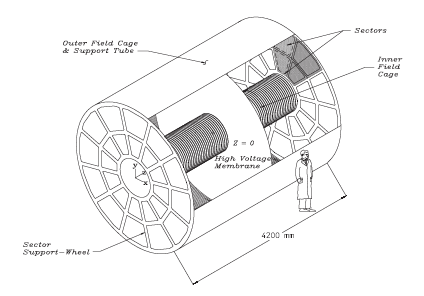
\includegraphics[width=1.0\textwidth]{figures/tpc}
  \caption{The STAR Time Projection Chamber (TPC).  The end-caps are divided into twelve sectors, each with an inner and outer sub-sector.  The TPC is divided into two by a central cathode membrane spanning the gas volume between the inner and outer field cages.}
  \label{fig:tpc}
\end{figure}

\subsection{Computing Facilities}

The aggregate raw data produced by all detector subsystems in STAR is on the order of 100 MB per event.  The STAR Data Acquisition System (DAQ) \cite{Landgraf:2002zw} reduces the event size through hardware-based zero suppression, resulting in a 10x savings for the highest multiplicity heavy ion collisions and substantially greater savings (100x or more) for the proton-proton collisions analyzed in this work.  It then organizes the data into DAQ files and transfers these files to tape in the RHIC Computing Facility's HPSS hierarchical storage system, which provides 8 PB of storage and a throughput of over 300 MB per second to the RHIC and USATLAS experiments.

Event reconstruction and data analysis takes place on a Linux compute farm with over 3300 cores and 1.7 PB of local storage.  The STAR reconstruction software  is written in C++ and runs on Scientific Linux, a version of Red Hat Enterprise Linux maintained by the particle physics community.  The event reconstruction code loads DAQ files from HPSS into local storage, performs tracking and applies a variety of detector calibrations, and generates ``micro Data Storage Tapes'' or ``$\mu$DSTs'', which contain higher-level physics objects such as particle tracks, event vertices, and calorimeter clusters.  $\mu$DSTs are implemented using ROOT \cite{Brun:1997pa} TTrees, allowing efficient ad-hoc and batch data analysis.  The analysis presented here was performed on a set of TTrees generated from $\mu$DSTs using a mix of custom C++ libraries and Python scripts interfacing with the ROOT data analysis framework.

%\chapter{Event Reconstruction}
\section{Detector Response Simulations}

An accurate simulation of the detector response is an important validation of a collaboration's understanding of the apparatus as well as a vital tool in the calculation of some systematic uncertainties. STAR, like many other collider experiments, uses Monte Carlo routines to generate events with properties similar to those measured by the experiment.  These events are collections of identified particles with well-defined kinematics.  STAR primarily relies on the PYTHIA 6 event generator \cite{Sjostrand:2006za} in the CDF Tune A \cite{Field:2005sa} configuration to simulate proton collisions.  A subset of results from PYTHIA have been validated using the alternative HERWIG event generator \cite{Corcella:2000bw}.  The output from PYTHIA is fed through a GEANT 3.21 \cite{GEANT321} model of the STAR detector; the end results of this process is a set of detector signals that approximate the actual detector response to a real event.  Significantly, the output from GEANT can be processed by the same reconstruction software used for real data.  Reconstruction efficiencies and other quantities useful for the estimation of systematic uncertainties can calculated by associating particles in the output of the reconstruction software with particles in the ``true'' event record generated by PYTHIA.

\section{Triggering and Data Acquisition}

The basic building block of nearly all physics analyses in the 200 GeV pp program is the minimum-bias (MB) trigger defined by coincident signals in the East and West BBCs, yielding a sensitivity of 26.1$\pm$2.0 mb (87\%) of the NSD cross section as deduced from a Vernier scan performed in 2003. On top of the MB trigger STAR layers a variety of requirements based on signals in the electromagnetic calorimeters that bias the event sample towards rare events with large transverse energy depositions.

The dominant trigger algorithm in this analysis is the BEMC jet patch (JP) trigger, which sums transverse energy depositions over fixed groups of 400 towers covering an area of $\Delta \eta \times \Delta \phi$ = 1.0 $\times$ 1.0.  The JP trigger is designed for efficient, minimally-biased selection of high-energy jets.  The threshold for the primary JP trigger in the 2005(2006) run was 6.4(8.3) GeV, and the trigger sampled an integrated luminosity during longitudinal running of 3.3(9.3) $pb^{-1}$.

% The 8.3 number excludes transverse running.  Including that the 06 number would be 1.95 (1st long) + 3.20 (trans) + 6.30 (2nd long) = 11.45
% also assumes a MB cross section of 25 mb, not 26.1 as stated here
% http://www.star.bnl.gov/protected/common/common2006/trigger2006/lum_pertriggerid_pp2006.txt

% 2006 DSM prescales
% mysql --host=dbbak.starp.bnl.gov --port=3405 Conditions_rts
% SELECT run.idx_rn, dict.value FROM dict,run WHERE dict.hash=run.dicthash AND dict.label='mb-prescale' AND run.idx_rn<7160000 AND dict.value>0;

% Regular prescales, event counts (port 3404 for 05, port 3405 for 06)
% mysql --host=dbbak.starp.bnl.gov --port=3405 RunLog
% SELECT run, offlineTriggerID, prescale, numberOfEvents FROM l0TriggerSet;

% my thresholds assume final calibrations, I think

% Jamie's integrated lumi numbers are somewhat smaller than mine, presumably because of some basic quality cuts.  My numbers for 06 BJP1 are

% 117221 2.4
% 127221 3.6
% 137221 0.1
% 137222 6.8

% for a total sampled lumi from longitudinal running of 9.3, rather than 8.3

\section{Tracking}
\section{Spin Sorting}

Each of the bunches in the two RHIC beams is polarized independently, and the
polarization pattern can change from fill to fill. An accurate record of the
spin state of each bunch crossing in a fill is essential for any spin
analysis. The polarization pattern for the rings is set by the RHIC
Collider-Accelerator Department (C-AD) and broadcast through the CDEV
\cite{Barton:2003sh} control and monitoring system. The pattern is formatted
as a list of 360 8 bit numbers, one for each of the time buckets in RHIC, and
is defined in terms of the bunch crossings at the 12 o'clock position in the
RHIC ring. The beam experiences an odd number of spin flips in between 12
o'clock and the STAR IP at six o'clock, so the beam polarizations at STAR are
flipped relative to the broadcast record. The interpretation of each bit is
given in Table \ref{tbl:spin8}.

\begin{table}
  \begin{center}
  % \begin{ruledtabular}
    \begin{tabular}{c|l}
      \hline
      bit & meaning \\
      \hline
      \hline
      0 & yellow beam filled\\
      \hline
      1 & yellow beam polarized up\\
      \hline
      2 & yellow beam polarized down\\
      \hline
      3 & yellow beam unpolarized\\
      \hline
      4 & blue beam filled\\
      \hline
      5 & blue beam polarized up\\
      \hline
      6 & blue beam polarized down\\
      \hline
      7 & blue beam unpolarized\\
      \hline
    \end{tabular}
  % \end{ruledtabular}
  \end{center}
  \caption{Significance of each of the bits in an eight bit spin record.}
  \label{tbl:spin8}
\end{table}

A given bunch from the Blue ring always collides with the same bunch from the
Yellow ring at a specific interaction point in the RHIC ring over the course
of a fill. C-AD has historically configured the beams so that bunch zero from
the Blue beam collides with bunch zero from the Yellow beam at the PHENIX IP,
and as a result the PHENIX experiment sees only one abort gap in its fill
patterns. The situation is different at STAR, where the RHIC ``toggle mode''
defines the pairs of bunches from the Blue and Yellow beams that collide. The
toggle mode is typically set once at the beginning of the RHIC data-taking
period, and is encoded implicitly in the spin patterns broadcast by CDEV.

After accounting for the spin flip and the toggle mode, an analysis must map
the event IDs recorded at the experiment to the 7 bit bunch crossing IDs
defined by CDEV in order to determine the spin state of a given event. The
STAR Trigger receives this information from RHIC for every event, but analyses
have observed occasional inaccuracies in the feed that render it unreliable.
Instead, STAR uses a more robust 48 bit counter synchronized to the 9.4 MHz
RHIC clock to uniquely identify every event. The 7 bit bunch crossing IDs can
be expressed in terms of this 48 bit counter as
%
\begin{equation}
  \mathrm{7~bit~ID} = \left(\mathrm{48~bit~counter} + \mathrm{offset}\right)~mod~120
\end{equation}
%
The offset is calculated for each STAR run by generating 120 histograms of
triggers versus the 7 bit bunch IDs for each possible value of the offset,
comparing these histograms to a histogram of the intended spin pattern at
STAR, and searching for a minimum in the $\chi^2$ distribution. An example of
the overlap between the trigger rate versus bunch crossing ID and the spin
pattern after the correct offset has been applied is shown in Figure
\ref{fig:bxing-offset}. The offsets for each STAR run are calculated once and
uploaded to the STAR Calibrations DB which allows them to be applied by all
STAR spin analyses. Further details of the spin state determination can be
found in Reference \cite{spin-db-website}.

\begin{figure}
  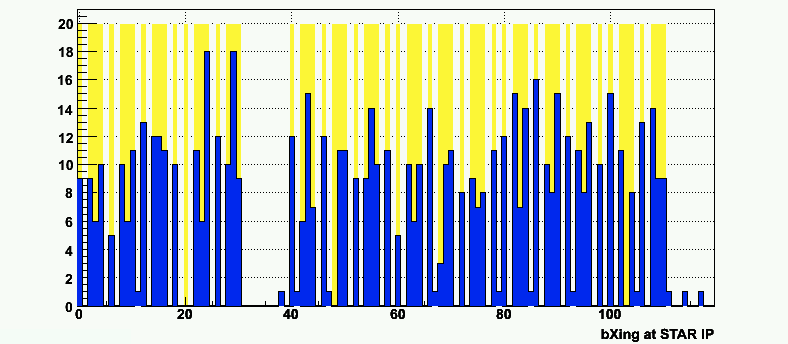
\includegraphics[width=1.0\textwidth]{figures/bxing-offset-determined}
  \caption{Distribution of events (blue) versus the corrected 7 bit bunch
  crossing IDs at the STAR interaction point. The yellow bars indicate the
  bunch crossings where both beams have filled bunches according to the
  intended spin patterns broadcast by CDEV.}
  \label{fig:bxing-offset}
\end{figure}

\section{Jet Finding}

\subsection{Clustering Algorithm}

STAR has implemented the midpoint-cone algorithm in accordance with the
recommendations of Reference \cite{Blazey:2000qt}. The algorithm proceeds by
assembling a $p_{T}$ ordered list of four momenta (``protojets") for each
event. Each protojet with $p_T>p_{T}^{seed}$ (``seeds") initiates a clustering
sequence. For each clustering sequence, protojets within an angular distance
$\Delta r = \sqrt{\Delta\phi^{2} + \Delta\eta ^{2}} < r_{cone}$ are selected
and their four momenta are added to define the four momentum of the cluster
via $p_{\mu}^{cluster} = \sum p_{\mu}^{i}$. If $p_{\mu}^{cluster}$ lies within
a distance $\epsilon$ of the initiating protojet, the clustering sequence
terminates. Otherwise the clustering sequence is iterated about the direction
$p_{\mu}^{cluster}$ until convergence is reached. Once stable configurations
are identified, the association is cataloged for later use. However, no
protojets are removed from the sample. Clustering continues until the list of
seeds is exhausted, yielding a list of redundant, overlapping, stable
clusters. Before disentangling the stable clusters, the algorithm first tests
for missed initiating directions by constructing a set of test seed directions
at the ``midpoint" between all possible pairs of neighboring clusters.
Specifically, locations at the midpoint of all cluster pairs separated by
distance $d < 2 \times r_{cone}$ are tested for stable cluster configurations.
Clusters formed around midpoint seeds are only retained if the resulting
cluster lies within $\epsilon$ of the midpoint seed, and no iteration is
performed.

After all midpoint seeds have been tested, the resulting list of stable
clusters is disentangled via a splitting/merging algorithm. The algorithm
proceeds by finding the highest $p_{T}$ cluster, referred to as the ``root"
cluster. Next, all clusters sharing protojets with the root cluster
("neighbors") are identified, and the neighbor with the largest $p_T$ is
selected. The root and neighbor jet are merged if
$\frac{p_{T}^{shared}}{p_{T}^{neighbor}}>f_{split-merge}$ where $0 <
f_{split-merge} < 1$. If this condition is not satisfied the clusters are
split such that each protojet is assigned to the closest of the two
overlapping clusters. After each split/merge, the cluster list is again sorted
by $p_T$, a new root cluster is chosen, and the splitting/merging continues
until no protojets are shared amongst clusters. It is important to note that
the split/merge step takes a list of clusters that are essentially circular,
while the final clusters are no longer necessarily circular. Finally, each of
the unique clusters is tagged as a ``jet", whose four momentum is the vector
sum of the constituent protojets.

\subsection{Application at STAR}

STAR applies the midpoint-cone algorithm to cluster charged particle tracks
and BEMC tower energies as follows. Charged particle protojets are constructed
from all primary TPC tracks satisfying the aforementioned cuts. A charged pion
mass is assumed when relating energy and momentum. Each BEMC tower energy
measurement is corrected for charged particle energy deposition by i)
identifying the number of TPC tracks projecting to the tower and ii)
subtracting the most probable MIP energy deposition for each of the projecting
tracks. After MIP subtraction, each tower energy measurement is converted to a
four momentum using knowledge of the highest-ranking primary vertex location
and assuming a photon mass. Protojets are then constructed for towers with
corrected $E_{T}>0.2 $GeV.

The midpoint-cone algorithm first sorts the protojets onto a grid of
$\Delta\eta=\Delta\phi=0.05$, where the properties of each grid ``cell" are
defined by the vector sum of its constituent protojets. This discretization
improves computational efficiency and minimizes potential biases arising from
the fact that the BEMC towers may measure energy from more than one particle.
Each cell maintains a list of its constituent protojets so that there is no
ultimate loss of information. The midpoint cone algorithm then operates on the
list of cells, and after clustering and splitting/merging conclude, each
cluster is then characterized by the vector sum of its constituent four
momenta. Jets with $p_{T}<5$ GeV/$c$ are discarded. The control parameters of
the clustering algorithm are listed in Table \ref{tbl:jetfinding-parameters}.
The restricted cone radius in the 2005 analysis was motivated by the limited
pseudorapidity acceptance of the partially installed BEMC.

\begin{table}
  \begin{center}
    % \begin{ruledtabular}
      \begin{tabular}{c|c|c}
      Parameter & Value & Explanation\\
      \hline \hline
      $r_{cone}$  &   0.4 (2005), 0.7 (2006) & clustering radius \\ \hline
      $p_{T}^{seed}$  &   0.5 GeV/$c$ & seed threshold \\ \hline
      $f_{split-merge}$  &  0.5  & split/merge criterion \\ \hline
      $\epsilon$  &  0.025  & clustering convergence condition \\
      \end{tabular}
    % \end{ruledtabular}    
  \end{center}
  \caption{Control parameters used in midpoint-cone clustering.}
  \label{tbl:jetfinding-parameters}
\end{table}

\section{Charged Pion Identification}

Charged pions are identified and separated from kaons, protons, and electrons by the amount of energy they lose in the TPC.  The dE/dx of a TPC track is obtained by sorting the track hits according to energy loss, removing the top 30\%, and averaging the rest.  Track dE/dx values for a given particle species at a fixed momentum are Gaussian, so one can also express the dE/dx value for each track in terms of a deviation from the mean dE/dx for some identified particle at that track's momentum.  In particular, track energy loss values at STAR are commonly given in terms of ``$n\sigma(\pi)$'', the deviation from the mean of the pion peak divided by the width of said peak.  Protons and kaons fall to the left of the pion peak (lower energy loss) and electrons fall to the right (higher energy loss).

The peak position of the raw $n\sigma(\pi)$ distribution generated by the STAR reconstruction software exhibits some significant time dependence, so instead of assuming a fixed mean of 0.0 for the pion Gaussian,  this analysis performs a triple Gaussian fit on the $n\sigma(\pi)$ distribution for each fill and extracts time-dependent means to better calibrate the PID cut.  After this recalibration one can extract yields for the various species of charged particles by fitting the $n\sigma(\pi)$ distributions with a multi-Gaussian parametric function.  The fitting procedure starts with 8 Gaussians -- one each for $\pi^{+}$, $\pi^{-}$, $K^{+}$, $K^{-}$, $p$, $\bar{p}$, $e^{+}$, and $e^{-}$.  The number of free parameters is reduced by applying the following constraints:

\begin{itemize}
    \item all widths must be equal (dE/dx resolution isn't particle-dependent)
    \item particle/antiparticle pairs should have the same mean
    \item $\pi - K$, $\pi - p$, and $\pi - e$ separations are known from other analyses \cite{Xu:2008th}
\end{itemize}

In the end there are 24 - 7 - 4 - 3 = 10 free parameters in the fit:  the Gaussian width, the position of the $\pi$ Gaussian, and the yields.  The particle separations change as a function of momentum, not $p_{T}$, so we slice a $p_{T}$ bin into momentum bins and fit each one individually.  Figure \ref{fig:typical-nsigmapi} shows a typical fit result.  The tracks have been shifted by 6*charge in order to plot positive and negatively charged tracks on the same histogram.

\begin{figure}
  \begin{center}
    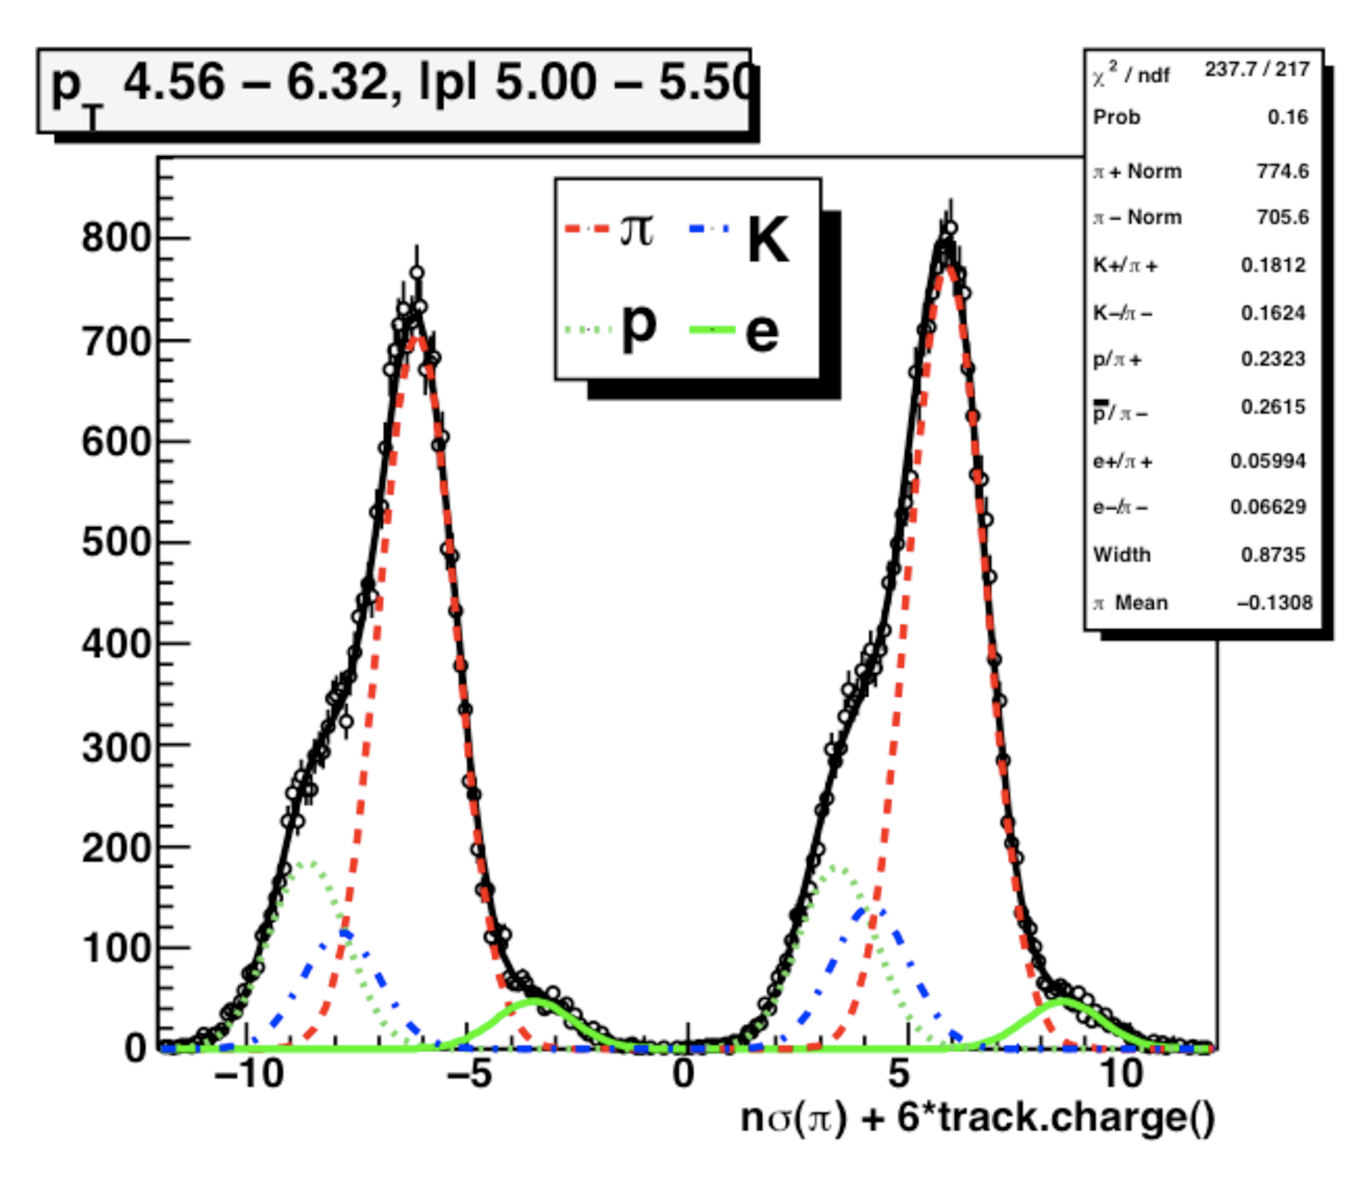
\includegraphics[width=0.7\textwidth]{figures/typical-nsigmapi}    
  \end{center}
  \caption{Example PID fit result}
  \label{fig:typical-nsigmapi}
\end{figure}

With this database of particle yields in hand we can calculate the set of PID cuts that minimize the statistical uncertainty on the background-subtracted $A_{LL}$ (Equation \ref{eqn:sigma-all}).  A simple minimization routine assuming $\sigma_{A_{LL}}^{2} = 1/N$ for the raw asymmetries yields the results in Table \ref{tbl:pid-selection-windows}.

\begin{table}
    \begin{center}
        \begin{tabular}{c|ccc}
        \hline
        $p_{T}$ bin & $\pi$ window & proton/kaon max & electron min\\
        \hline
        \hline
        [2.00 - 3.18] & (-1.10, 2.30) & -2.10 & 2.60\\
        \hline
        [3.18 - 4.56] & (-1.40, 2.10) & -2.10 & 2.40\\
        \hline
        [4.56 - 6.32] & (-1.40, 1.80) & -2.10 & 2.40\\
        \hline
        [6.32 - 8.80] & (-1.40, 1.80) & -2.10 & 2.40\\
        \hline
        [8.80 - 12.84] & (-1.30, 1.40) & -2.10 & 2.10\\
    \hline
    \end{tabular}
    \end{center}
    \caption{PID Selection Windows}
    \label{tbl:pid-selection-windows}
\end{table}



%\chapter{Analysis}

\section{$A_{LL}$ Methodology}

Let's start with the equation for a raw double spin asymmetry:

\begin{equation}
  A_{LL} = \frac{\sum_{runs} P_{Y}P_{B}(N_{++} - RN_{+-})}{\sum_{runs} P_{Y}^{2}P_{B}^{2}(N_{++} + RN_{+-})}
\end{equation}
%
where R is a ratio of spin-dependent luminosities determined from the BBC scaler system:

\begin{equation}
  R = \frac{\mathcal{L}_{UU}+\mathcal{L}_{DD}}{\mathcal{L}_{DU}+\mathcal{L}_{UD}}
\end{equation}
%
Each of the $\mathcal{L}_{ij}$ is a sum of the scaler counts from board 5 for
timebins 7, 8, and 9 for events with a given spin state (in terms of 4 bit
spin states, UU = 5, DU = 6, UD = 9, and DD = 10). The formula for the
statistical uncertainty on $A_{LL}$ neglects uncertainties on the relative
luminosities and beam polarizations. Assuming Poisson statistics on $N_{++}$
and $N_{+-}$ we have for a single run

\begin{equation}
  \left(\frac{\sigma_{A_{LL}}}{A_{LL}}\right)^2 = \frac{N_{++} + R^2 N_{+-}}{(N_{++} - R N_{+-})^2} + \frac{N_{++} + R^2 N_{+-}}{(N_{++} + R N_{+-})^2} - 2\frac{N_{++} + R^2 N_{+-}}{N_{++}^2 - R^2 N_{+-}^2} \times COV(N_{++} - R N_{+-}, N_{++} + R N_{+-})
\end{equation}
%
where the covariance term is just

\begin{equation}
  COV(N_{++} - R N_{+-},~N_{++} + R N_{+-}) = N_{++} - R^2 N_{+-}
\end{equation}
%
In the case of small asymmetries, the relative uncertainty on the numerator
dominates the uncertainty on $A_{LL}$:

\begin{eqnarray}
  \left(\frac{\sigma_{A_{LL}}}{A_{LL}}\right)^2 & = & \left(N_{++} + R^2 N_{+-}\right) \left[\frac{1}{(N_{++} - R N_{+-})^2} + \frac{1}{(N_{++} + R N_{+-})^2} - \frac{2(N_{++}-R^2 N_{+-})}{N_{++}^2 - R^2 N_{+-}^2} \right] \\
  & \approx & \frac{N_{++} + R^2 N_{+-}}{(N_{++} - R N_{+-})^2}
\end{eqnarray}
%
ROOT's TH1::Divide method does the error propagation correctly in this limit
(it ignores the covariance), so we rely on it to calculate the results. The
generalization to a sum over runs is straightforward since the yields for each
run are uncorrelated.

\subsection{Multi-Particle Statistics}

In this analysis it's very often the case that we accept multiple pions from a
single event. Treating each of these particles as an independent event and
simply using $\sqrt{N}$ for the errors as we did in the previous section is
not quite correct. Following the prescription in
\href{http://www.star.bnl.gov/protected/spin/sowinski/analysis/derivations/multiParticle.pdf}{Jim's
note on multi-particle statistics} we fill each bin in a histogram at most
once per event, using a weight equal to the number of particles that fell into
that bin. Note that this approach does not account for correlations across
bins.

\subsection{Background Subtraction}

Next we consider asymmetries with sideband subtraction. Specifically, the raw
charged pion asymmetries in this analysis are contaminated by protons, kaons,
and electrons. The protons and kaons are necessarily combined into a single
sideband. Both sidebands have some non-negligible pion contribution. We start
by defining a reduced background fraction that accounts for the impurities in
the sideband:

\begin{equation}
  f_{x}(y) = \frac{x~counts~in~y~window}{total~in~y~window}
\end{equation}

\begin{equation}
  f'(x) = \frac{f_{x}(\pi)}{1 - f_{\pi}(x)}
\end{equation}
%
The standard equations for the background-subtracted $A_{LL}^{\pi}$ and its
statistical uncertainty are only modified by replacing the background fraction
for each sideband with its reduced background fraction:

\begin{equation}
  A_{LL}^{\pi} = \frac{ A_{LL}^{\pi,raw} - f'(p+K)A_{LL}^{p+K,raw} - f'(e)A_{LL}^{e,raw} }{1 - f'(p+K) - f'(e) }
  \label{eqn:all}
\end{equation}

\begin{equation}
  \sigma_{A_{LL}^{\pi}} = \frac{\sqrt{ \sigma_{A_{LL}^{raw}}^{2} + f'(p+K)^{2} * \sigma_{A_{LL}^{p+K,raw}}^{2} + f'(e)^{2} * \sigma_{A_{LL}^{e,raw}}^{2} }}{1 - f'(p+K) - f'(e)}
  \label{eqn:sigma-all}
\end{equation}


\section{Beam Polarizations}

\subsection{Polarization Vectors and Transverse Asymmetries}
\section{Luminosity Determination}

Our statistical uncertainties on $A_{LL}$ assume perfect knowledge of the
relative luminosity of the different spin states. This systematic addresses
that simplification.

\subsection{Uncertainty Evaluation Using the ZDCs}

% \textit{Note: \href{http://mare.tamu.edu/star/2005n06Jets/2005relLumSys_mar29_2008/}{analysis by Murad Sarsour}}

We can quantify the precision with which we understand the relative luminosities
obtained from the BBCs by using an independent luminosity monitor, the ZDCs. In
the absence of non-statistical fluctuations, the uncertainty on R will be
dominated by the statistics in the ZDCs, which count at a much lower rate than
the BBCs during proton-proton running.

A couple of problems in the ZDC data need to be corrected before a comparison
to the BBCs can be trusted. The first problem is due to the ``killer bit''
algorithm, which suppressed signals in the ZDCs for 10 bunch crossings after
an initial signal. The algorithm is used in heavy ion running to prevent
ringing in the calorimeters from generating false signals, but in pp running
it biases the ZDC counts. Bunch crossings immediately following abort gaps
(where the killer bit is more likely to be off) end up with more ZDC counts
than crossings in the middle of a filled set of bunches. As a result, the
ratio of relative luminosities obtained from the ZDC and BBC will not be flat,
see Figure \ref{fig:zdctobbc6170012zoom}.

\begin{figure}
  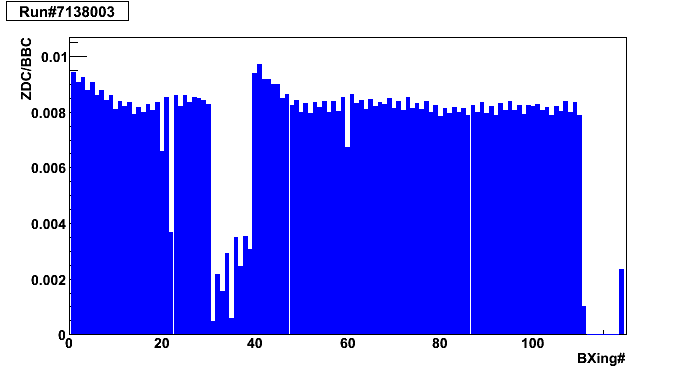
\includegraphics[width=1.0\textwidth]{figures/ZDCtoBBC_r7138003}
  \caption{Ratio of ZDC and BBC counts versus bunch crossing.  Notice that the ratio is larger in bunch crossings immediately following abort gaps.}
  \label{fig:zdctobbc6170012zoom}
\end{figure}

The procedure developed to correct for this effect requires scaling the counts
for a given bunch crossing by a factor that takes into account the frequency
with which the previous ten bunch crossings had a signal. For the ZDC singles
rates, the formula for the corrected counts $n_{j}$ in a given bunch crossing
$j$ is
%
\begin{equation}
  n_{j}^{corrected} = n_{j} * \frac{N_{cycles}}{N_{cycles} - \sum_{i=1}^{10}n_{j-i}}
\end{equation}
%
where $N_{cycles}$ is the number of times the beam cycled through STAR in the
run. Figure \ref{fig:zdc-singles-ratio} shows the effect of applying the
correction for a sample run.

\begin{figure}
  \subfloat{
    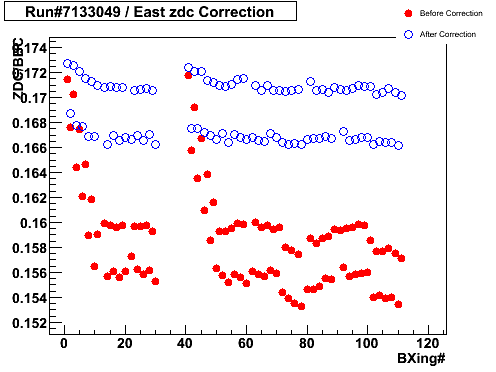
\includegraphics[width=0.5\textwidth]{figures/ZDCtoBBC_r7133049ER}
  }
  \subfloat{
    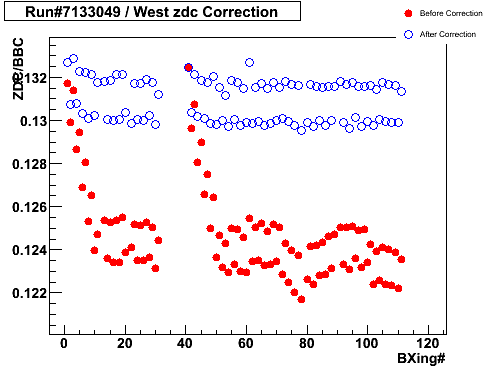
\includegraphics[width=0.5\textwidth]{figures/ZDCtoBBC_r7133049WR}
  }
  \caption{Change in the ZDC singles rates after applying the killer bit correction.}
  \label{fig:zdc-singles-ratio}
\end{figure}

The formula to correct the ZDC coincidence counts is complicated by the need
to track the killer bits for the two detectors simultaneously. The formula for
the corrected coincidence counts $c_{j}$ given singles counts $e_{j}$ (ZCDE)
and $w_{j}$ (ZDCW) is
%
\begin{align}
  &\alpha_{j} = N_{cycles} - \sum_{i=1}^{10}c_{j-i} \notag\\
  &\beta_{j} = \sum_{i=1}^{10}(e_{j} + w_{j} - 2*c_{j}) - \sum_{i=1}^{9}\left[\frac{(e_{j}-c_{j}) * (w_{j}-c_{j})}{\alpha_{j}-(e_{j-10}-c_{j-10})} + \frac{(e_{j}-c_{j}) * (w_{j}-c_{j})}{\alpha_{j}-(w_{j-10}-c_{j-10})}\right] + ... \notag\\
  &c_{j}^{corrected} = c_{j} * \frac{N_{cycles}}{\alpha_{j} - \beta_{j}} 
\end{align}
%
and the effect of the killer bit correction on the coincidence distributions
is shown in Figure \ref{fig:coinRat6143016}

\begin{figure}
  \begin{center}
    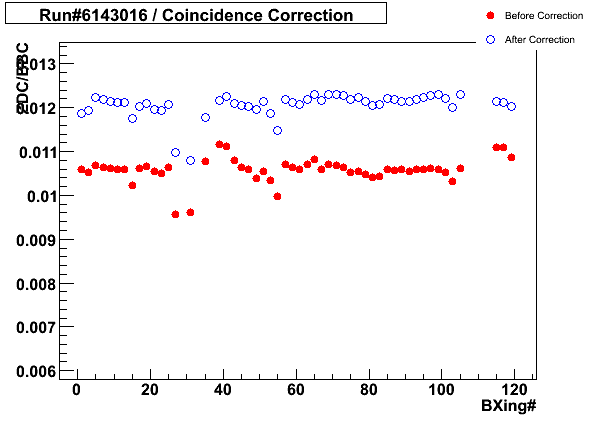
\includegraphics[width=0.6\textwidth]{figures/coinRat6143016}
  \end{center}
  \caption{Change in the ZDC coincidence rates after applying the killer bit
  correction.}
  \label{fig:coinRat6143016}
\end{figure}

\begin{figure}
  \begin{center}
    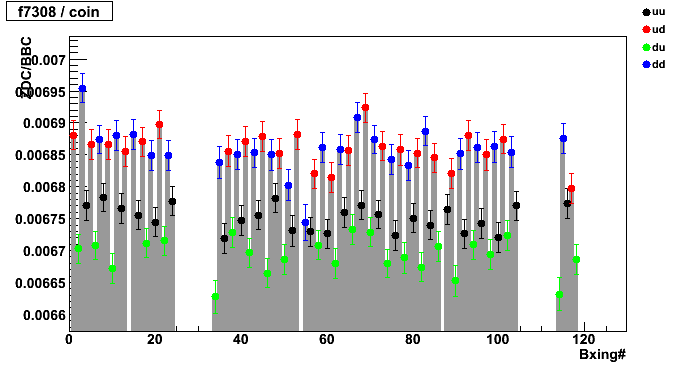
\includegraphics[width=0.8\textwidth]{figures/c7308}
  \end{center}
  \caption{Example of a coherent spin pattern and even-odd ZDC rate
  oscillation. In this case, the ZDC rate is always higher when the spin of
  the blue beam is down.}
  \label{fig:c7308}
\end{figure}

The second problem that we need to correct has come to be known as the
``even-odd'' effect. It turns out that the ZDC coincidence rates are often
different for even-numbered and odd-numbered bunch crossings. This oscillation
can introduce a false asymmetry if it aligns coherently with a particular spin
pattern. For instance, in Figure \ref{fig:c7308} we see that the ZDC
coincidence rates are always higher when the spin of the blue beam is down.
Figure \ref{fig:fevfod} shows the time dependence of this even-odd
oscillation, with the colors now representing individual fills. To quantify
the bias this introduces on $A_{LL}$, we can define the fractional overlap
between the even-odd ZDC oscillation and relevant portion of the spin pattern
for $A_{LL}$ using a 120 element vector $|EO\rangle = |+1,-1,+1,-1,...\rangle$
and another 120 element vector $|LL\rangle$ whose elements are 1 if the bunch
crossing is UU or DD, -1 if UD or DU, and 0 otherwise. The inner product of
these vectors measures the susceptibility of $A_{LL}$ for that spin pattern to
any even-odd oscillation.

\begin{figure}
  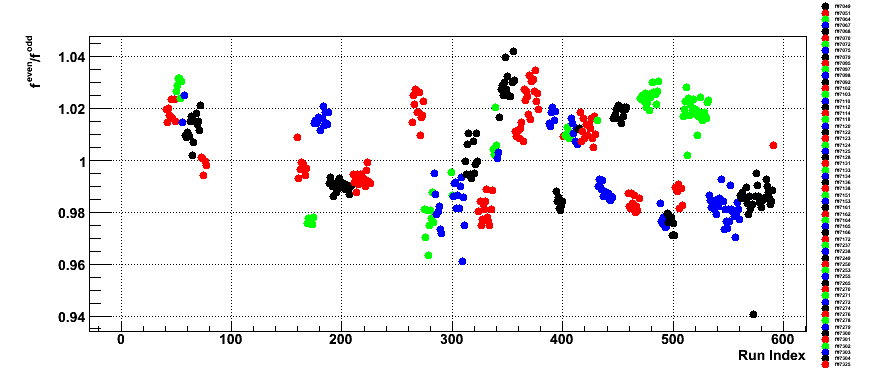
\includegraphics[width=1.0\textwidth]{figures/fevfod}
  \caption{Magnitude of even-odd rate asymmetry versus time.}
  \label{fig:fevfod}
\end{figure}

It turns out that $A_{LL}$ is less biased by the even-odd rate oscillation in
the ZDC than, say, the blue beam single-spin asymmetry. Figure \ref{fig:cll}
plots the fill-by-fill change in $A_{LL}$ if the ZDC is used for relative
luminosities instead of the BBC against the the product of the fractional
overlap $F \equiv \langle EO | LL \rangle$ and the magnitude of the even-odd
oscillation $S-1$. Placing a cut on $|F*(S-1)| < 0.002$ is well-motivated. For
fills without reliable ZDC information, we use Figure \ref{fig:fevfod} to
assume a conservative $|S-1| = 0.03$.

\begin{figure}
  \begin{center}
  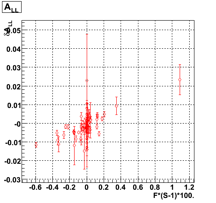
\includegraphics[]{figures/cll}
  \end{center}
  \caption{Change in $A_{LL}$ versus the product of the even-odd rate oscillation amplitude and the fractional overlap $\langle EO | LL \rangle$.  Deviations from 0 on the x-axis indicate fills where $A_{LL}$ is biased by the even-odd effect.}
  \label{fig:cll}
\end{figure}

After correcting for the killer bits and rejecting the fills that fail the
even-odd oscillation cut the uncertainty on $A_{LL}$ due to the uncertainty in
the relative luminosities is estimated to be $9.32\times10^{-4}$.

\subsection{Beam Background Bias}

\textit{Note: \href{http://www.star.bnl.gov/protected/spin/kowalik/2005/r-lumi/bkg_sys.html}{analysis by Kasia Kowalik}}

The relative luminosities obtained from the BBCs might also be biased by false
signals generated by beam-gas background. We can try to quantify this by
studying the coincidence rate in crossings where one of the two beams has an
unfilled bunch (``abort gaps''). The beam-gas background is assumed to be
crossing- and spin-independent, but it can be different in each beam. It
follows that the per-crossing coincidence rate due to beam-gas in each beam is
just the average number of BBC coincidences found in the abort gaps for that
beam. In Figure \ref{fig:bkg-yellow-blue}, the x-axis is the background rate
divided by the total rate, defined as the average number of coincidences per
bunch crossing with a spin state of UU, UD, DU, or DD. The two histograms are
incremented for each STAR run. We see that the background rate in the BBCs due
to beam-gas is typically less than 0.1\% of the total rate.

\begin{figure}
  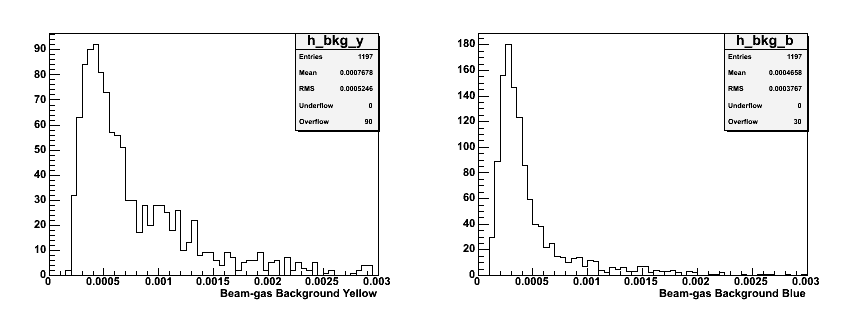
\includegraphics[width=1.0\textwidth]{figures/bkg-yellow-blue}
  \caption{Fraction of the total coincidence rate attributed to beam gas in
  each beam. The histograms are incremented once for each STAR run.}
  \label{fig:bkg-yellow-blue}
\end{figure}

Given run-dependent background fractions for both beams, it's possible to
calculate background-subtracted relative luminosities. Figure
\ref{fig:r-lumi-sys-bkg} shows the difference between the raw relative
luminosity and the background-subtracted version. The background-corrected
relative luminosities yield an $A_{LL}$ that differs from the original by
$3.0\times10^{-4}$, so we use that as the uncertainty for this source of
systematic error.

\begin{figure}
  \begin{center}
    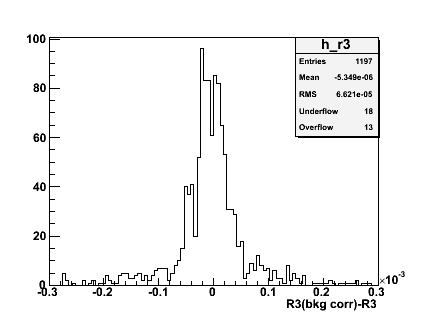
\includegraphics[width=0.6\textwidth]{figures/r-lumi-sys-bkg}
  \end{center}
  \caption{Change in the relative luminosities after correcting for beam-gas
  background.}
  \label{fig:r-lumi-sys-bkg}
\end{figure}


\section{Trigger and Reconstruction Bias}

We determine the size of this systematic uncertainty using a leading-order Monte Carlo evaluation of $A_{LL}$.  We start with the kinematics and hard scattering subprocess of each Pythia event and determine numerator and denominator weights by calculating a partonic $a_{LL}$ and sampling from polarized and unpolarized parton distribution functions.  We can use these weights to calculate an $A_{LL}$ for any set of simulated events.  Specifically, we can measure the difference between the ``true'' $A_{LL}$ for all Pythia events and the ``reconstructed'' $A_{LL}$ using only triggered events with reconstructed charged pions and use that to assign the systematic uncertainty.

This procedure obviously requires that our Monte Carlo generator does a good job of reproducing the actual event kinematics.  Unfortunately, we have found that the fragmentation tune in Pythia 6.4 is not quite up to the task.  In Figure \ref{fig:subprocess-fractions} we compare the subprocess contributions to charged pion production reported by Pythia with the results of NLO pQCD calculations incorporating Kretzer and DSS fragmentation functions.  The DSS set is known to better describe RHIC kinematics, but in Figure \ref{fig:subprocess-fractions} it's clear that Pythia agrees much better with Kretzer.  

\begin{figure}
  \subfigure[Kretzer]{
    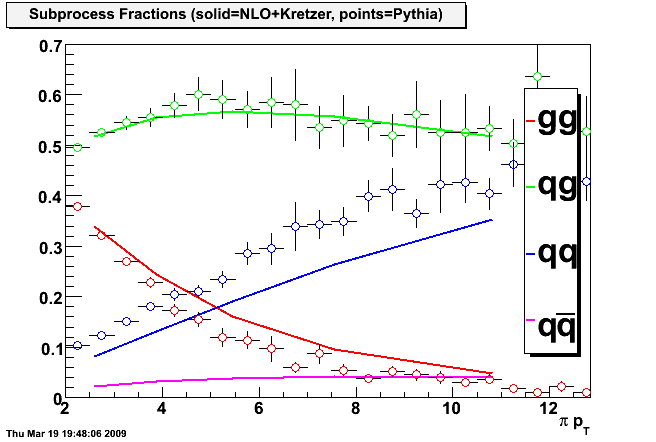
\includegraphics[width=0.5\textwidth]{figures/pythia-kretzer}
    \label{fig:pythia-kretzer}
  }
  \subfigure[DSS]{
    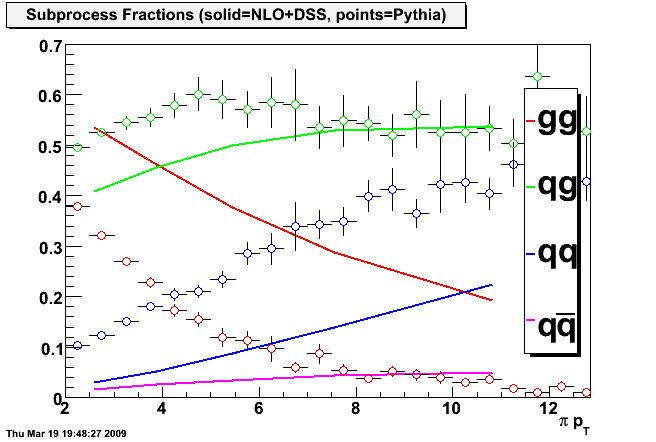
\includegraphics[width=0.5\textwidth]{figures/pythia-dss}
    \label{fig:pythia-dss}
  }
  \caption{Comparison of subprocess contributions to charged pion production
  in Pythia and NLO pQCD calculations incorporating two different
  fragmentation functions. The Pythia results agree much better with the
  calculations using Kretzer fragmentation functions}
  \label{fig:subprocess-fractions}
\end{figure}

Getting the subprocess contributions right is an important precondition for using the Method of Asymmetry Weights to evaluate trigger and reconstruction bias, quite simply because $A_{LL}$ has such a strong subprocess dependence.  To confirm that the problem is really isolated to Pythia's fragmentation functions, we examined the ratio of pions fragmenting from the quark and the gluon in qg scattering events.  That ratio is shown in Figure \ref{fig:qg-fragmentation}, and confirms that the fragmentation model is Kretzer-like, with much softer gluon fragmentation and/or harder quark fragmentation than we observe at RHIC.

\begin{figure}
  \begin{center}
    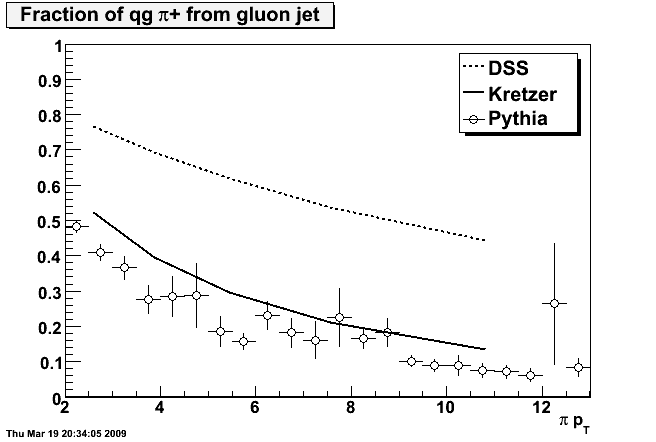
\includegraphics[width=0.7\textwidth]{figures/qg-fragmentation}
  \end{center}
  \caption{Fraction of pions produced in quark-gluon scattering events that
  fragment from the gluon. Once again, the Pythia distributions agree much
  better with the calculation that uses Kretzer fragmentation functions.}
  \label{fig:qg-fragmentation}
\end{figure}

We decided that, rather than plumb the depths of Pythia's independent fragmentation model, we would apply a $p_{T}$- and subprocess-dependent reweighting factor to our simulations to generate DSS-like fragmentation.  The effect of this reweighting is shown in Figure \ref{fig:compare-mcasym-nlo}.  The filled markers show markedly better agreement with the NLO pQCD calculations than the open markers, particularly in scenarios such as GRSV-MIN where the difference in $A_{LL}$ between gg and qg subprocesses is large.  The agreement is still not perfect; one might speculate that Pythia gives too much weight to favored quark fragmentation, since at high $p_{T}$ the $\pi^{-}$ asymmetries are too small (indicating a relatively large d quark contribution) and the $\pi^{+}$ asymmetries are too large (consistent with a large u quark contribution).  However, as the trigger and reconstruction is not expected to be quark flavor dependent we have decided to press forward with these simulations.

\begin{figure}
  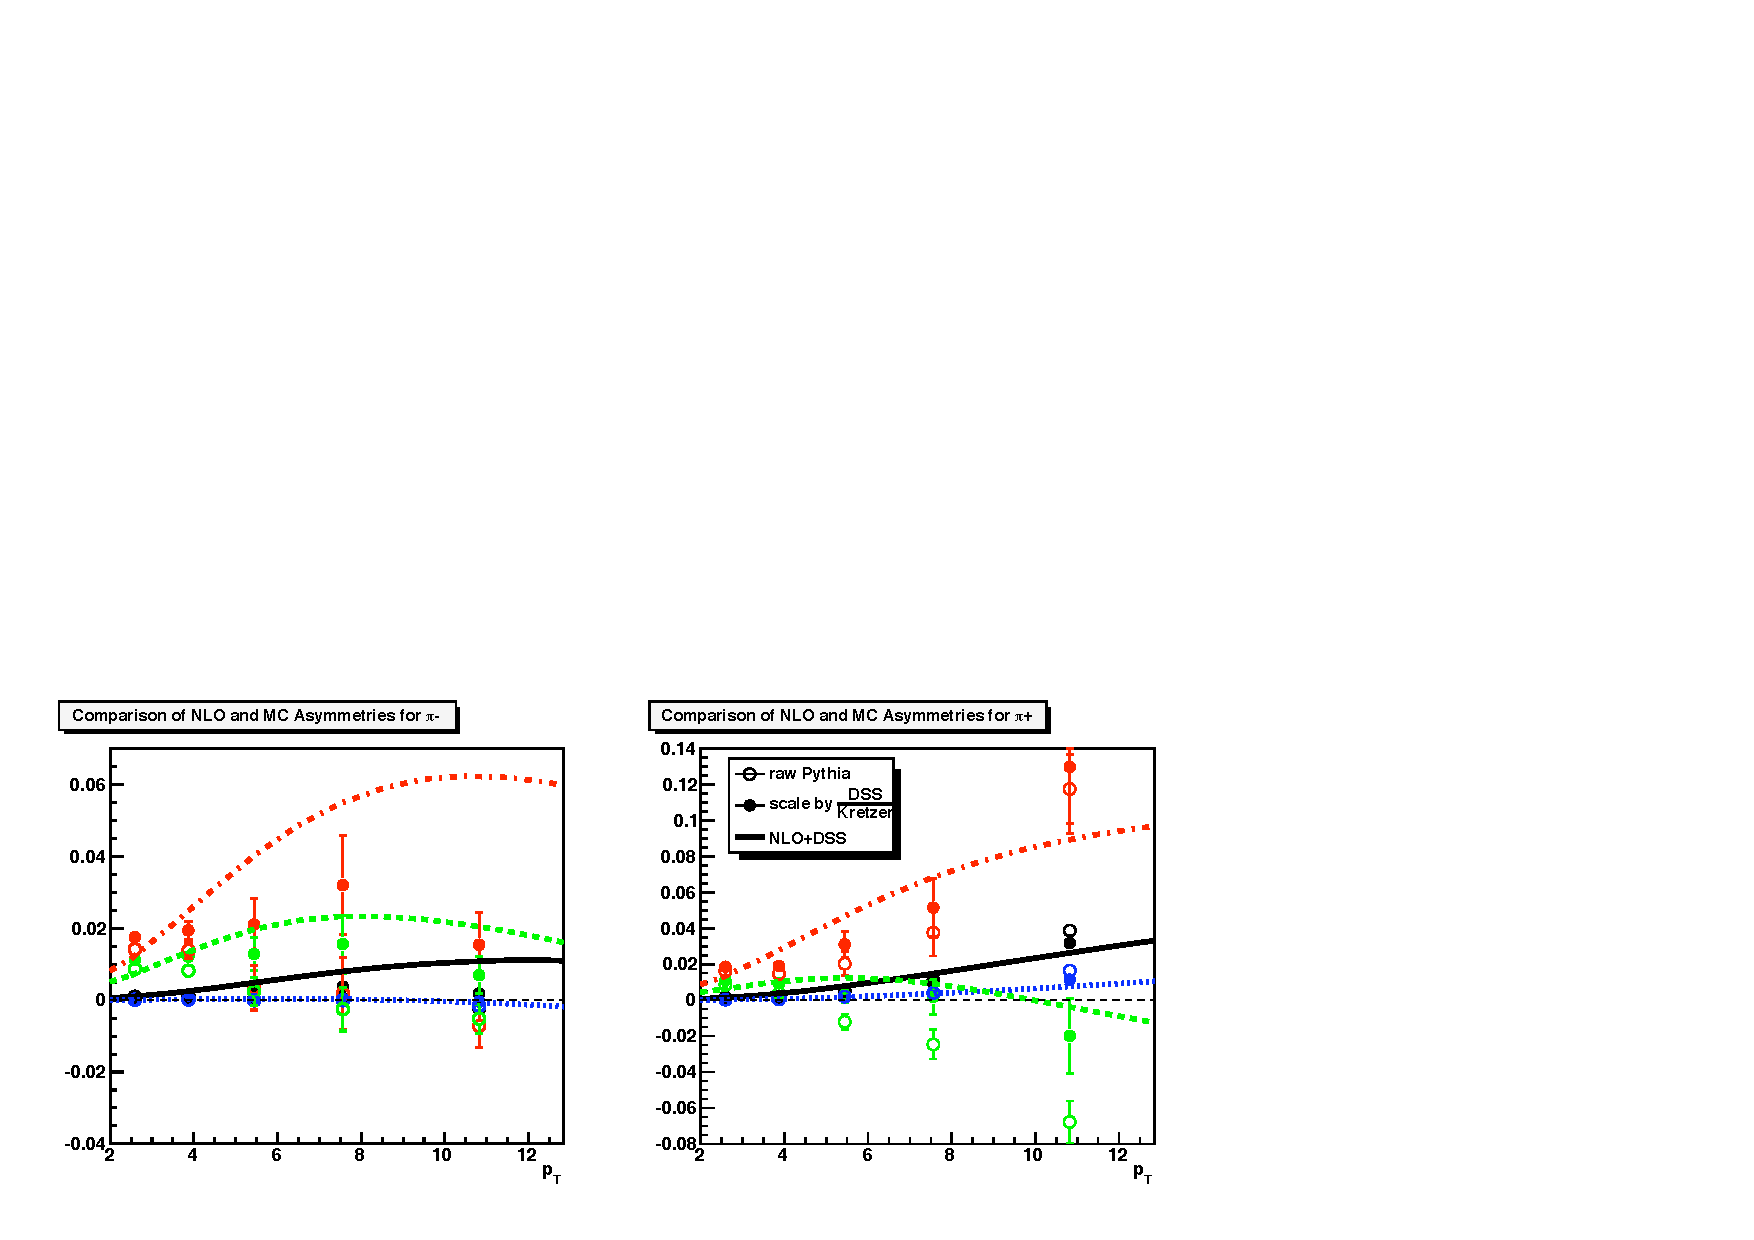
\includegraphics[width=\textwidth]{figures/compare-mcasym-nlo}
  \caption{Comparison of Monte Carlo asymmetries with NLO pQCD calculations
  incorporating DSS fragmentation functions. The open markers show results
  obtained using STAR's Pythia tune. The filled markers show the change in the
  asymmetries after reweighting the gg, qg, and qq distributions by the ratio
  of subprocess fractions calculated using DSS and Kretzer fragmentation
  functions.}
  \label{fig:compare-mcasym-nlo}
\end{figure}

Figure \ref{fig:mcasym-diff} examines the difference between asymmetries for a ``true'' sample using untriggered events and pions pulled straight from the Pythia record, and a ``trigger+reco'' sample where the events must satisfy the JP2 trigger simulator and the pion kinematics are obtained from TPC track reconstruction.  In some cases, the difference between the two samples is smaller than the uncertainty on the ``trigger+reco'' sample (see Figure \ref{fig:mcasym-sigma}).  We use the larger of the two to assign the systematic.

The size of the systematic obviously depends on the polarized gluon distributions that are included in the analysis.  Previous measurements have excluded the maximal polarization scenarios as well as scenarios with the functional form of the GRSV set and integral gluon polarizations larger than STD.  As a result, we use an envelope defined by the GRSV M105 and STD scenarios.  The results of this analysis are shown in Table \ref{tbl:trig-reco-bias}.

\begin{figure}
  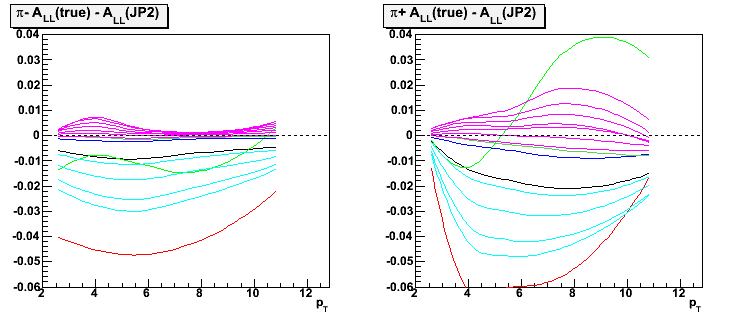
\includegraphics[width=\textwidth]{figures/mcasym_run5_diff_rescaled}
  \caption{Difference between true and reconstructed Monte Carlo
  asymmetries after fragmentation reweighting.}
  \label{fig:mcasym-diff}
\end{figure}

\begin{figure}
  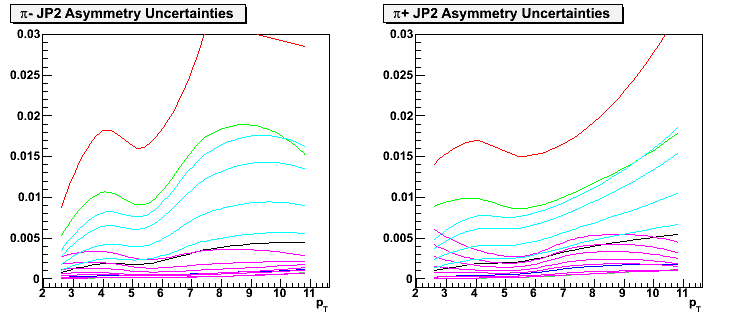
\includegraphics[width=\textwidth]{figures/mcasym_run5_sigma_rescaled}
  \caption{Uncertainty on reconstructed Monte Carlo asymmetries.  If the uncertainty is larger than the difference between true and reconstructed asymmetries we use this to assign the systematic instead.}
  \label{fig:mcasym-sigma}
\end{figure}

\begin{table}[ht]
    \begin{center}
        \begin{tabular}{c|c|c}
        \hline
        $p_{T}$ bin & $\pi^{-}$ uncertainty & $\pi^{+}$ uncertainty\\
        \hline
        \hline
        [2.00 - 3.18] & -0.0059 +0.0027 & -0.0061 +0.0061\\
        \hline
        [3.18 - 4.56] & -0.0083 +0.0072 & -0.0128 +0.0066\\
        \hline
        [4.56 - 6.32] & -0.0093 +0.0034 & -0.0176 +0.0101\\
        \hline
        [6.32 - 8.80] & -0.0072 +0.0036 & -0.0209 +0.0186\\
        \hline
        [8.80 - 12.84] & -0.0048 +0.0057 & -0.0152 +0.0062\\
    \hline
    \end{tabular}
    \end{center}
    \caption{Trigger and Reconstruction Bias Uncertainties}
    \label{tbl:trig-reco-bias}
\end{table}



%\chapter{Results and Discussion}

\section{$A_{LL}$ for Inclusive Charged Pion Production}

\begin{figure}[ht]
  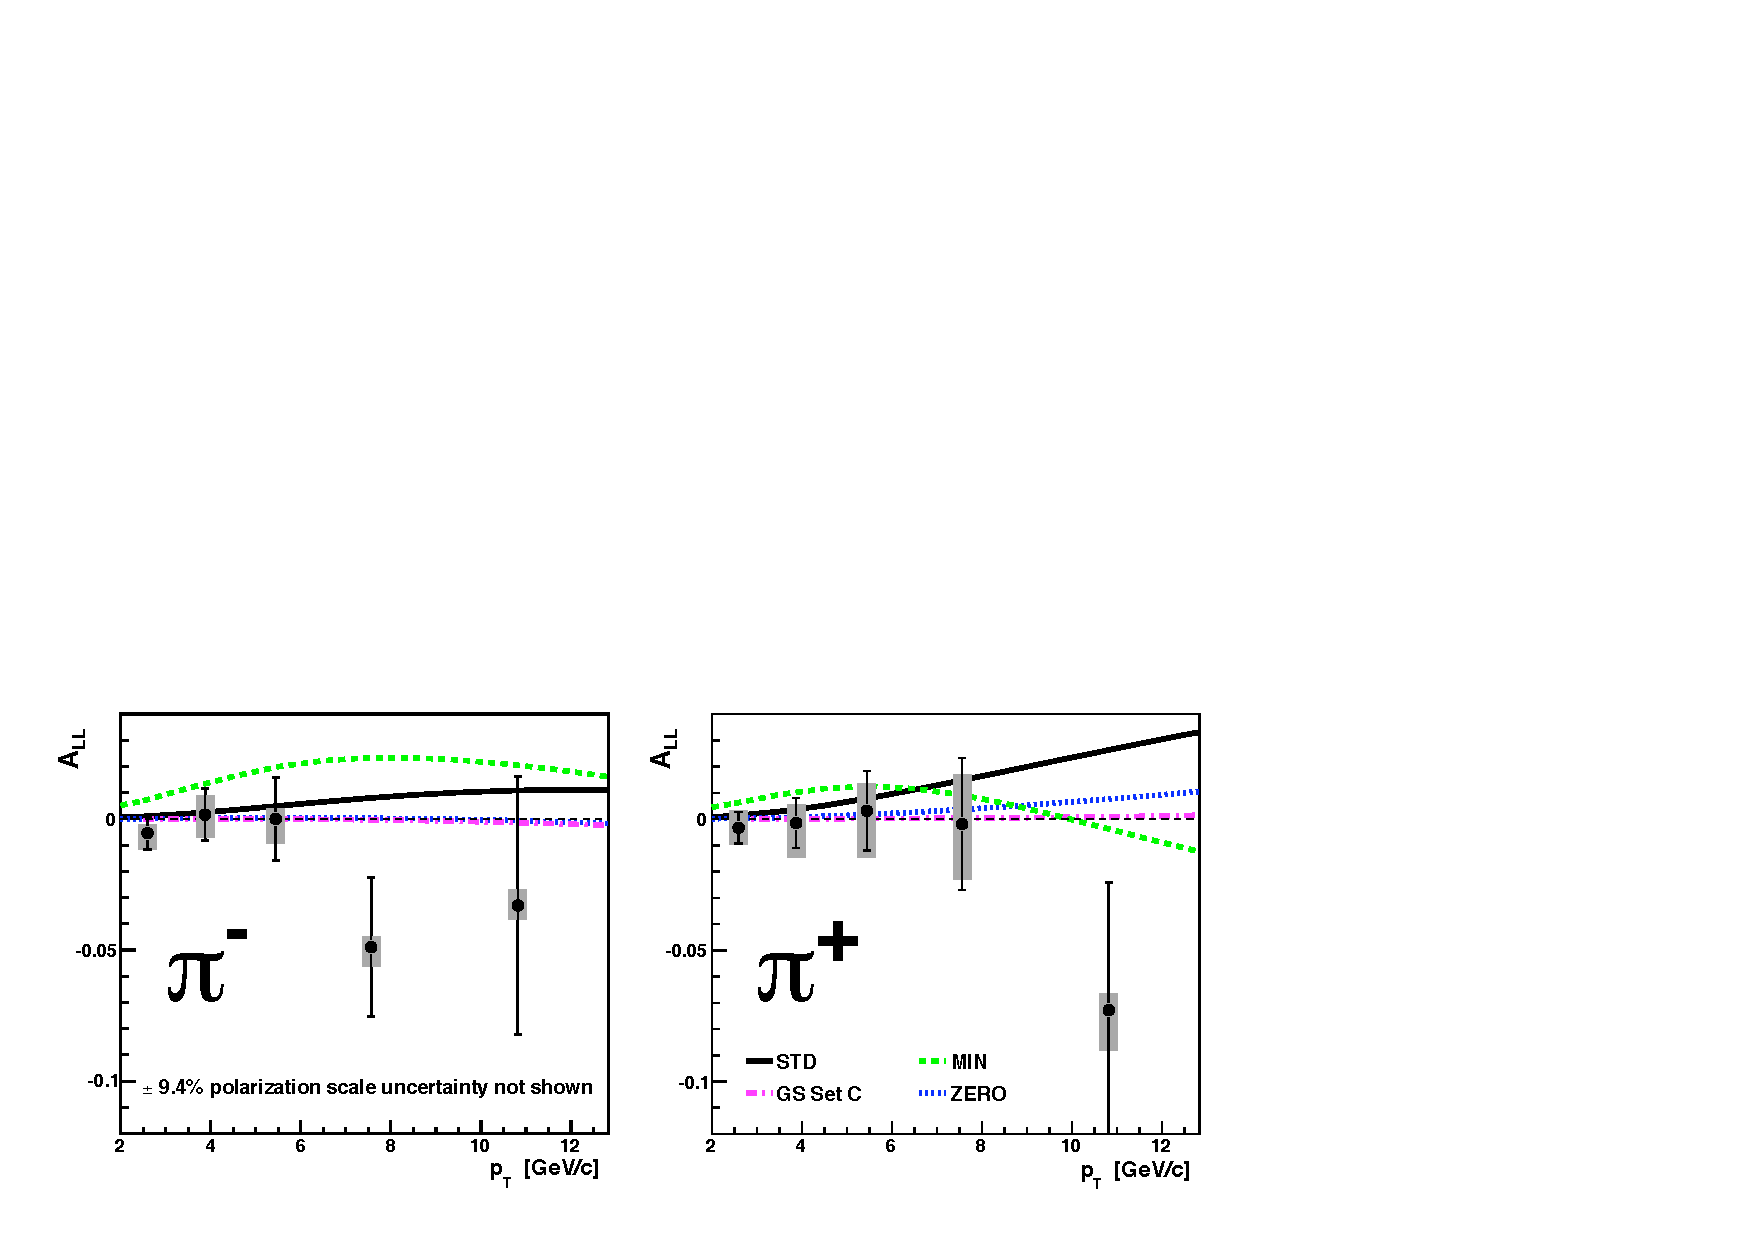
\includegraphics[width=1.0\textwidth]{figures/final-result-run5}
  \label{fig:final-result-run5}
\end{figure}

\section{$A_{LL}$ for Jet + Pion Correlations}

\begin{figure}[]
  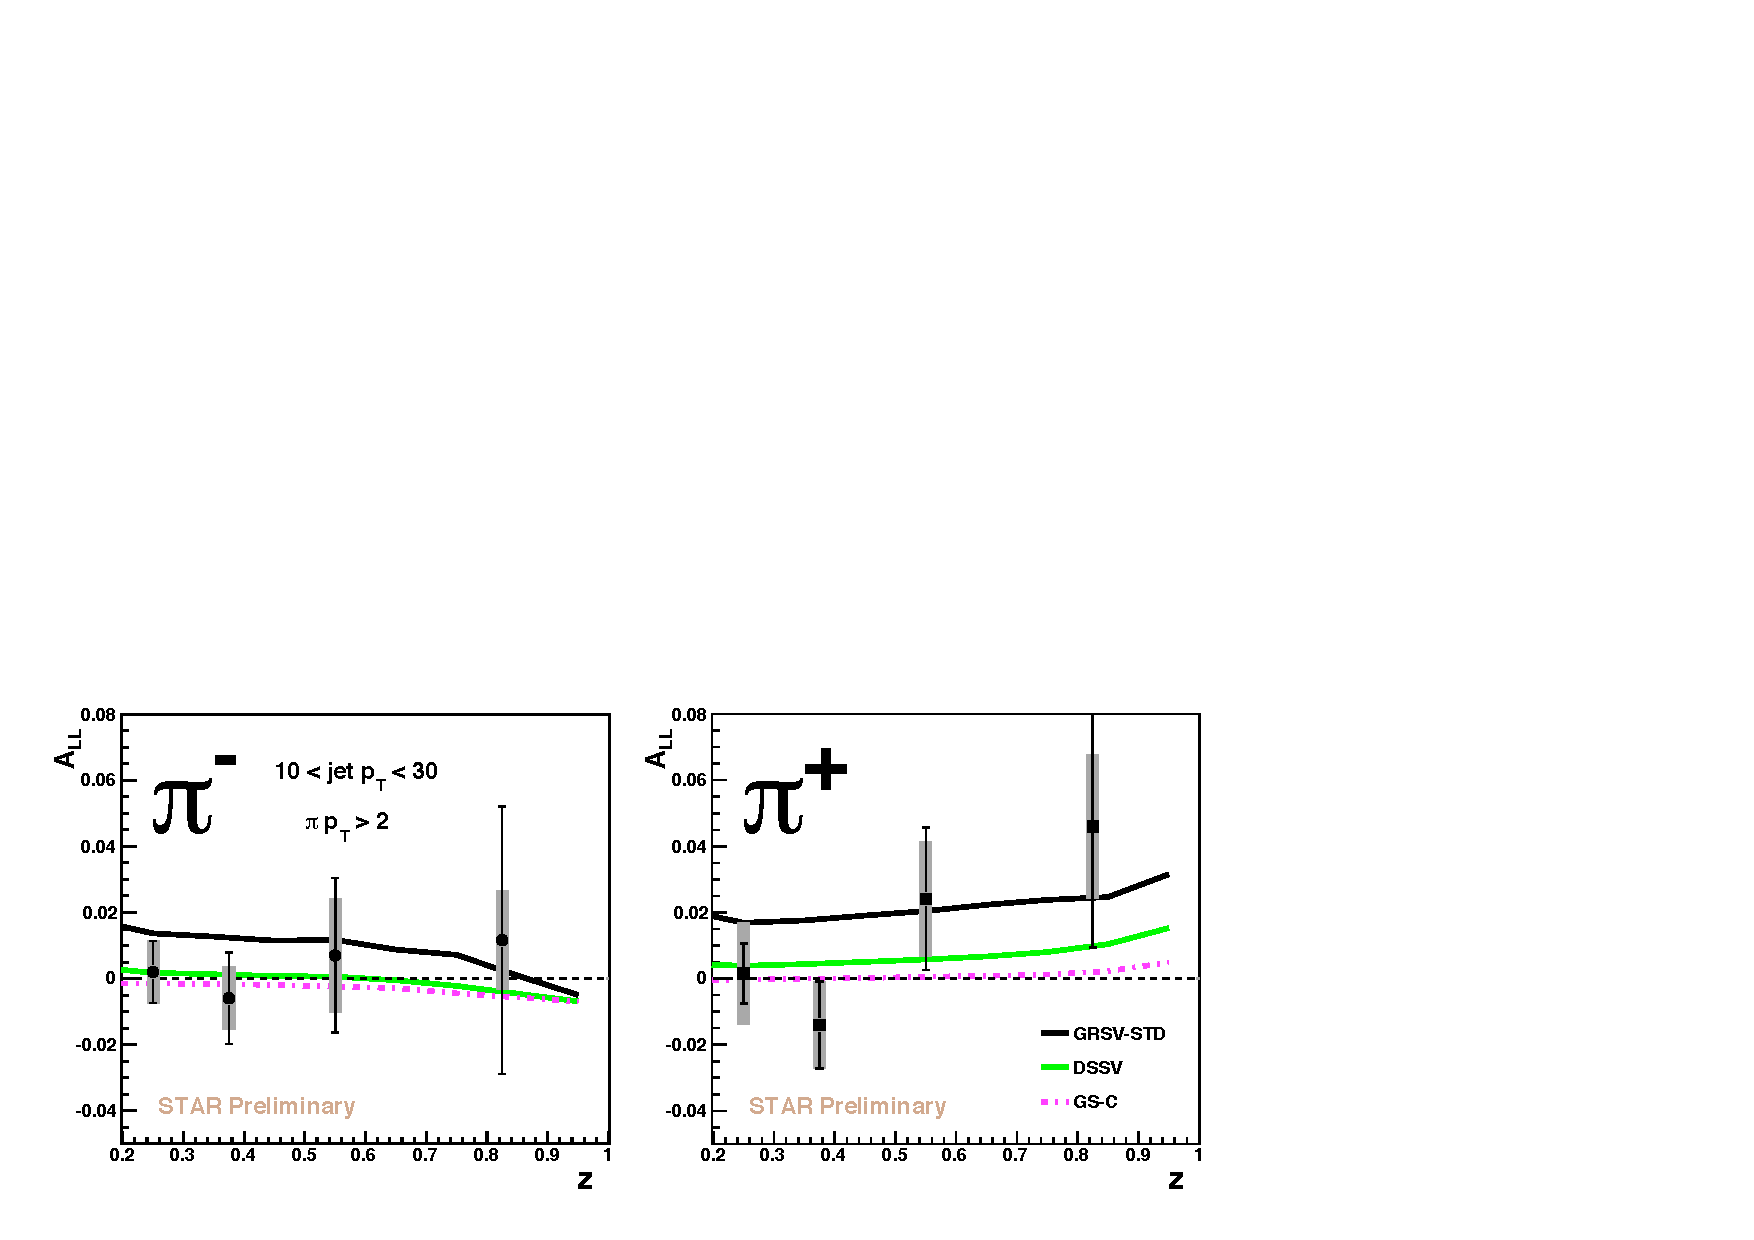
\includegraphics[width=1.0\textwidth]{figures/final-result-run6}
  \label{fig:final-result-run6}
\end{figure}

\section{Interpretation}

%\chapter{Conclusions}



\end{fmffile}
 \appendix
% \chapter{Tables}

\begin{table}
\caption{Armadillos}
\label{arm:table}
\begin{center}
\begin{tabular}{||l|l||}\hline
Armadillos & are \\\hline
our	   & friends \\\hline
\end{tabular}
\end{center}
\end{table}

\clearpage
\newpage

%% \chapter{Figures}

\vspace*{-3in}

\begin{figure}
\vspace{2.4in}
\caption{Armadillo slaying lawyer.}
\label{arm:fig1}
\end{figure}
\clearpage
\newpage

\begin{figure}
\vspace{2.4in}
\caption{Armadillo eradicating national debt.}
\label{arm:fig2}
\end{figure}
\clearpage
\newpage

\begin{singlespace}


%esta es la bibliografia standard de la IEEE
\bibliographystyle{IEEEtran}
\bibliography{IEEEabrv,bibliography/myIEEEbibliography}

%\bibliography{main}
%\bibliographystyle{plain}
\end{singlespace}
\end{document}

